\documentclass[oneside, final, 12pt]{article}

\pagestyle{plain}

\usepackage{a4wide}
\usepackage[utf8]{inputenc}
\usepackage[russian]{babel}
\usepackage{vmargin}
\setpapersize{A4}
\setmarginsrb{2cm}{1.5cm}{1cm}{1.5cm}{5pt}{5mm}{5pt}{13mm}
\usepackage{indentfirst}
\usepackage{graphicx}

\usepackage{amsmath}
\usepackage{amsfonts}
\usepackage{amsthm}
\usepackage{amssymb}

\def\Var{{\mathbb{V}\textrm{ar}}\,}
\def\E{{\mathbb{E} }\,}
\def\Cov{{\mathbb{C}\textrm{ov}}\,}
\def\P{{\mathbb{P} }\,}

\DeclareMathOperator*{\Argmax}{Arg\,max}

\newtheorem{theorem}{Теорема}
\newtheorem{definition}{Определение}
\newtheorem{statement}{Утверждение}
\newtheorem{consequence}{Следствие}
\newtheorem{remark}{Замечание}

\usepackage{subcaption}
\usepackage{caption}


\begin{document}

\thispagestyle{empty}

\begin{center}
\ \vspace{-3cm}

\includegraphics[width=0.5\textwidth]{msu.pdf}\\
{\scshape Московский государственный университет имени М.~В.~Ломоносова}\\
Факультет вычислительной математики и кибернетики\\
Кафедра системного анализа

\vfill

{\LARGE Отчёт по практикуму}

\vspace{1cm}

{\Huge\bfseries <<Стохастический анализ и моделирование>>}
\end{center}

\vspace{1cm}

\begin{flushright}
    \large
    \textit{Студент 415 группы}\\
    И.~А.~Кулешов
    \vspace{5mm}
    
    \textit{Руководитель практикума}\\
    к.ф.-м.н, доцент С.~Н.~Смирнов
\end{flushright}

\vfill

\begin{center}
Москва, 2019
\end{center}

\newpage
\tableofcontents

\newpage
\section{Задание 7}

\subsection{Постановка задачи}
    \begin{enumerate} 
        \item Методом случайного поиска найти минимальное значение функции $f$ на множестве 
        	$A = \{x_1, x_2: x_1^2+x_2^2\leqslant 1\}$, т.е. $y= \min\limits_{x\in A} f(x)$, где 
       	$$ f(x) = x_1^3\sin\left(\frac{1}{x_1}\right)+ 10 x_1 x_2^4 \cos\left(\frac{1}{x_2}\right)$$
       	при $x_1 \neq 0$ и $x_2 \neq 0$, функция доопределяется по непрерывности при $x_1=0$ или $x_2= 0$.
        \item Методом иммитации отжига найти минимальное значение функции Розенброка $g$ в пространстве
        		$\mathbb{R}^2$, где
        		$$ g(x) = (x_1 -1)^2+100(x_2-x_1^2)^2$$
        \item Оценить точность. Сравнить результаты со стандартными методами оптимизации.
    \end{enumerate}
\subsection{Решение задачи}
\subsubsection{Пункт 1}
	Для поиска минимального значения функции $f(x)$ будем $n$ раз разыгрывать случайные величины 
	$x_1$ и $x_2$ на множестве  $A = \{x_1, x_2: x_1^2+x_2^2\leqslant 1\}$, считать для каждой пары
	 значение функции $f(x_1, x_2)$ и затем из полученных $n$ значений выберем наименьшее.
	 \newline
	Рассмотрим следующую величину:
	$$
		\mathbb{P}((x_1,x_2) \in A) = \frac{1}{\pi} \iint\limits_{x_1^2+x_2^2\leqslant 1} dx_1dx_2 =  
														\frac{1}{\pi}\int\limits_0^1rdr\int\limits_0^{2\pi}d\varphi = 
														\int\limits_0^1dr^2\int\limits_0^{2\pi}\frac{1}{2\pi}d\varphi.
	$$
	В этом выражении был совершен переход к полярным координатам: 
	$$
		\begin{cases}
			x_1 = r \cos \varphi,\\
			x_2 = r \sin \varphi,
		\end{cases} 
		\quad  0 \geqslant r \leqslant 1, \quad  0 \geqslant \varphi \leqslant 2\pi.
	$$ 
	Сделаем замену вида: $u = r^2>0, u \in [0;1]$.
	Тогда окончательно получим:
	$$
		\mathbb{P}((x_1,x_2) \in A) = \int\limits_0^1du\int\limits_0^{2\pi}\frac{1}{2\pi}d\varphi.
	$$
	Отсюда видно, что совместное распределение $x_1$ и $x_2$ совпадает с совместным распределением
	случайных величин $u\sim U[0;1]$ и $\varphi\sim[0;\pi]$ (обоснование этого метода моделирования
	можно найти в задании 4). Выпишем выражения для $x_1$ и $x_2$:
	$$
		\begin{cases}
			x_1 = \sqrt{u}\cos \varphi, \\
			x_2 = \sqrt{u}\sin \varphi, 
		\end{cases}
		\quad u\sim U[0;1], 
		\quad \varphi \sim U[0;2\pi].
	$$	
	
	Теперь оценим погрешность данного метода. Пусть точка $(x^*, y^*)$ --- точка теоретического минимума,
	а точка $(x,y)$ --- это точка, полученная методом случайного поиска. Тогда:
	$$
		|f(x^*,y^*) - f(x,y)| \leqslant \max \limits_{(x,y)\in A}|\nabla f||(x^*,y^*) - (x,y)|.
	$$ 
	\newpage
	Оценим каждый из сомножителей:
	\begin{enumerate}
		\item Сначала $\max \limits_{(x,y)\in A}|\nabla f| =\max\limits_{(x,y)\in A} 
																				\sqrt{\left(\dfrac{\partial f}{\partial x_1}\right)^2 +
																							\left(\dfrac{\partial f}{\partial x_2}\right)^2}:$
				$$
					\begin{gathered}
						\left| \dfrac{\partial f}{\partial x_1}\right| =
					 		\left| 3x_1^2\sin\left(\frac{1}{x_1}\right)- x_1\cos\left(\frac{1}{x_1}\right)
					 					+ 10 x_2^4\cos\left(\frac{1}{x_2}\right) \right| \leqslant\\
					 		\leqslant \left| 3x_1^2\sin\left(\frac{1}{x_1}\right)\right| 
					 							+ \left|x_1\cos\left(\frac{1}{x_1}\right)\right|
					 							+ \left|10 x_2^4\cos\left(\frac{1}{x_2}\right) \right| \leqslant \sqrt{10} + 10, \\
					 	\left| \dfrac{\partial f}{\partial x_1}\right| = 
					 		\left| 10x_1\left(4x_2^3\cos\left(\frac{1}{x_2}\right)
					 				+x_2^2\sin\left(\frac{1}{x_2}\right) \right) \right| \leqslant 
					 				10 \left|4\cos\left(\frac{1}{x_2}\right)
					 						+\sin\left(\frac{1}{x_2}\right)\right| \leqslant 10\sqrt{17}.
					\end{gathered}
				$$
				Отсюда получаем оценку:
				$$
					|\nabla f| \leqslant 45.
				$$ 
		\item Теперь оценим $|(x^*,y^*) - (x,y)|$.
		
				Найдем, чему равна вероятность того, что точка $(x,y)$ попадет в $\varepsilon$-окрестность
				теоретической точки минимума $(x^*,y^*)$:
				$$	
					\mathbb{P} \Big( (x,y) \in B_{\varepsilon}(x^*,y^*)\Big) = \dfrac{\pi \varepsilon^2}{\pi} 
										= \varepsilon^2.
				$$
				Заметим, что исходная функция является четной по $y$, поэтому точек минимума будет
				две: если $(x^*, y^*)$ — точка минимума, то $(x^*,-y^*)$ — также точка минимума. Поэтому
				значение вероятности, равное $\varepsilon^2$, верно для случая, когда обе точки минимума
				лежат на границе множества $A$. Если же обе точки минимума лежат внутри множества,
				то существует две $\varepsilon$ --- окрестности, в которые может попасть очередная точка $(x, y)$, 
				значит, вероятность будет равна 2$\varepsilon^2$. Рассматривая худший случай, получаем, что 
				вероятность попасть методом случайного поиска в $\varepsilon$ --- окрестность точки минимума 
				равна $p=n\varepsilon^2$ . Тогда:
				$$
					|(x^*,y^*) - (x,y)| \leqslant \varepsilon = \sqrt{\dfrac{p}{n}}.
				$$
	\end{enumerate}
	Таким образом, мы получили оценку для метода случайного поиска:
	$$ |f(x^*,y^*) - f(x,y)| \leqslant 45 \sqrt{\dfrac{p}{n}}.$$
	
	\begin{table}[h!]
	\begin{center}
		\begin{tabular}{|c|c|c|c|}
			\hline $N$ & значение минимума & погрешность($p=0.99$) & время работы \\ \hline
				$10^5$ & -1,28 & 0,16 & 0,014 \\ \hline
				$10^6$ & -1,287 & 0,049 & 0,135 \\ \hline
				$10^7$ & -1,288 & 0,016 & 1,372 \\ \hline
				$10^8$ & -1,2885 & 0,0049 & 13,268 \\ \hline
		\end{tabular}
		\caption{Результаты поиска минимума функции методом случайного поиска.}
		\label{sample_table}
	\end{center}
	\end{table}
	
\newpage
\subsubsection{Пункт 2}   

	Теперь для минимизации функции $f(x)$, которую будем интерпретировать как энергию системы, 
	мы будем использовать метод имитации отжига. Опишем алгоритм его работы: 
	\begin{enumerate}
		\item Случайным образом выбираем начальную точку $x_0$, задаем начальную температуру $T_0$
			Текущее значение энергии $E$ устанавливаем равным $f(x_0)$.
		\item $k$-ая итерация основного цикла состоит из следующих шагов:
			\begin{enumerate}
				\item Сравнить энергию системы $E$ в состоянии $x$ с найденным на текщий 
						момент глобальным минимумом. Если $E=f(x)$ меньше, то изменить значение глобального 
						минимума.
				\item Сгенерерировать новую точку $x'$. В нашем случае мы будем генерировать ее по нормальному 
						закону с математическим ожиданием $(x_k,y_k)$ и дисперсией $\sigma^2T_k$, 
						где $T(k)= T(k-1) k_{temp}$ --- температура системы в момент $k$.
				\item Вычисляем значение $E'=f(x')$.
				\item Генерируем случайное число $\alpha$ из интервала $[0;1].$
				\item Если $\alpha < h(E'-E,T(k)) = \exp^{-(E'-E)\slash T(k)} $, то $x=x_i, E= E'$ и переходим к 
						следующей итерации. Иначе, повторить шаг (b), пока не будет найдена подходящая точка
						$x'$.
			\end{enumerate}
	\end{enumerate}

\newpage
\section{Задание 8}

\subsection{Постановка задачи}
   	Применить метод Монте-Карло к решению первой краевой задачи для двумерного уравнения Лапласа 
   	в единичном круге:
   	$$
   		\begin{cases}
   		 	\Delta u = 0, (x,y) \in D \\
   		 	u|_{\delta D} = f(x,y) \\ 
   		 	u \in C^2 (D), f \in C(\delta D) \\
   		 	D = \{x,y: x^2+y^2 \leqslant 1\}	   		
		\end{cases}
   	$$
   	Для функции $f(x,y)= x^2-y^2$ найти аналитическое решение и сравнить с полученным по методу
   	Монте-Карло.
\subsection{Решение задачи}
	Выберем на плоскости достаточно мелкую квадратную сетку с шагом $h$. Кооринаты узлов $x_i = ih,y_j = jh,$
	а значения функций в узлах $u(x_i,y_i)= u_{i,j}, f(x_i,y_i)= f_{i,j} .$
	\begin{definition}
		Узел сетки $(i, j)$ называют внутренним, если и он, и все четыре соседних с ним узла
		$(i -1,j), (i +1, j), (i, j-1), (i, j+1)$, принадлежат 
		$D+\delta D$. В противном случае узел $(i, j)$, принадлежащий $D+\delta D$, называют граничным.
		Остальные узлы сетки будем называть внешними.
	\end{definition}
	\noindent
	Составим разностную схему. 
	Первое уравнение $u_{xx}+u_{yy}=0$ перейдет в:
	\begin{equation}
		\dfrac{u_{i+1,j}-2u_{i,j}+u_{i-1,j}}{h^2} + \dfrac{u_{i,j+1}-2u_{i,j}+u_{i,j-1}}{h^2} = 0, \quad (i,j) \in D_h,
		\label{num_1}
	\end{equation}
	где $D_h$ --- множество внутренних точек для данной сетки. \newline
	Перепишем ($\ref{num_1}$) относительно $u_{i,j}$ и получим:
	\begin{equation}
		\begin{cases}
			u_{i,j} = \dfrac{1}{4} (u_{i,-1j}+u_{i+1,j}+u_{i,j-1} +u_{i,j+1}), & (i,j) \in D_h,\vspace{2mm} \\
			u_{i,j} = f_{i,j}, & (i,j) \in \delta D_h,
		\end{cases} \label{num_sys}
	\end{equation}
	где $\delta D_h$ --- множество граничных точек для данной сетки.
	
	Заметим, что решение данной системы существует и единственно, и при $h\rightarrow 0$ стремится 
	к решению задачи Дирихле. Опишем метод Монте-Карло для системы ($\ref{num_sys}$).
	
	Представим себе частицу $M$, которая совершается равномерное блуждание по узлам сетки. 
	Находясь в узле $(i, j)$ частица равновероятно может перейти  в один из 
	четырех соседних узлов $(i -1,j), (i +1, j), (i, j-1), (i, j+1)$, причем каждый переход не зависит
	от предыстории и положения точки. Блуждание заканчивается, как только попадает в граничную точку.
	
	Пусть $P(i,j,p,q)$ --- вероятность того, что траектория частицы, вышедшей из узла $(i,j)$, закончится в 
	граничной точке $(p,q)$. Так как рано или поздно частица неизбежно попадет на одну из точек границы,
	то: 
	$$
		\sum\limits_{(p,q)\in \delta D_h} P(i,j,p,q) = 1 
	$$
	$$  P(p',q',p,q) = 	\begin{cases}
										1,& (p'-p)^2+(q'-q)^2 = 0,\\
										0, & (p'-p)^2+(q'-q)^2 \neq 0,
								\end{cases} \quad
		\forall (p',q') \in \delta D_h 
	$$
	\newpage
	Составим сумму 
	$$
		\nu_{i,j} = \sum\limits_{(p,q)\in \delta D_h} P(i,j,p,q) f_{p,q}
	$$
	Если рассматривать $f(x,y)$ как случайную величину, принимающую значения $f_{p,q}$  на границе
	$\delta D_h$, то $\nu_{i,j}$ --- это математическое ожидание $f(x,y)$ в точке $(x_i,y_j)$. 
	Так как из внутреннего узла частица равновероятно попадет в один из 4 соседних узлов, 
	то по формуле полной вероятности:
	\begin{equation}
		\nu_{i,j} = \sum\limits_{(p,q)\in \delta D_h}  (P(i-1,j,p,q)+P(i+1,j,p,q)+P(i,j-1,p,q)+P(i,j+1,p,q))f_{p,q}.
		\label{t_8}
	\end{equation}
	Окончательно получим:
	\begin{equation}
		\begin{cases}
			\nu_{i,j} = \dfrac{1}{4} (\nu_{i,-1j}+\nu_{i+1,j}+\nu_{i,j-1} +\nu_{i,j+1}), 
								& \forall (i,j) \in D_h \vspace{1mm} \\
			\nu_{i,j} = f_{i,j}, & (i,j) \in \delta D_h
		\end{cases} \label{num_sys_2}
	\end{equation}
	Мы получили систему, аналогичную ($\ref{num_sys}$). 
	В силу закона больших чисел можно приближать $\nu_{i,j}$ по формуле:
	\begin{equation}
		\nu_{i,j} \approx \dfrac{1}{N} \sum\limits_{k=1} ^N f(p^{k},q^{k}), \quad (p^k,q^k)\in \delta D_h.
		\label{approx_8}
	\end{equation}
	
	Для ускорения работы данного метода несколько модифицируем ход его выполнения: 	
	будем рассматривать его в <<обратном времени>>. Частица, находясь во внутреннем узле, 
	в предыдущий момент времени могла равновероятно быть в одном из 4 соседних внутренних узлов
	(предыдущей точкой не может быть граничная точка). Это значит, что если мы выберем
	какую-то граничную точку $(k_0,l_0)$ и будем блуждать по аналогичному 
	алгоритму по узлам сетки до момента попадения в седующую граничную точку $(k_1,l_1)$, 
	то мы получим множество $\Omega$ тех точек, траектория <<прямого>> блуждания 
	которых могла бы закончится в $(k_0,l_0)$. В свою очередь, попав в $(k_1,l_1)$, мы повторим
	вышеизложенную процедуру <<обратного>> блуждания. По-сути, в каждой точке множества $\Omega$ мы 
	получаем слагаемое в выражение ($\ref{t_8}$), где $f(p,q)=f(k_0,l_0).$ Следовательно, если для каждой
	внутренней точки мы будем запоминать количество попаданий <<обратных блужданий>> и сумму их 
	значений на начальных граничных точках, то поделив данную сумму на количество попаданий получим 
	в точности ($\ref{approx_8}$). Для того, чтобы получить необходимую точность, будем блуждать в 
	<<обратном времени>> до тех пор, пока не побываем в каждой внутренней точке хотя бы $N$ раз.
	\newline
	
	Теперь рассмотрим аналитическое решение исходной задачи.
	\newline
	По теореме о существовании решения внутренней задачи Дирихле, решение существует.\newline
	Будем искать его с помощью метода неопределенных коэффициентов:
	$$
		u(x,y) = c_0+ a_1x +b_1y+a_2x^2+b_2y^2.
	$$
	Подставим это в исходную задачу:
	$$
		\begin{cases}
			\Delta u = u_{xx} + u_{yy} = 2a_2+2b_2 = 0, \\
			 u|_{x^2+y^2 = 1} =  c_0+ a_1x +b_1y+a_2x^2+b_2y^2 = x^2 - y^2, 
		\end{cases}
	$$
	Решая эту систему получим: $c_0=a_1=b_1=0, a_2=1, b_2 = -1 \Rightarrow u(x,y)= x^2-y^2$.
    \begin{figure}[h!]
		\centering
		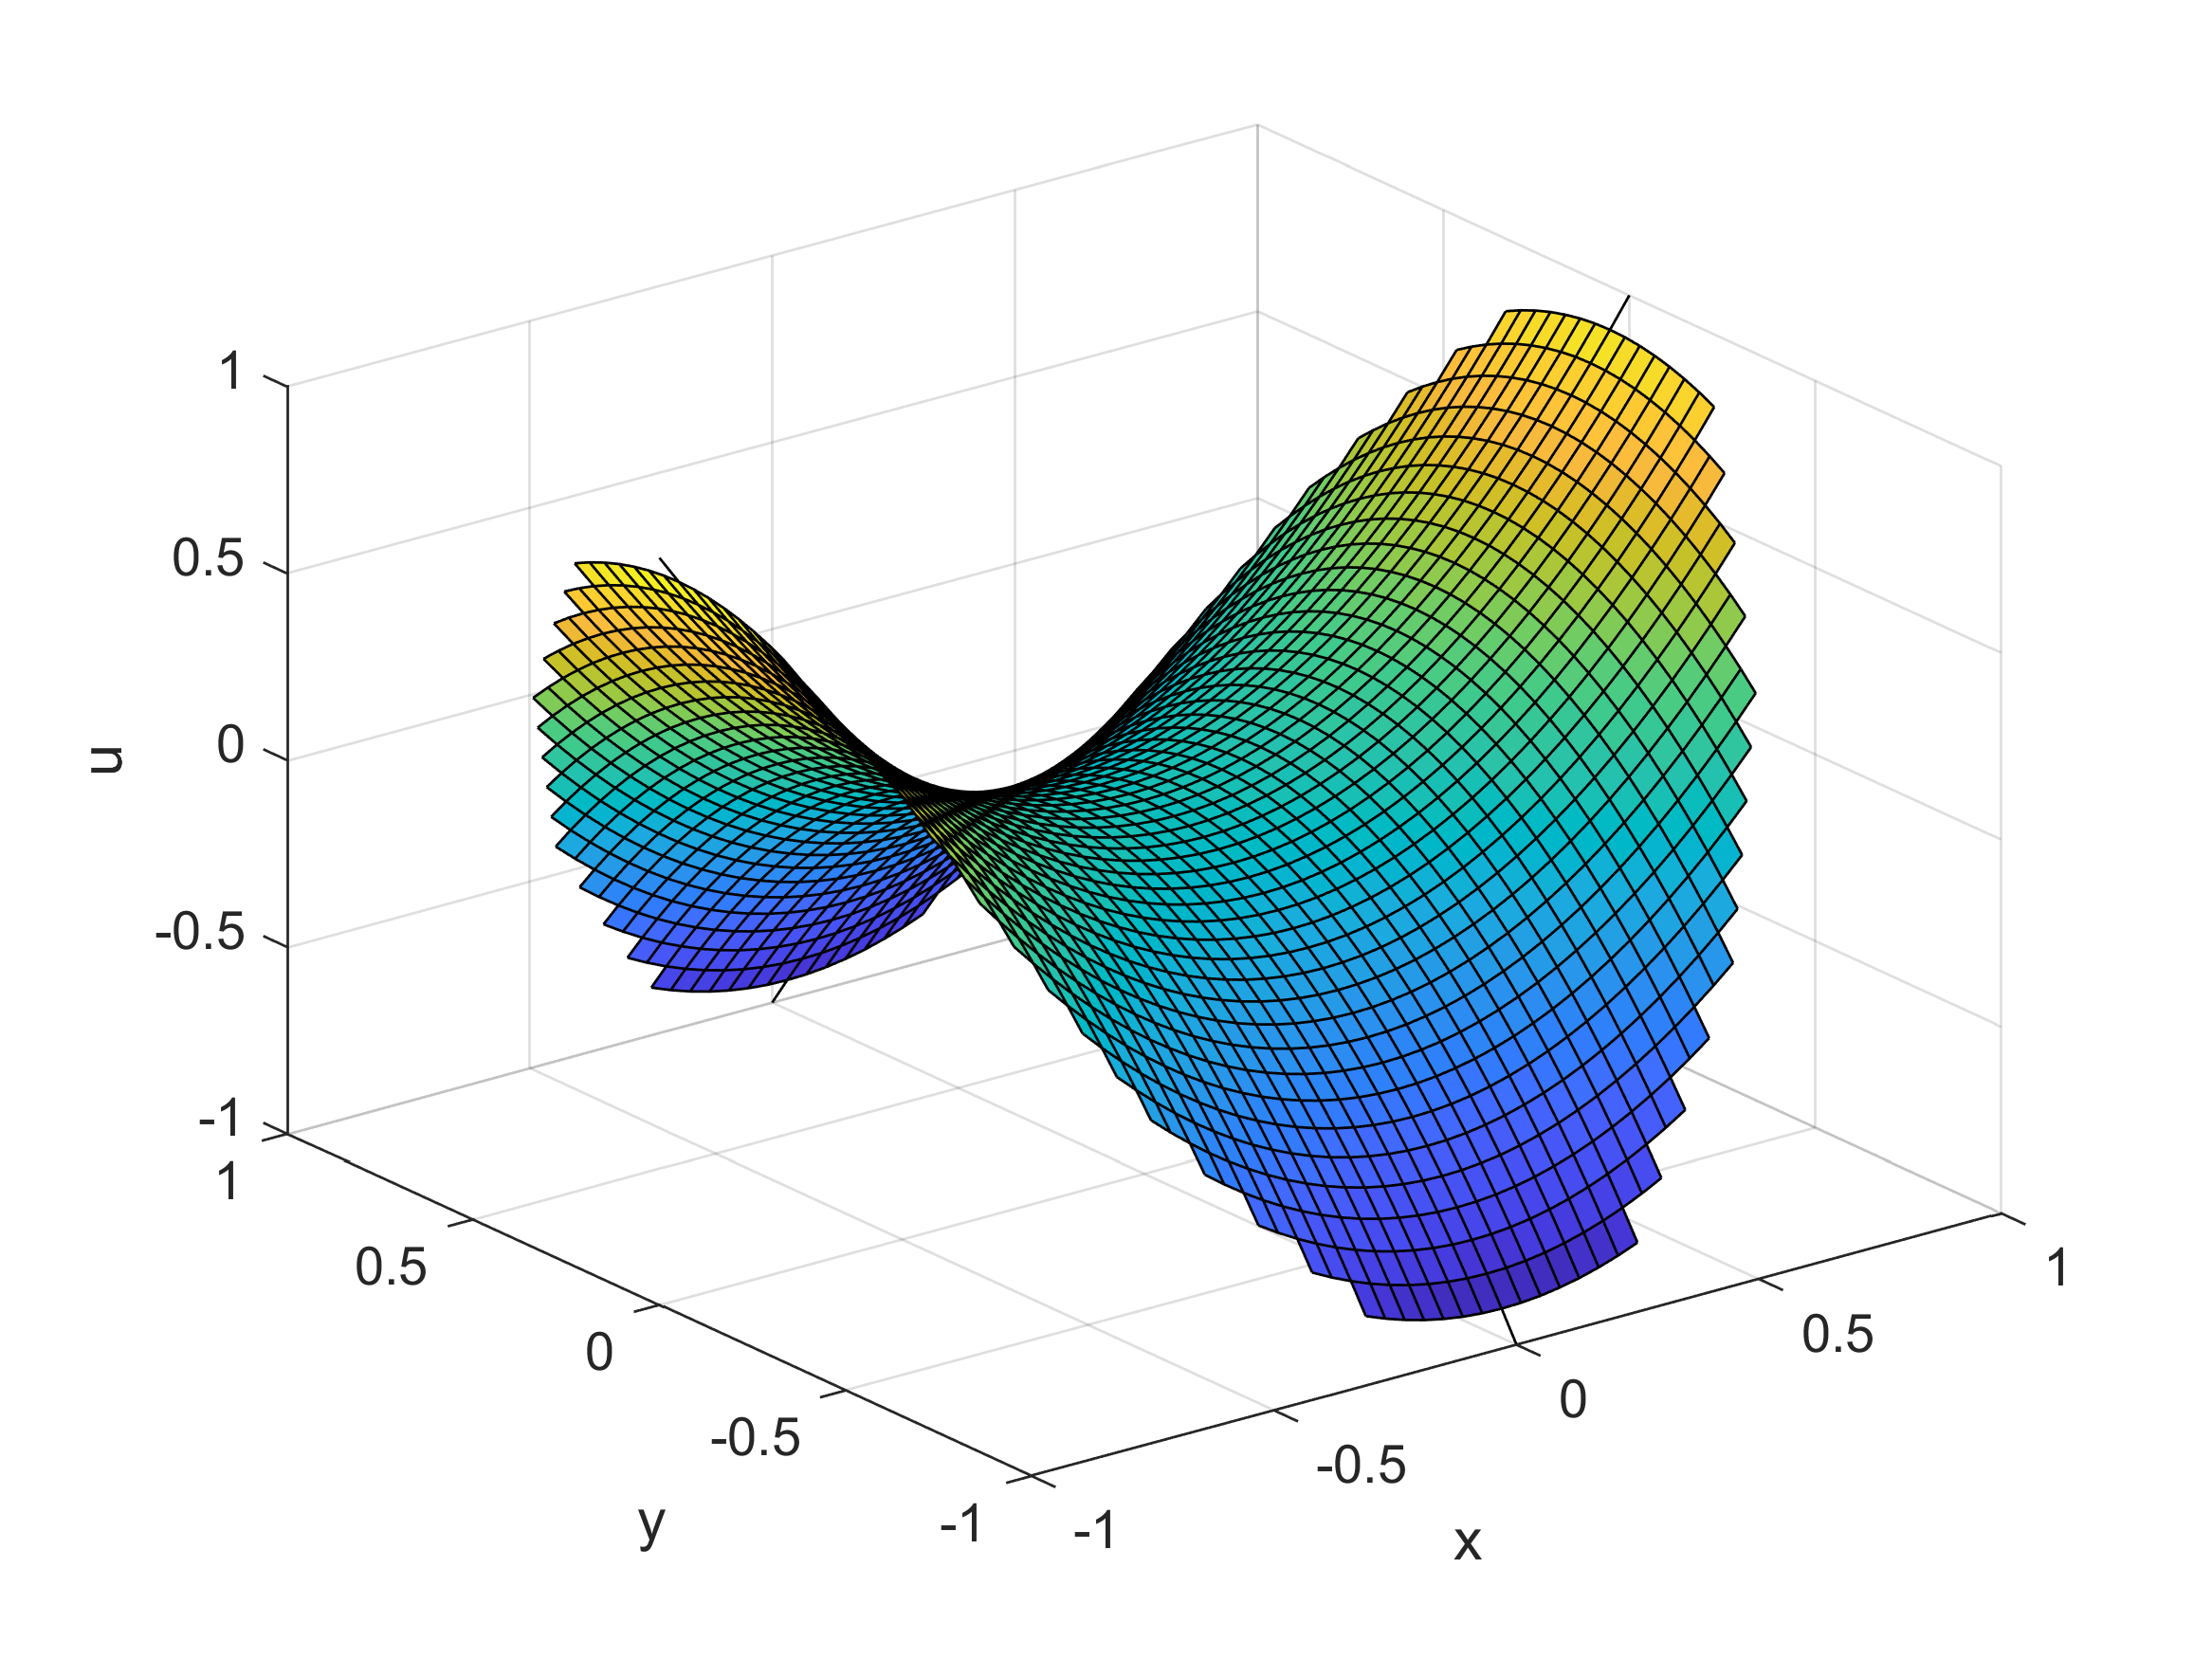
\includegraphics[width=0.6\textwidth]{../code/Task_8/pict/an_51_10000_ex.png}
		\caption{Аналитическое решении при $n = 51$ точках по каждой оси.}
    \end{figure}
   	\newpage
    \begin{figure}[h!]
		\centering
		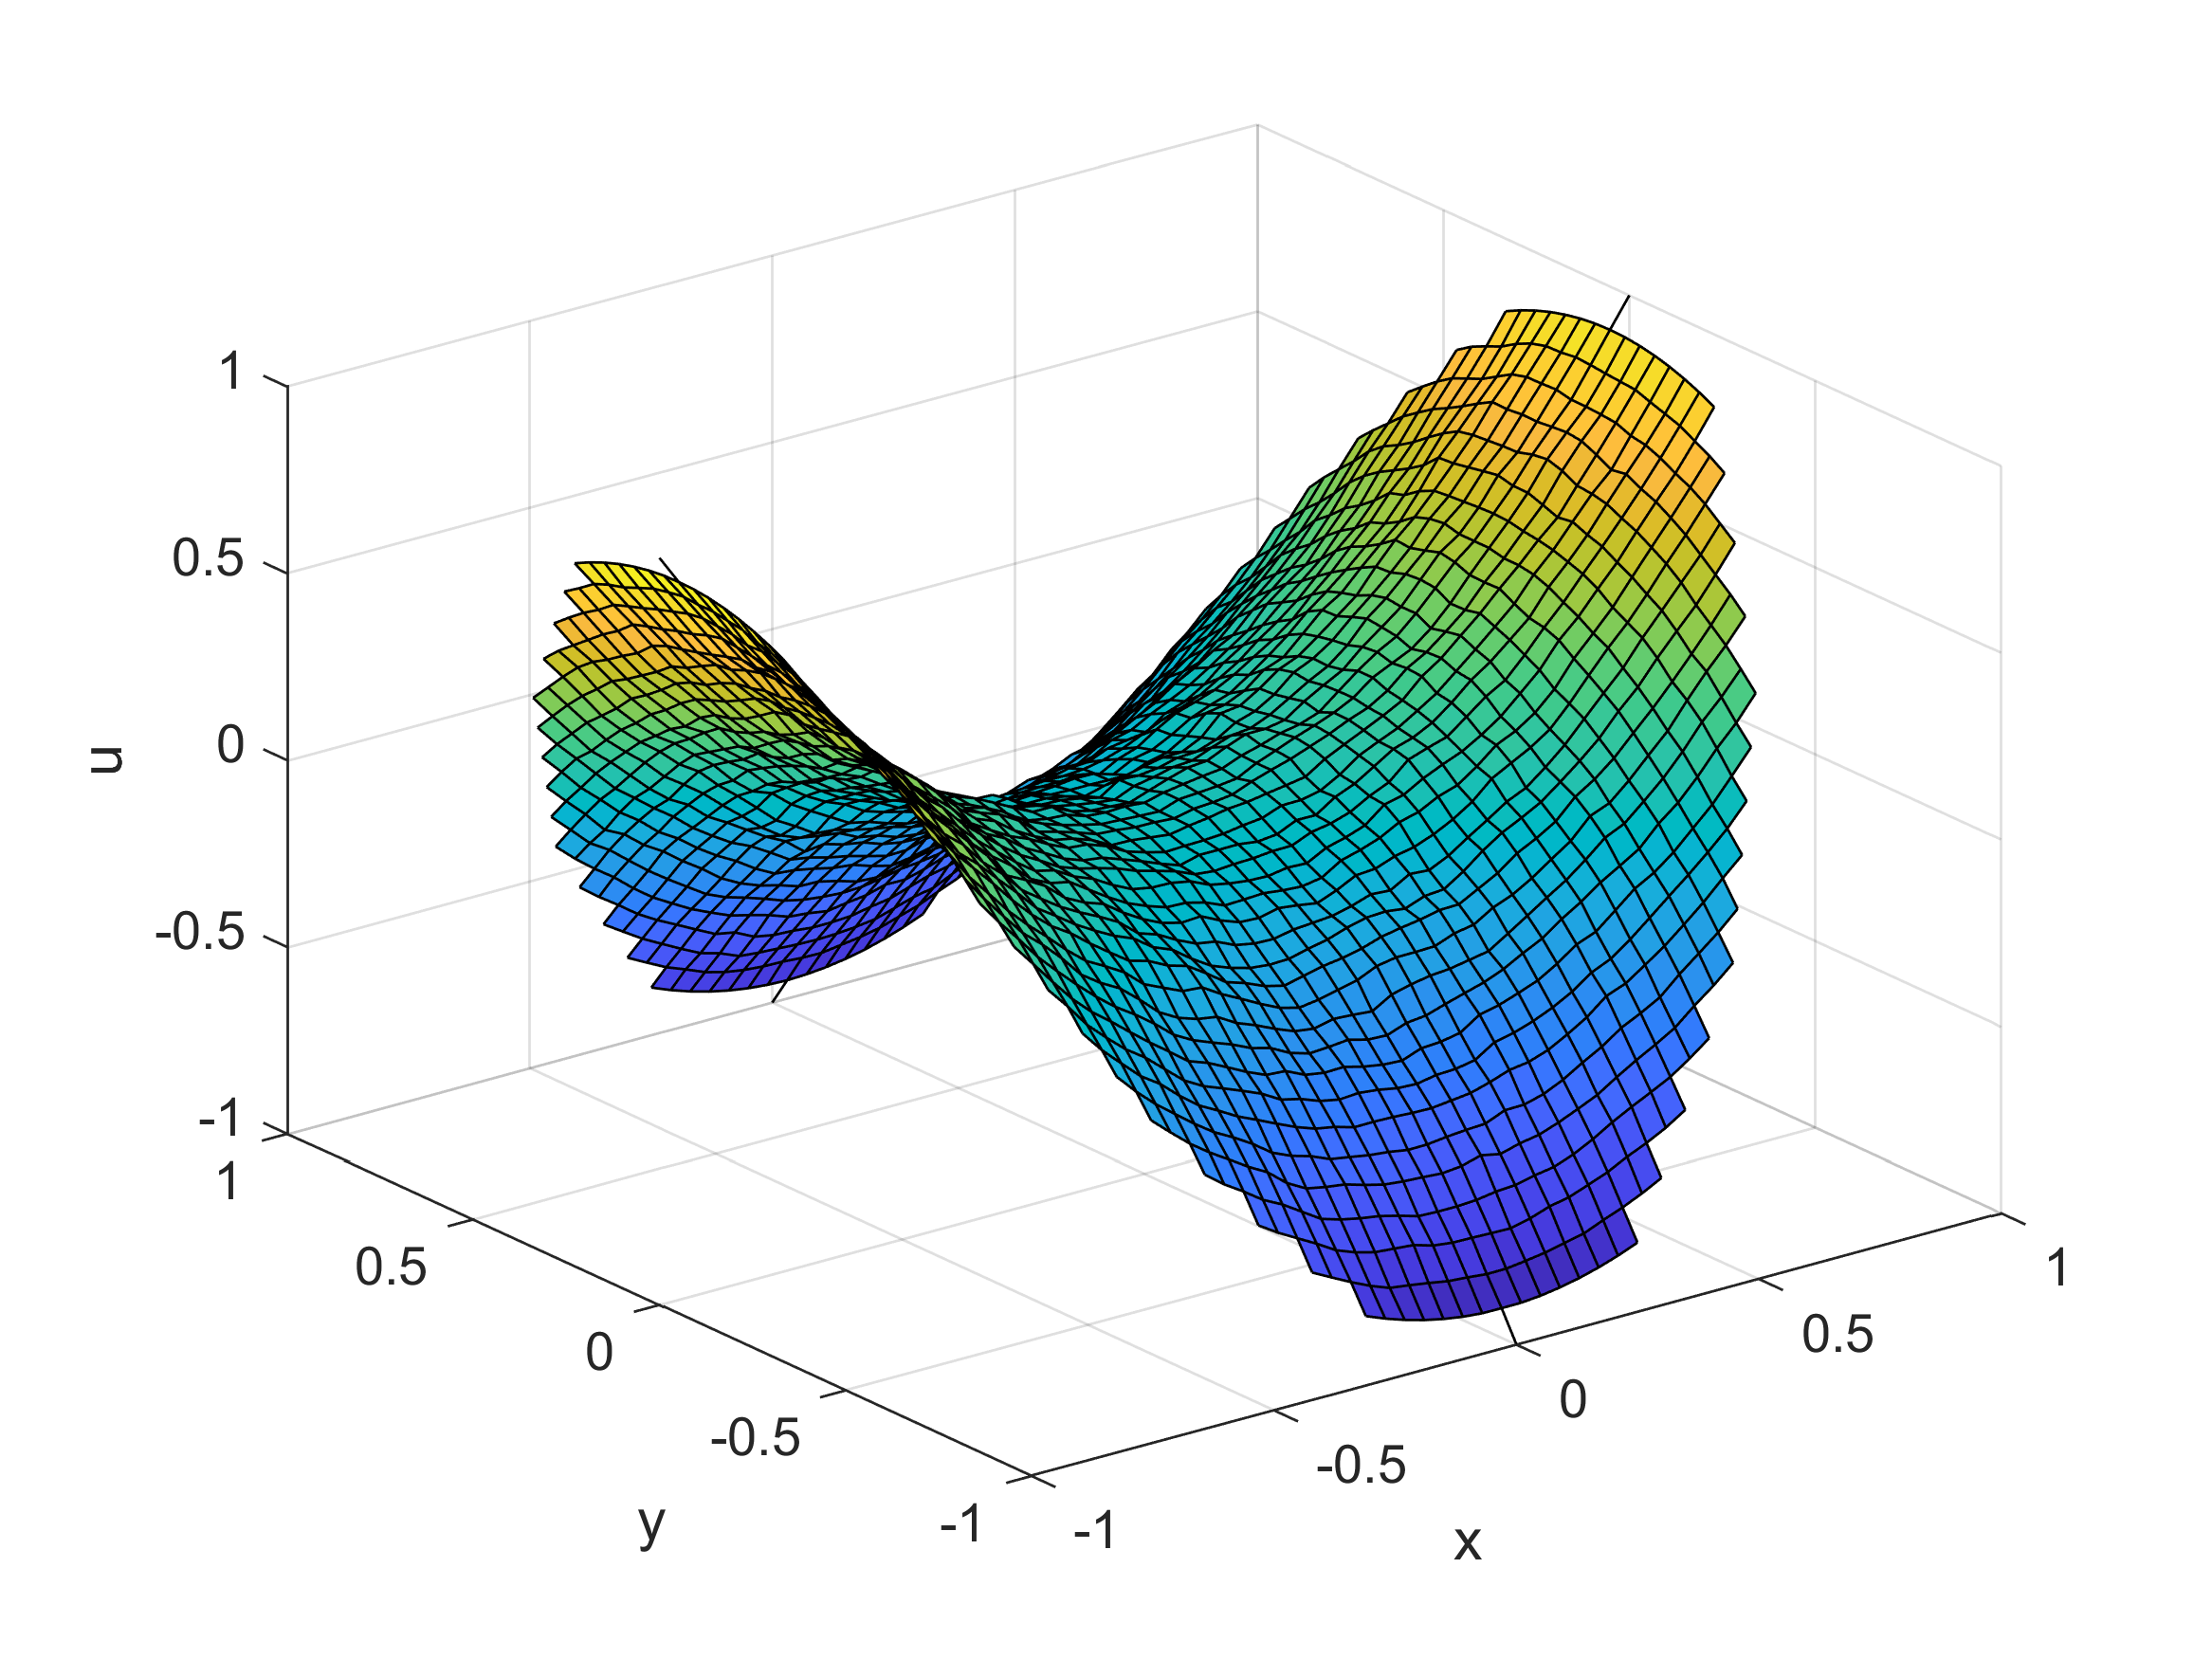
\includegraphics[width=0.6\textwidth]{../code/Task_8/pict/mc_51_10000_ex.png}
		\caption{Решение методом Монте-Карло с параметрами $n = 51, N =10000$. }
    \end{figure}
    \newpage
    \begin{figure}[h!]
		\centering
		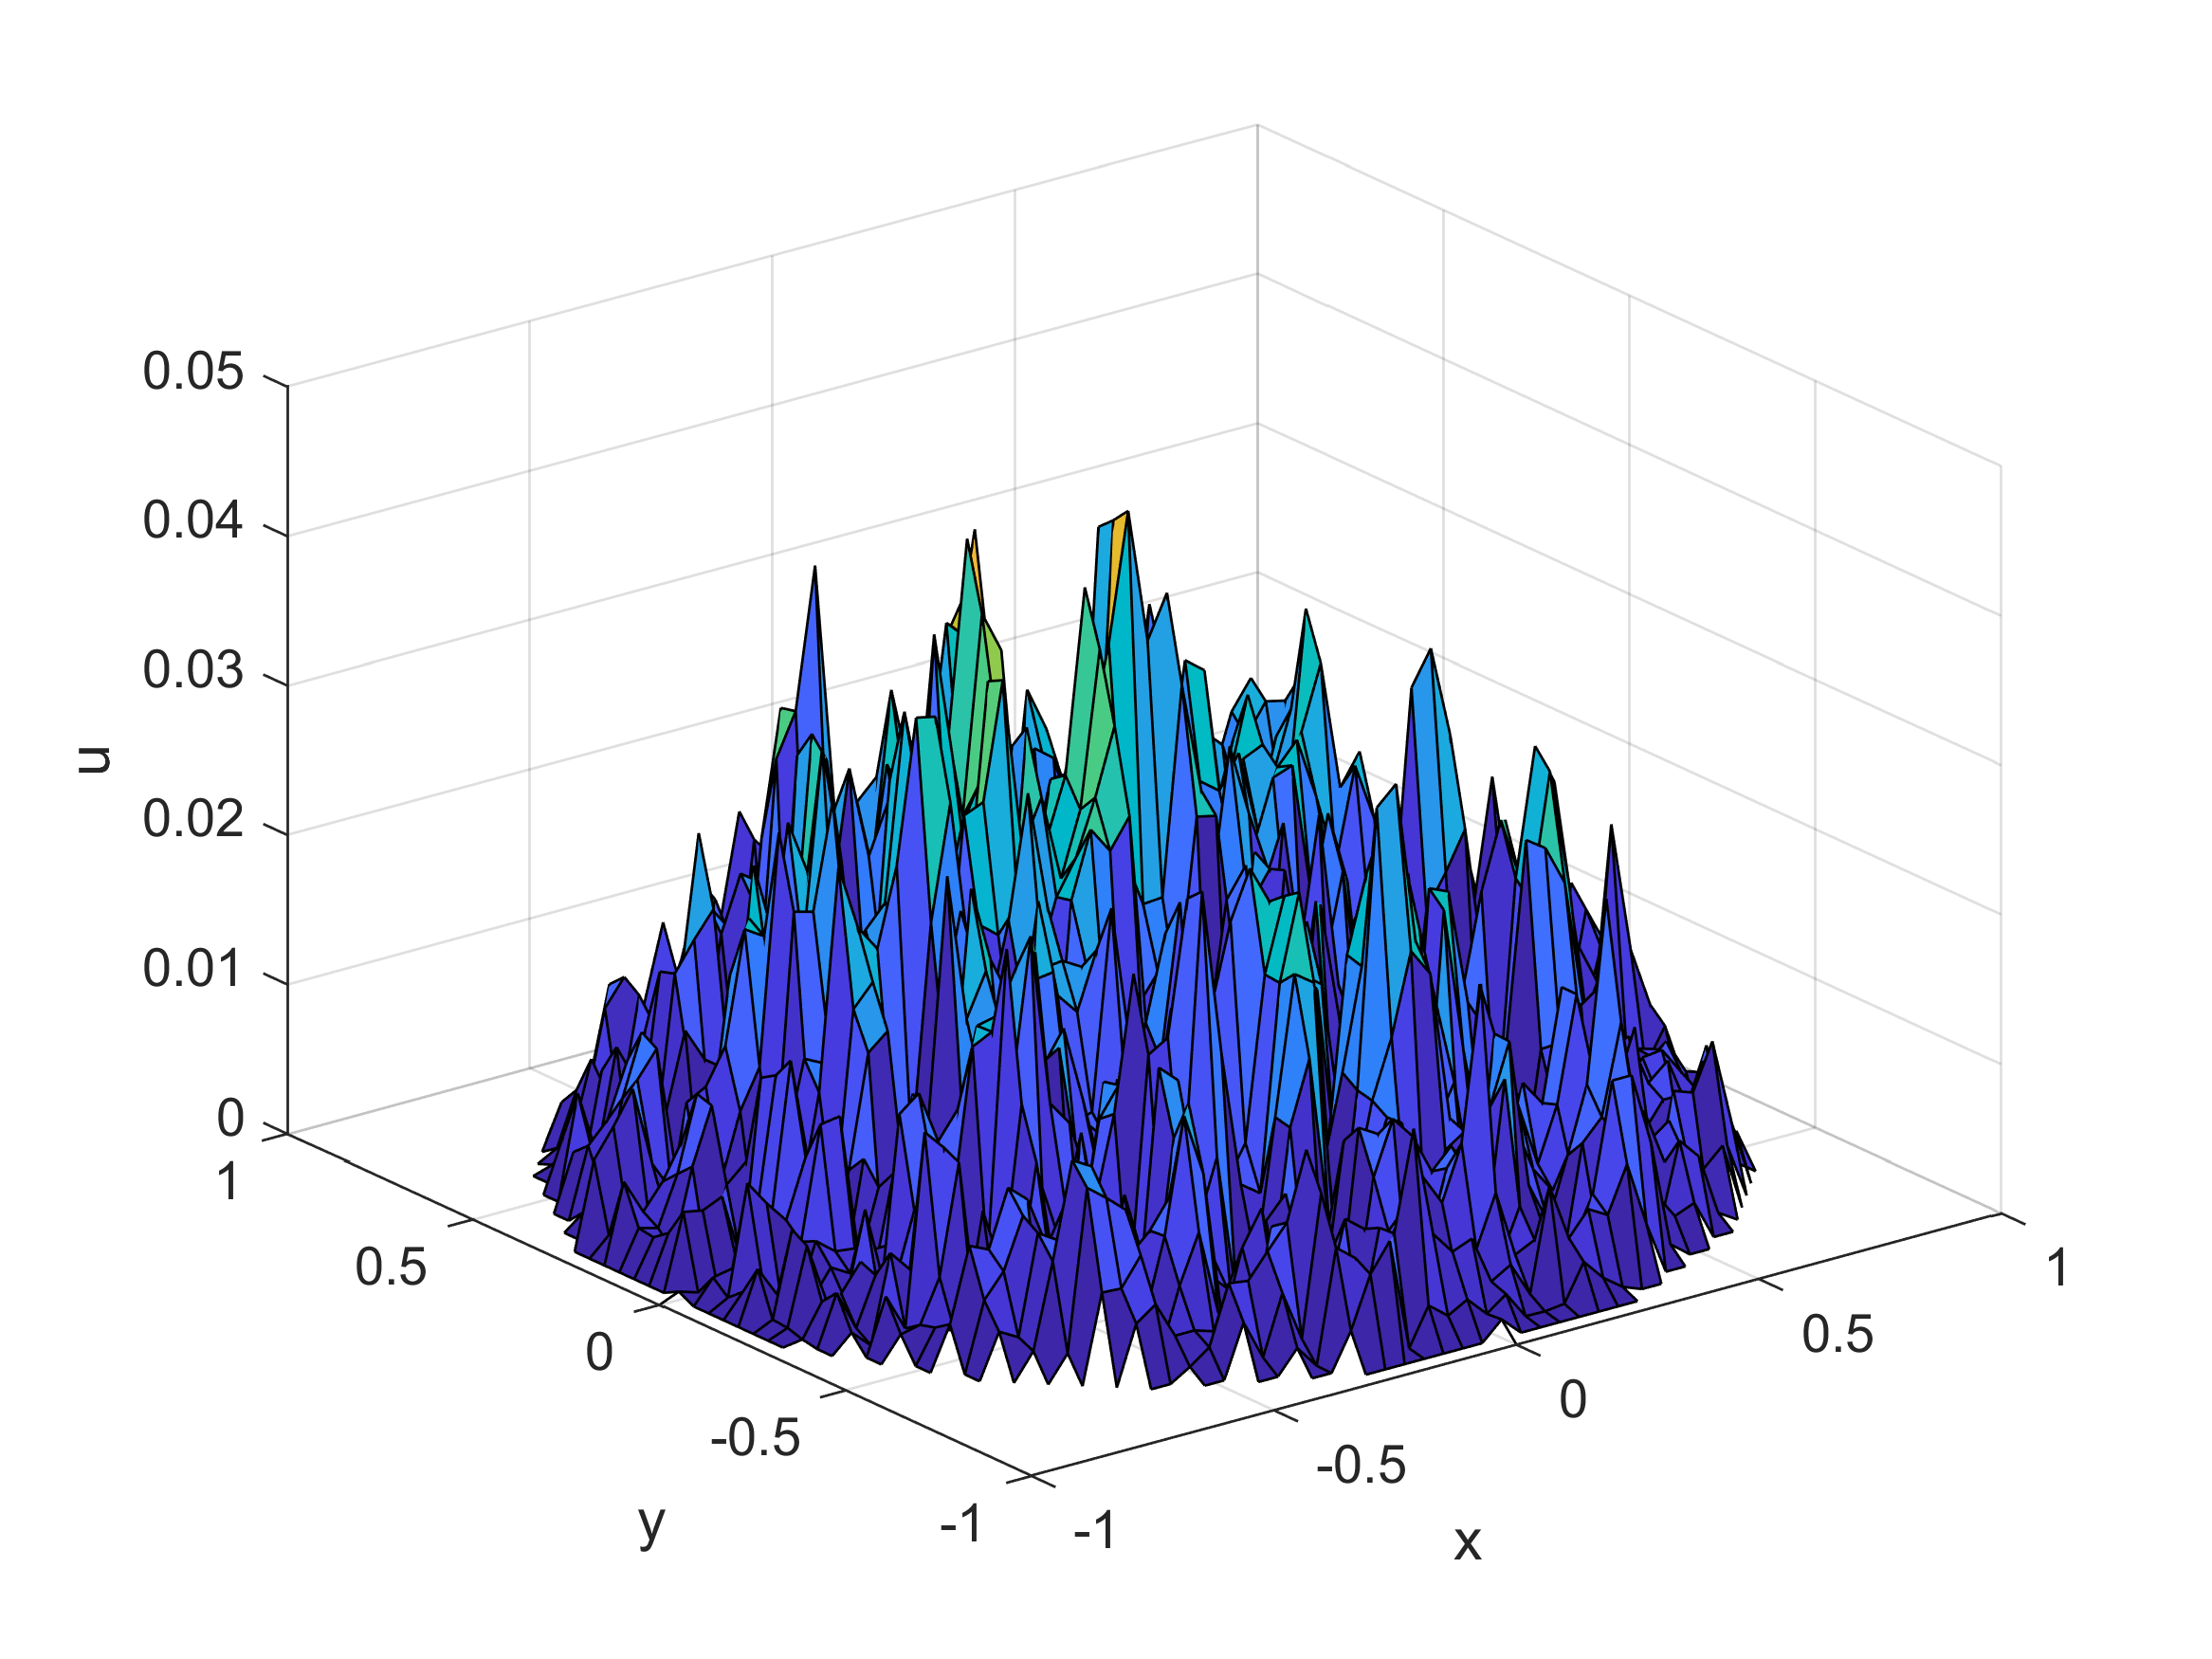
\includegraphics[width=0.6\textwidth]{../code/Task_8/pict/e_51_10000_ex.png}
		\caption{Ошибка методa Монте-Карло с параметрами $n = 51, N = 10000$. }
    \end{figure}
	
\newpage

\section{Задание 9}

\subsection{Постановка задачи}
	Рассмотреть два вида процессов:
	\begin{itemize}
		\item Винеровский процесс $W(t)$, $t \in [0;1]$, $W(0) = 0$.
		\item Процесс Орнштейна-Уленбека $X(t)$, $t \in [0;1]$, $X(0)=X_0$, то есть стационарный марковский 
				гауссовский процесс. Начальные значения $X_0$ генерируются случайным образом так, чтобы
				полученный процесс был стационарным.  
	\end{itemize}
	Для данных гаусовских процессов: 
    \begin{enumerate} 
        \item Найти ковариационную функцию и переходные вероятности.  
        \item Моделировать независимые траектории процесса с данными переходными вероятностями 
        		методом добавления разбиения отрезка. 
        \item Построить график траектории, не соединяя точки ломаной, с целью получения визуально
        		непрерывной линии.
    \end{enumerate}
\subsection{Решение задачи}
\subsubsection{Пункт 1}\
	Дадим несколько важных определений:
	\begin{definition}
		Пусть дано вероятностное пространство $(\Omega, \mathcal{F}, \mathbb{P})$.
		Параметризованное семейство $\{W_t |\, t \in T\}$ случайных величин вида: 
			$W_t(\cdot): \Omega \rightarrow \mathbb{R}, \,\, t\in T$, где $T\in[0,+\infty)$ и $T$ интерпретируется 
			как временной интервал, называется случайным процессом.
	\end{definition}
	\begin{definition}
		Случайный процесс $\{W_t |\, t \in T\}$ называется гаусовским, если
		$\forall n\geqslant 2, \forall t_1<t_2<\ldots<t_n \ \in T$ случайные величины
		$W_{t_1}, W_{t_2}, \ldots, W_{t_n}$ имеют многомерное нормальное распределение.
	\end{definition}
	\begin{definition}
		Случайный процесс $\{W_t |\, t \in T\}$ называется процессом с независимыми приращениями, если
		$\forall n\geqslant 2, \forall t_1<t_2<\ldots<t_n \in T$ случайные величины
		$W_{t_1}, W_{t_2}- W_{t_1}, \ldots, W_{t_n} -W_{t_{n-1}} $ независимы.
	\end{definition}
	Определим винеровский процесс на [0;1] как гауссовский с независимыми приращениями и $W(0)=0$ п.н.
	
	Т.к. процесс гауссовский, то из этого следует, что 
	$\forall t_1<t_2<\ldots<t_n \ \in T$ случайный вектор
	$(W_{t_1}, W_{t_2}- W_{t_1}, \ldots, W_{t_n} -W_{t_{n-1}})$ будет иметь многомерное 
	нормальное распределение. Это значит, что $W_1 - W_0 = W_1 - 0 = W_1 \sim N(0,1)$.
	\newpage
	Для данного процесса вычислим ковариационную функцию $R(t,s)= \Cov (W_t,W_s)$. 
	Для этого рассмторим случай, когда $0\leqslant s \leqslant t$:
	$$
		\begin{gathered}
			\begin{cases}
				W_s - W_0 = W_s \\
				W_s \text{ и } W_t - W_s \text{ независимы}
			\end{cases} \Rightarrow
			\Cov (W_s, W_t - W_s) = 0, \text{ но} \vspace{2mm} \\
			\Cov (W_s, W_t - W_s) = \Cov (W_s, W_t) - \Cov (W_s, W_s) = \Cov (W_s, W_t) -  \Var (W_s) = \\
				= \Cov (W_s, W_t)  -  s = 0  \Rightarrow \Cov (W_s, W_t) = s.
		\end{gathered}
	$$
	Аналогично рассматривается и второй случай. Получаем, что для винеровского процесса: 
	$$
		R(t,s)= \min (s,t).
	$$
	Будем строить траекторию винеровского процесса методом деления отрезка $[0;1]$ в отношении $\alpha$
	исходя из следующих соображений:
	\begin{itemize}
		\item $W_0 = 0, W_1 \sim N(0,1)$,
		\item Рассмотрим отрезок $[t_1,t_2]$ и его внутреннюю точку $t = t_1 + \alpha (t_2 - t_1)$  
					и условную плотность:
					$$
						p_{W_t}(x|W_{t_1} = x_1, W_{t_2} = x_2) = \dfrac{p_{W_{t_1},W_t,W_{t_2}}(x_1, x, x_2)}
																										{p_{W_{t_1},W_{t_2}}(x_1, x_2)}.
					$$
	\end{itemize}
	Обозначим $\bar{x} = (x_1,x, x_2)'$ и $\hat{x} = (x_1,x_2)'$, тогда плотности распределения этих векторов 
	будут равны:
	$$
		\begin{gathered}
			p_{W_{t_1},W_t,W_{t_2}}(\bar{x}) = \dfrac{1}{(2\pi)^{\frac{3}{2}} \sqrt{|R_1|}} 
																			e^{-\frac{1}{2}\bar{x}'R_1^{-1}\bar{x}},	 \\ 		
			p_{W_{t_1},W_{t_2}}(\hat{x}) = \dfrac{1}{2\pi \sqrt{|R_2|}} 
																			e^{-\frac{1}{2}\hat{x}'R_2^{-1}\hat{x}},				
		\end{gathered}
	$$
	где $R_1, R_2$ --- соответствующие матрицы ковариаций. Вспомним, что $R(t,s) = \min (s,t)$, поэтому:
	$$
		R_1 = \begin{pmatrix} t_1 & t_1 & t_1 \\ t_1 & t & t \\ t_1 & t & t_2 \end{pmatrix}, 
		R_2 = \begin{pmatrix} t_1 & t_1 \\ t_1 & t_2 \end{pmatrix}.
	$$
	Используя символьные вычисления $Matlab$ получим окончательно:
	$$
		p_{W_t}(x|W_{t_1} = x_1, W_{t_2} = x_2) = \dfrac{1}{\sqrt{2\pi\alpha(1-\alpha)(t_2 - t_1)}}
													\exp \left\{-\dfrac{(x - ((1-\alpha)x_1 +\alpha x_2) )^2}
																				{2\alpha(1-\alpha)(t_2 - t_1)}\right\}.
	$$
	Это значит, что $$W_t \sim N((1-\alpha)x_1 +\alpha x_2), \alpha(1-\alpha)(t_2 - t_1) ).$$
	\newline Пусть $n$ --- это количество шагов метода деления отрезка. Каждый шаг ---  это деление 
	всех отрезков, содержавшихся в $[0;1]$ на шаге $n-1$, в соотношении $\alpha$. Количество точек 
	при моделировании равно $2^{n}+1$ на отрезке $[0;1]$.
	
	\begin{figure}[h!]
		\centering
		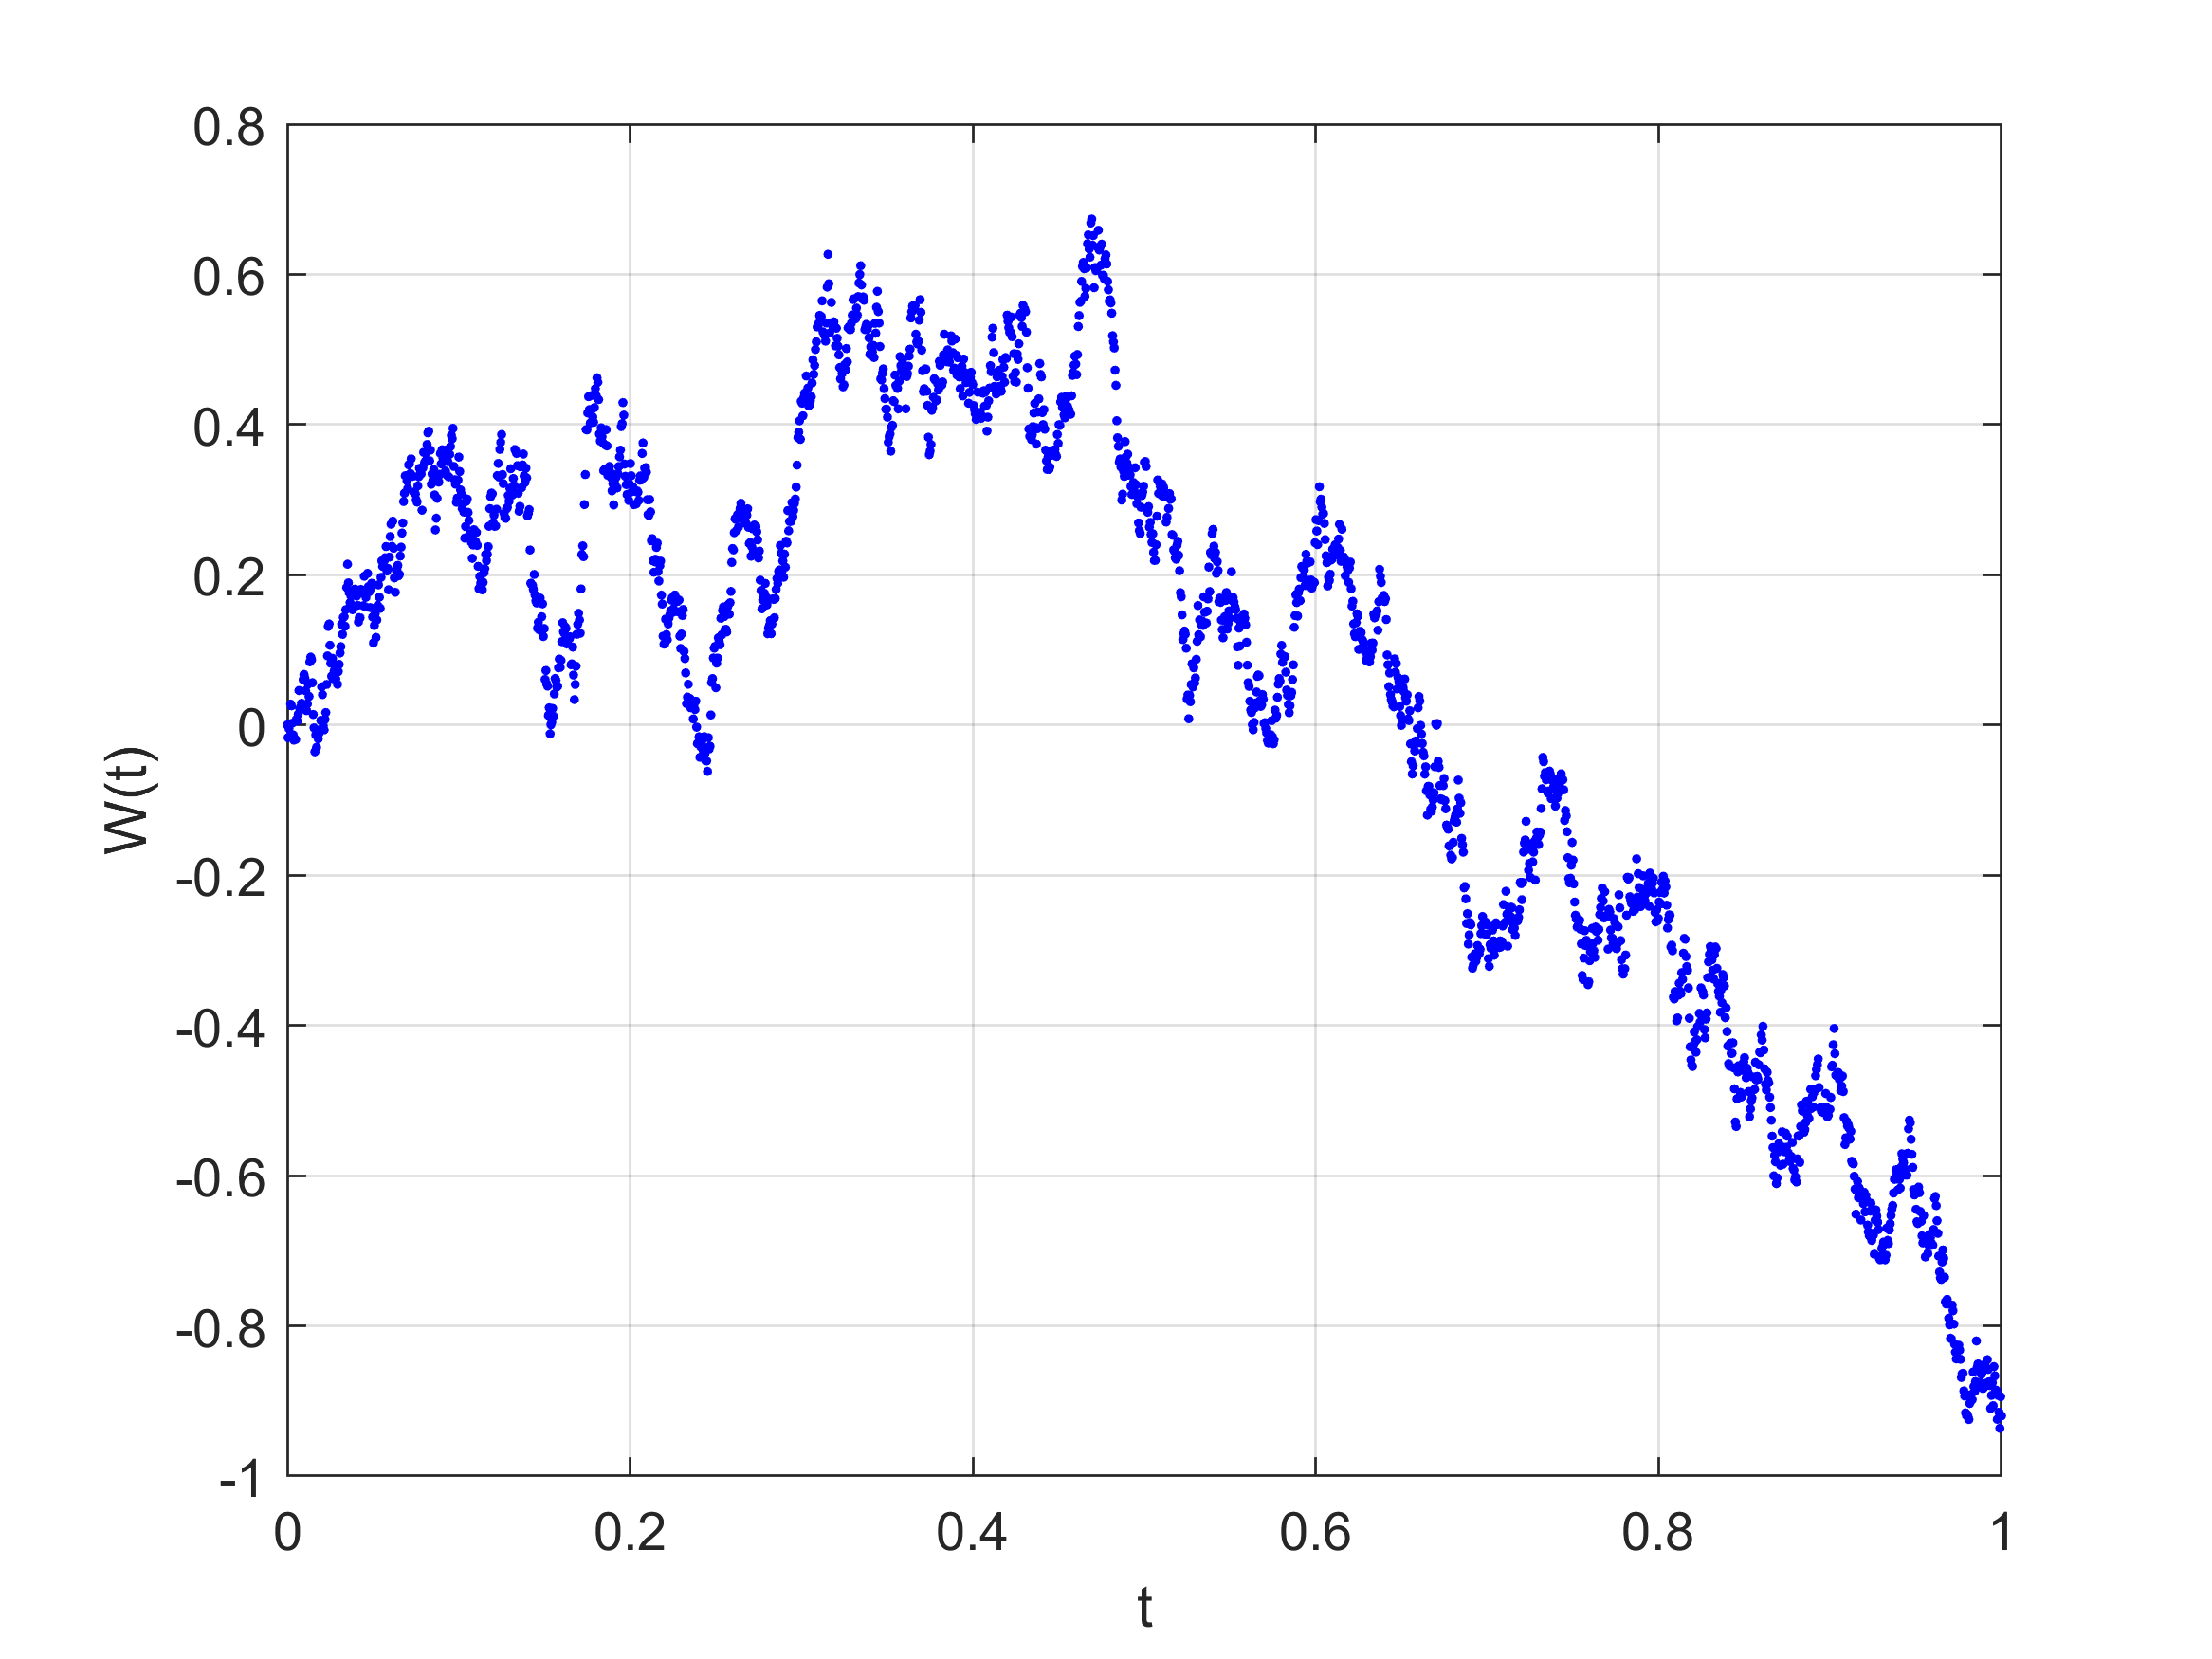
\includegraphics[width=0.6\textwidth]{../code/Task_9/pict/w_11_5_ex.png}
		\caption{Винеровский процесс с параметрами $n = 11, \alpha = 0.5$. }
    \end{figure}
    \begin{figure}[h!]
		\centering
		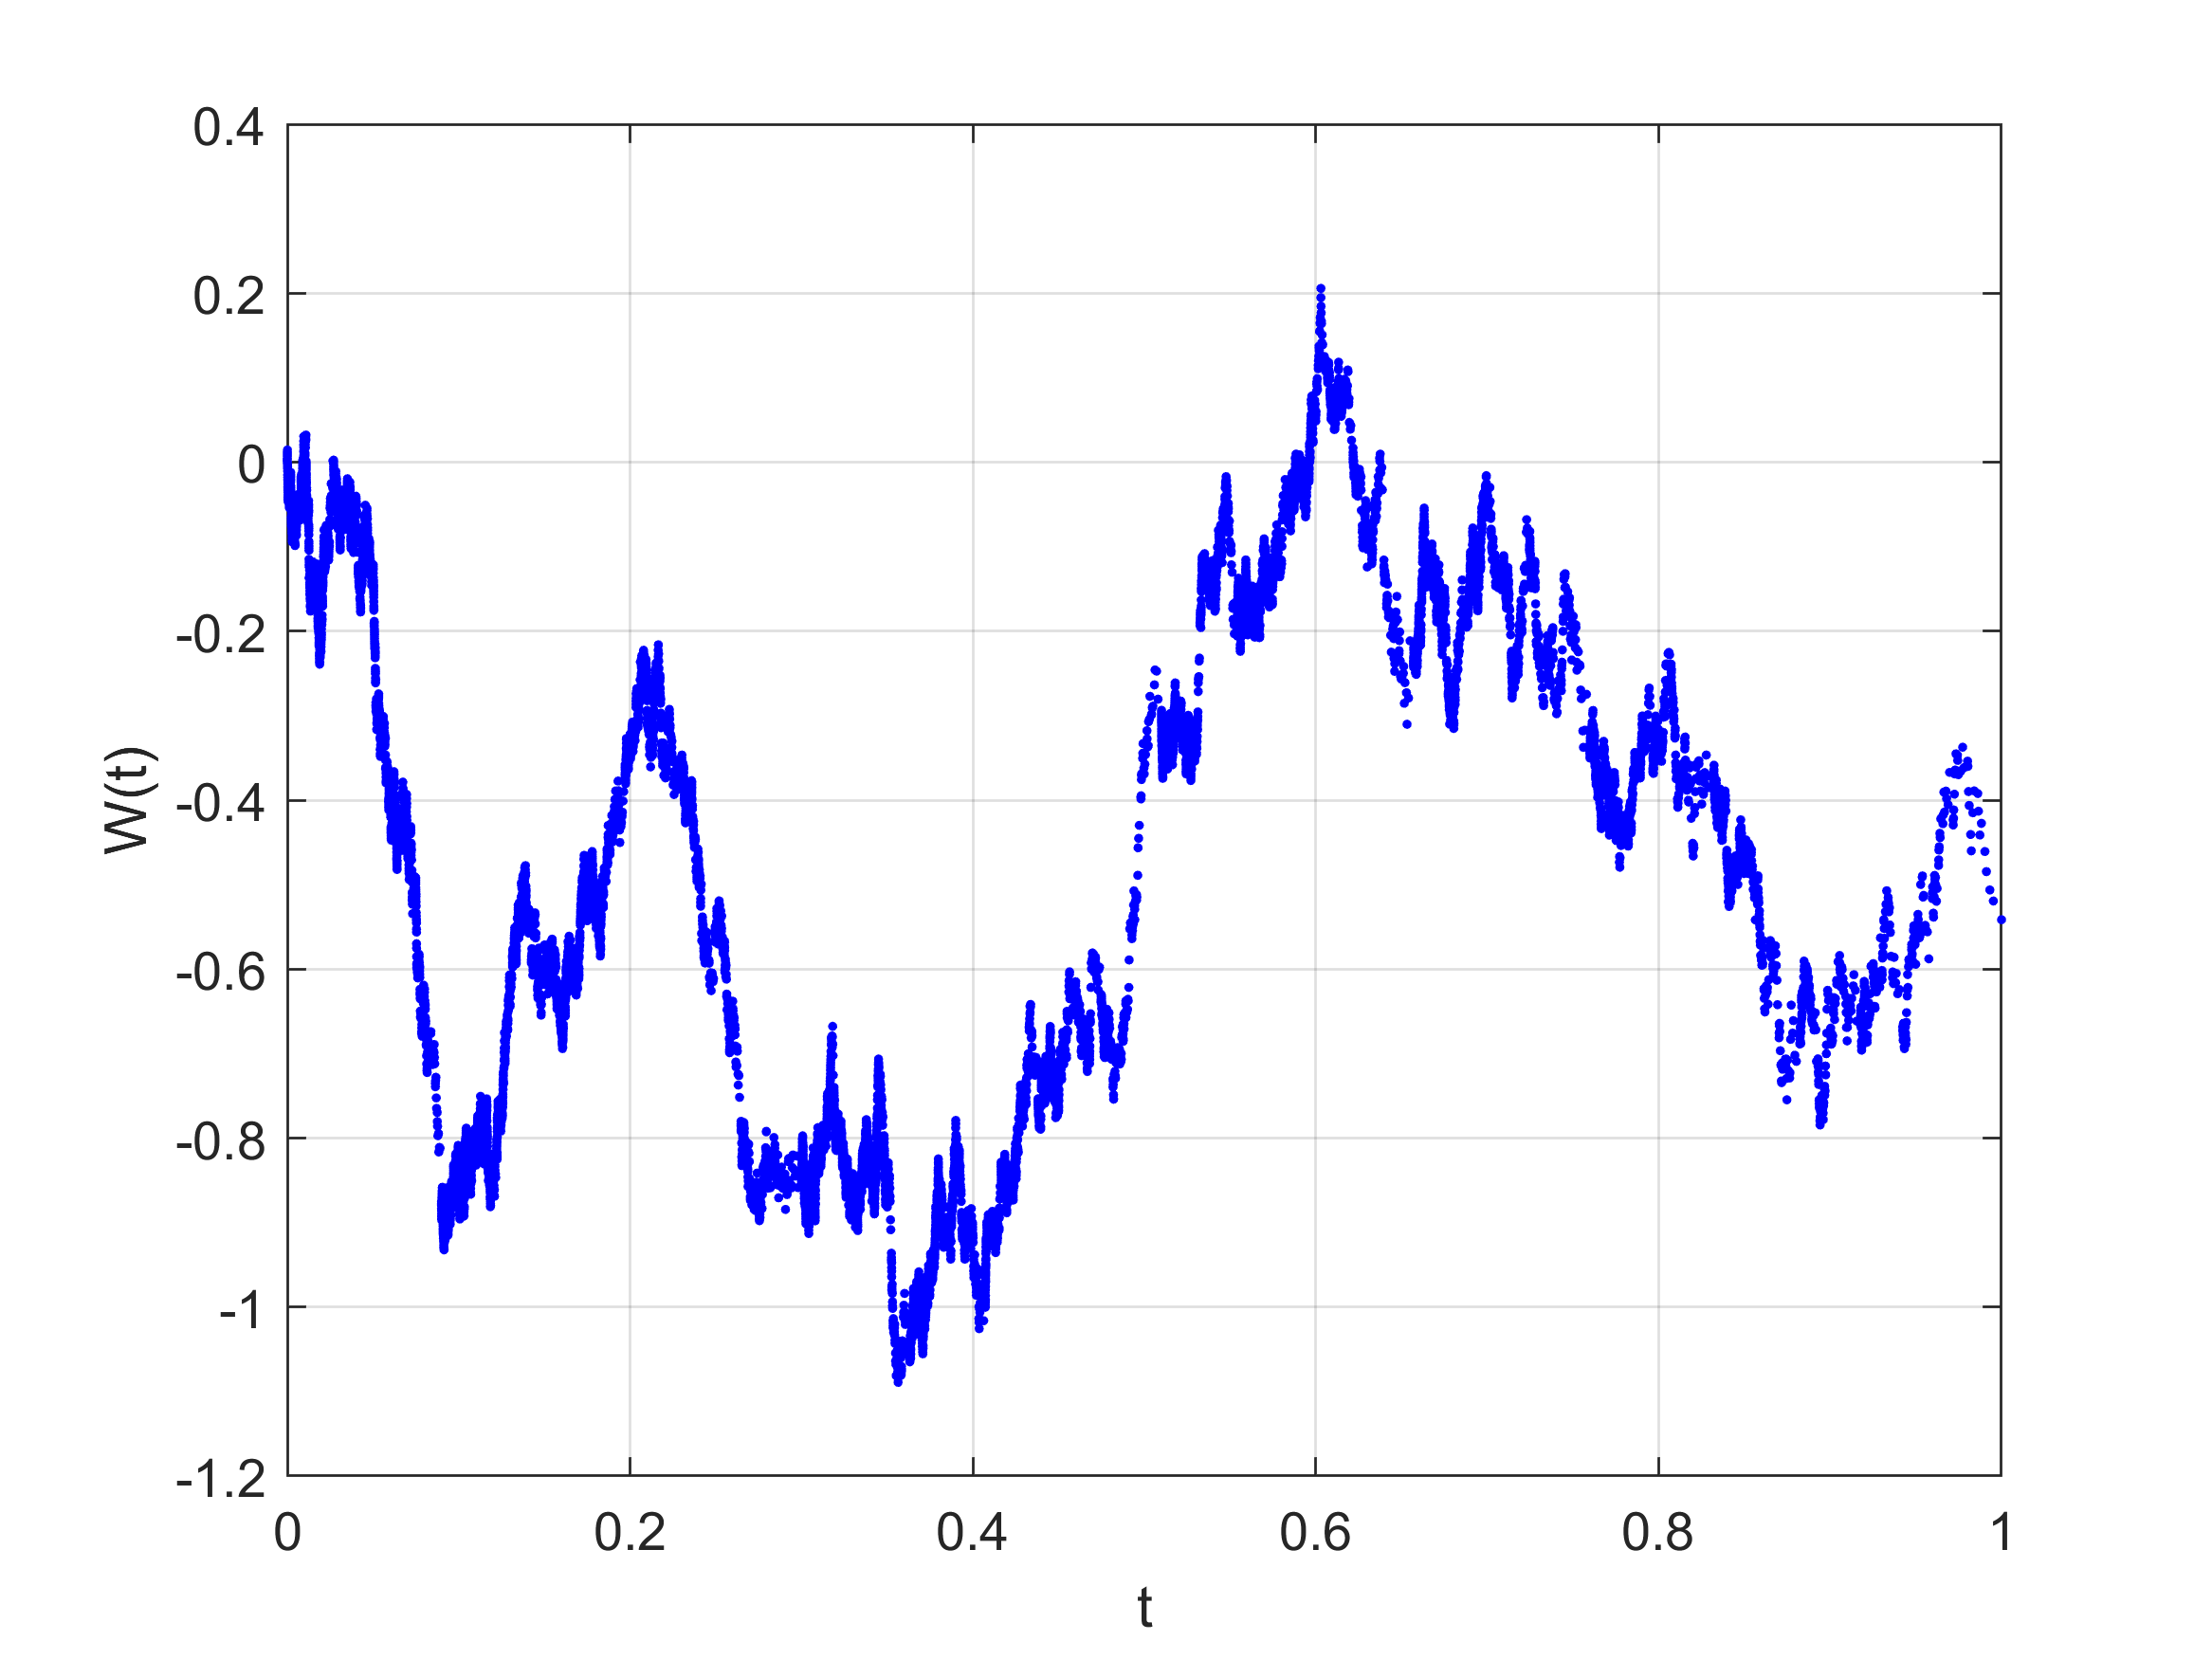
\includegraphics[width=0.6\textwidth]{../code/Task_9/pict/w_15_3_ex.png}
		\caption{Винеровский процесс с параметрами $n = 15, \alpha = 0.3$.}
    \end{figure}
	
\newpage	
\subsubsection{Пункт 2}
	\begin{definition}
		Cлучайный процесс $\{X_t |\, t\in T\}$ называется стационарным, если конечномерные
		распределения инвариантны относительно сдвига времени.
	\end{definition}
	
	Тогда из стационарности процесса Орншнейна-Уленбека следует,  что 
	$\E X_t = a, R(t,s)= R(|t-s|,0) =R(|t-s|)$.
	Без ограничения общности положим $a=0, \Var X_t = \sigma^2$, тогда:
	$$
		R(t,s) = \sigma^2 \rho(|t-s|), 
	$$
	где $\rho(|t-s|)=\rho(|t-s|,0)= \rho(t,s)$ --- коэффициент корреляции $X_t,X_s$.
	\newpage
	\begin{definition}
		Cлучайный процесс $\{X_t |\, t\in T\}$ называется марковским, если 
		$\forall t_1<t_2<\ldots<t_n \in T, B \in \mathcal{B}$ выполнено
		$$\mathbb{P}(X_{t_n} \in B | X_{t_1}, \ldots, X_{t_{n-1}}) = \mathbb{P}(X_{t_n} \in B | X_{t_{n-1}}).$$
	\end{definition}
	Отсюда следует, что $\rho(t+s)=\rho(t)\rho(s)$.
	\begin{theorem}
		Пусть функция $u(t)$ определена $\forall t > 0$ и ограничена на каждом конечном
		интервале. Если $u(t)$ удовлетворяет соотношению $u(t,s)=u(t)u(s)$, то или $u(t)=0, \forall t>0$,
		или $\exists \lambda > 0: u(t) = e^{-\lambda t}$.
	\end{theorem}
	Доказательство можно найти в $\cite{feller}$.
	\newline
	
	Если 	$\rho(t) \equiv 0 \Rightarrow \Cov (X_t,X_S) = 0$. 
	\newline В силу того, что процесс $\{X_t|\,t\in T\}$ --- гауссовский,
	то в данном случае $X_t$ независимы в совокупности. Это значит, что моделирование процесса 
	Орнштейна-Уленбека будет заключаться в генерации независимых случайных с распределением 
	$N(a,\sigma^2).$
	\newline
	
	Теперь рассмотрим случай, когда $\rho(s,t)=e^{-\lambda|t-s|}, \lambda>0 \Rightarrow 
		R(s,t) = \sigma^2e^{-\lambda|t-s|}.$ 
	\newline
	Найдем переходную плотность:
	$$
		p_{X_t}(x_1|X_s =x_2) = \dfrac{p_{X_t,X_s}(x_1, x_2)}	
															{p_{X_s}(x_2)}.
	$$
	Поскольку $\{X_t|\,t\in T\}$ --- гауссовский, то для $\hat x=(x_1,x_2)'$:
	$$
		\begin{gathered}
			p_{X_{t},X_{s}}(\hat{x}) = \dfrac{1}{2\pi \sqrt{|R|}} 
																	 e^{-\frac{1}{2}\hat{x}'R^{-1}\hat{x}}, \\
			p_{X_{s}}(x_2) = \dfrac{1}{\sqrt{2\pi} \sigma} 
																	 e^{-\frac{x_2^2}{2\sigma^2}}.											  
		\end{gathered}
	$$
	Ковариационная матрица $R$ имеет вид:
	$$
		R =  \begin{pmatrix} \sigma^2 & R(t,s) \\
											  R(t,s) & \sigma^2
				\end{pmatrix}, \quad 
		R^{-1} = \dfrac{1}{|R|} \begin{pmatrix} \sigma^2 & -R(t,s) \\
										 									-R(t,s) & \sigma^2
												\end{pmatrix}, \quad 
		|R| = \sigma^4 - R^2(t,s).										
	$$
	Сведя все воедино получим:
	$$
		p_{X_t}(x_1|X_s =x_2)  = \dfrac{1}{ \sqrt{ 2\pi \sigma^2 (1-e^{-2\lambda|t-s|}) }}
													\exp \left\{ \dfrac{\left( x_1 - x_2 e^{-\lambda|t-s|} \right)^2}
																				{2\sigma^2 (1-e^{-2\lambda|t-s|}) }
															\right \}.
	$$
	Таким образом: 
	$$
		X_t \sim N(x_2 e^{-\lambda|t-s|}, \sigma^2 (1-e^{-2\lambda|t-s|}) ) 
	$$
	\newpage
	Для непосредственного моделирования процесса расссмотрим случайные величины $X_{t_1},X_{t_2}$ 
	и найдем условную плотность:
	$$
		p_{X_t}(x|X_{t_1} = x_1, X_{t_2} = x_2) = \dfrac{p_{X_{t_1},X_t,X_{t_2}}(x_1, x, x_2)}
																						{p_{X_{t_1},X_{t_2}}(x_1, x_2)},
	$$
	но в данном случае $\alpha = 0.5$, т.е. $t=(t_1+t_2)\slash 2.$
	\newline
	Обозначим $\bar{x} = (x_1,x, x_2)'$ и $\hat{x} = (x_1,x_2)'$, тогда плотности распределения этих векторов 
	будут равны:
	$$
		\begin{gathered}
			p_{X_{t_1},X_t,X_{t_2}}(\bar{x}) = \dfrac{1}{(2\pi)^{\frac{3}{2}} \sqrt{|R_1|}} 
																			e^{-\frac{1}{2}\bar{x}'R_1^{-1}\bar{x}},	 \\ 		
			p_{X_{t_1},X_{t_2}}(\hat{x}) = \dfrac{1}{2\pi \sqrt{|R_2|}} 
																			e^{-\frac{1}{2}\hat{x}'R_2^{-1}\hat{x}},				
		\end{gathered}
	$$
	где $R_1, R_2$ --- соответствующие матрицы ковариаций. Вспомним, что 
		$R(t,s) = \sigma^2e^{-\lambda|t-s|}$, поэтому:
	$$
		R_1 = \sigma^2 \begin{pmatrix} 	1 & e^{-\lambda(t-t_1)} & e^{-\lambda(t_2-t_1)} \\
															 e^{-\lambda(t-t_1)} & 1 & e^{-\lambda(t_2-t)} \\
															 e^{-\lambda(t_2-t_1)} & e^{-\lambda(t_2-t)} & 1 \end{pmatrix}, \quad
		R_2 = \sigma^2 \begin{pmatrix} 1 & e^{-\lambda(t_2-t_1)} \\ e^{-\lambda(t_2-t_1)} & 1 \end{pmatrix}.
	$$
	Используя символьные вычисления $Matlab$ получим окончательно:
	$$
		X_t \sim N\left( 
									(x_1+x_2)\dfrac{e^{-\frac{\lambda(t_2-t_1)}{2}}}{1+e^{-\lambda(t_2-t_1)}},
									\sigma^2 \dfrac{1-e^{-\lambda(t_2-t_1)}}{1+e^{-\lambda(t_2-t_1)}}
						 \right).
	$$	
	В качестве начальных значений возьмем: $X_0 \sim N(0,\sigma^2), 
																			X_1 \sim N(x_0e^{-\lambda T},\sigma^2(1-e^{-2\lambda T})).$	
	\begin{figure}[h!]
		\centering
		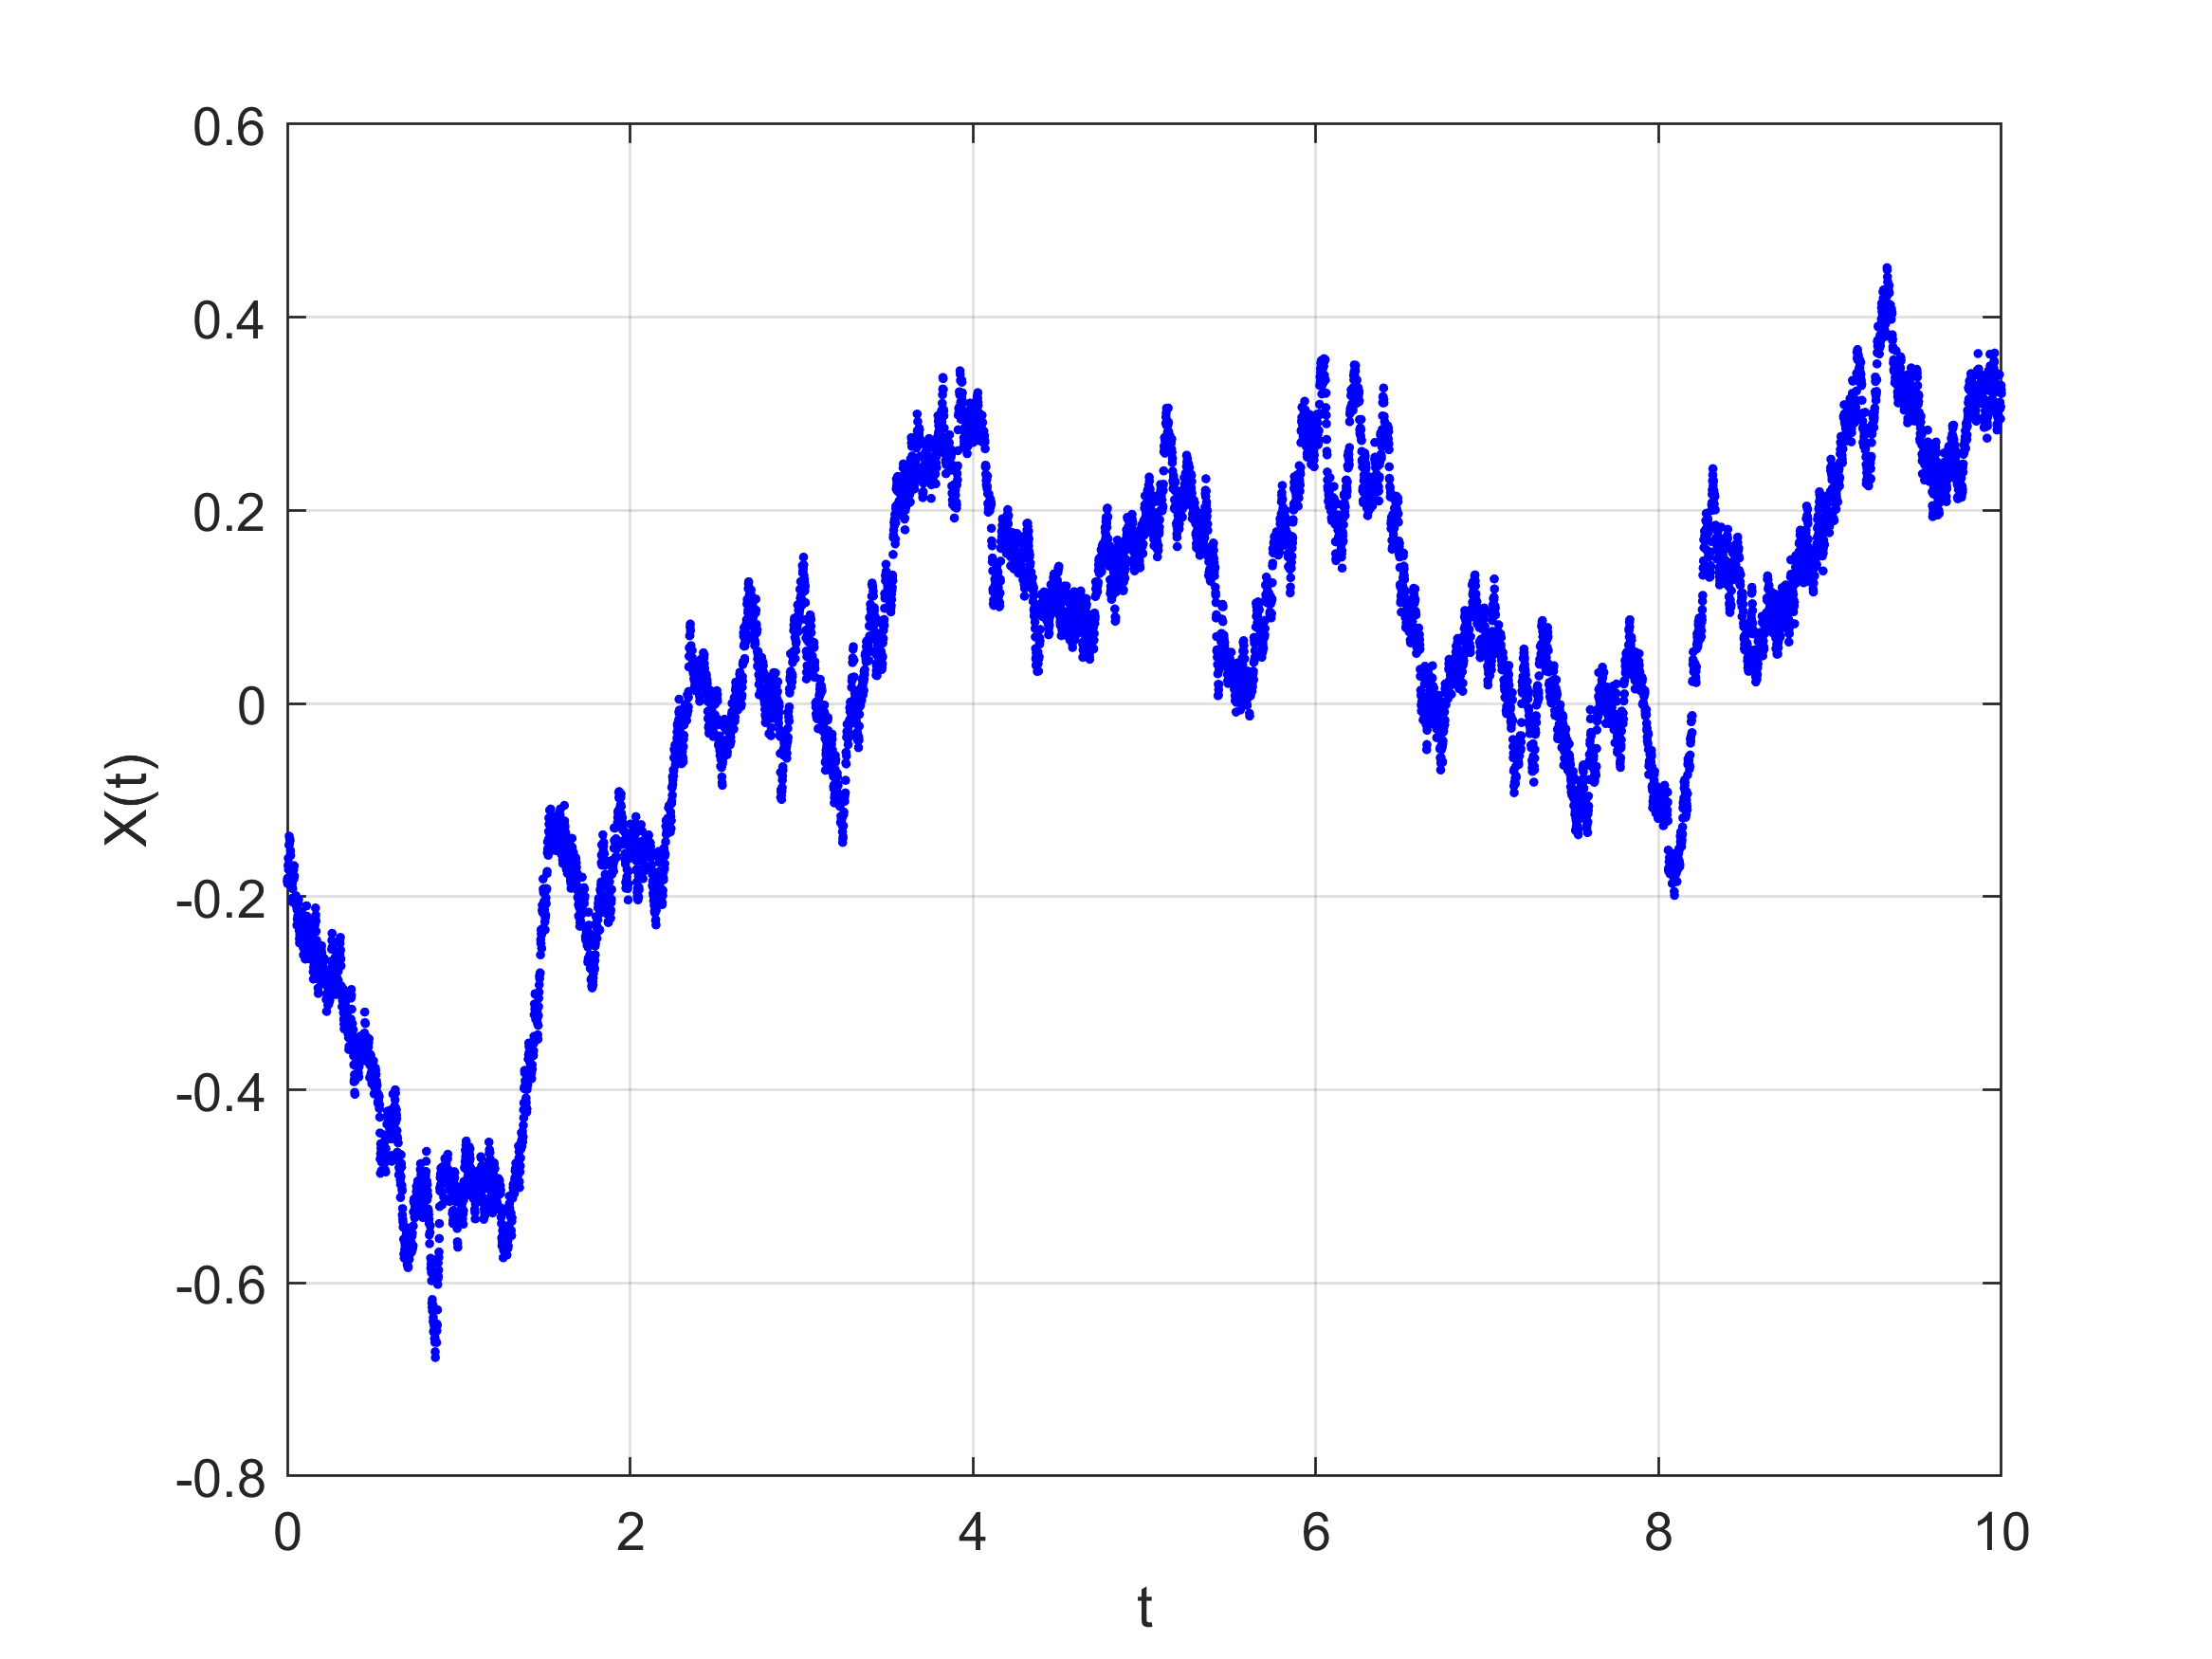
\includegraphics[width=0.6\textwidth]{../code/Task_9/pict/ou_13_1_20_ex.png}
		\caption{Процесс Орнштейна-Уленбека с параметрами $n = 13, \lambda = 1, \sigma = 0.2$. }
    \end{figure}
    \newpage
    \begin{figure}[h!]
		\centering
		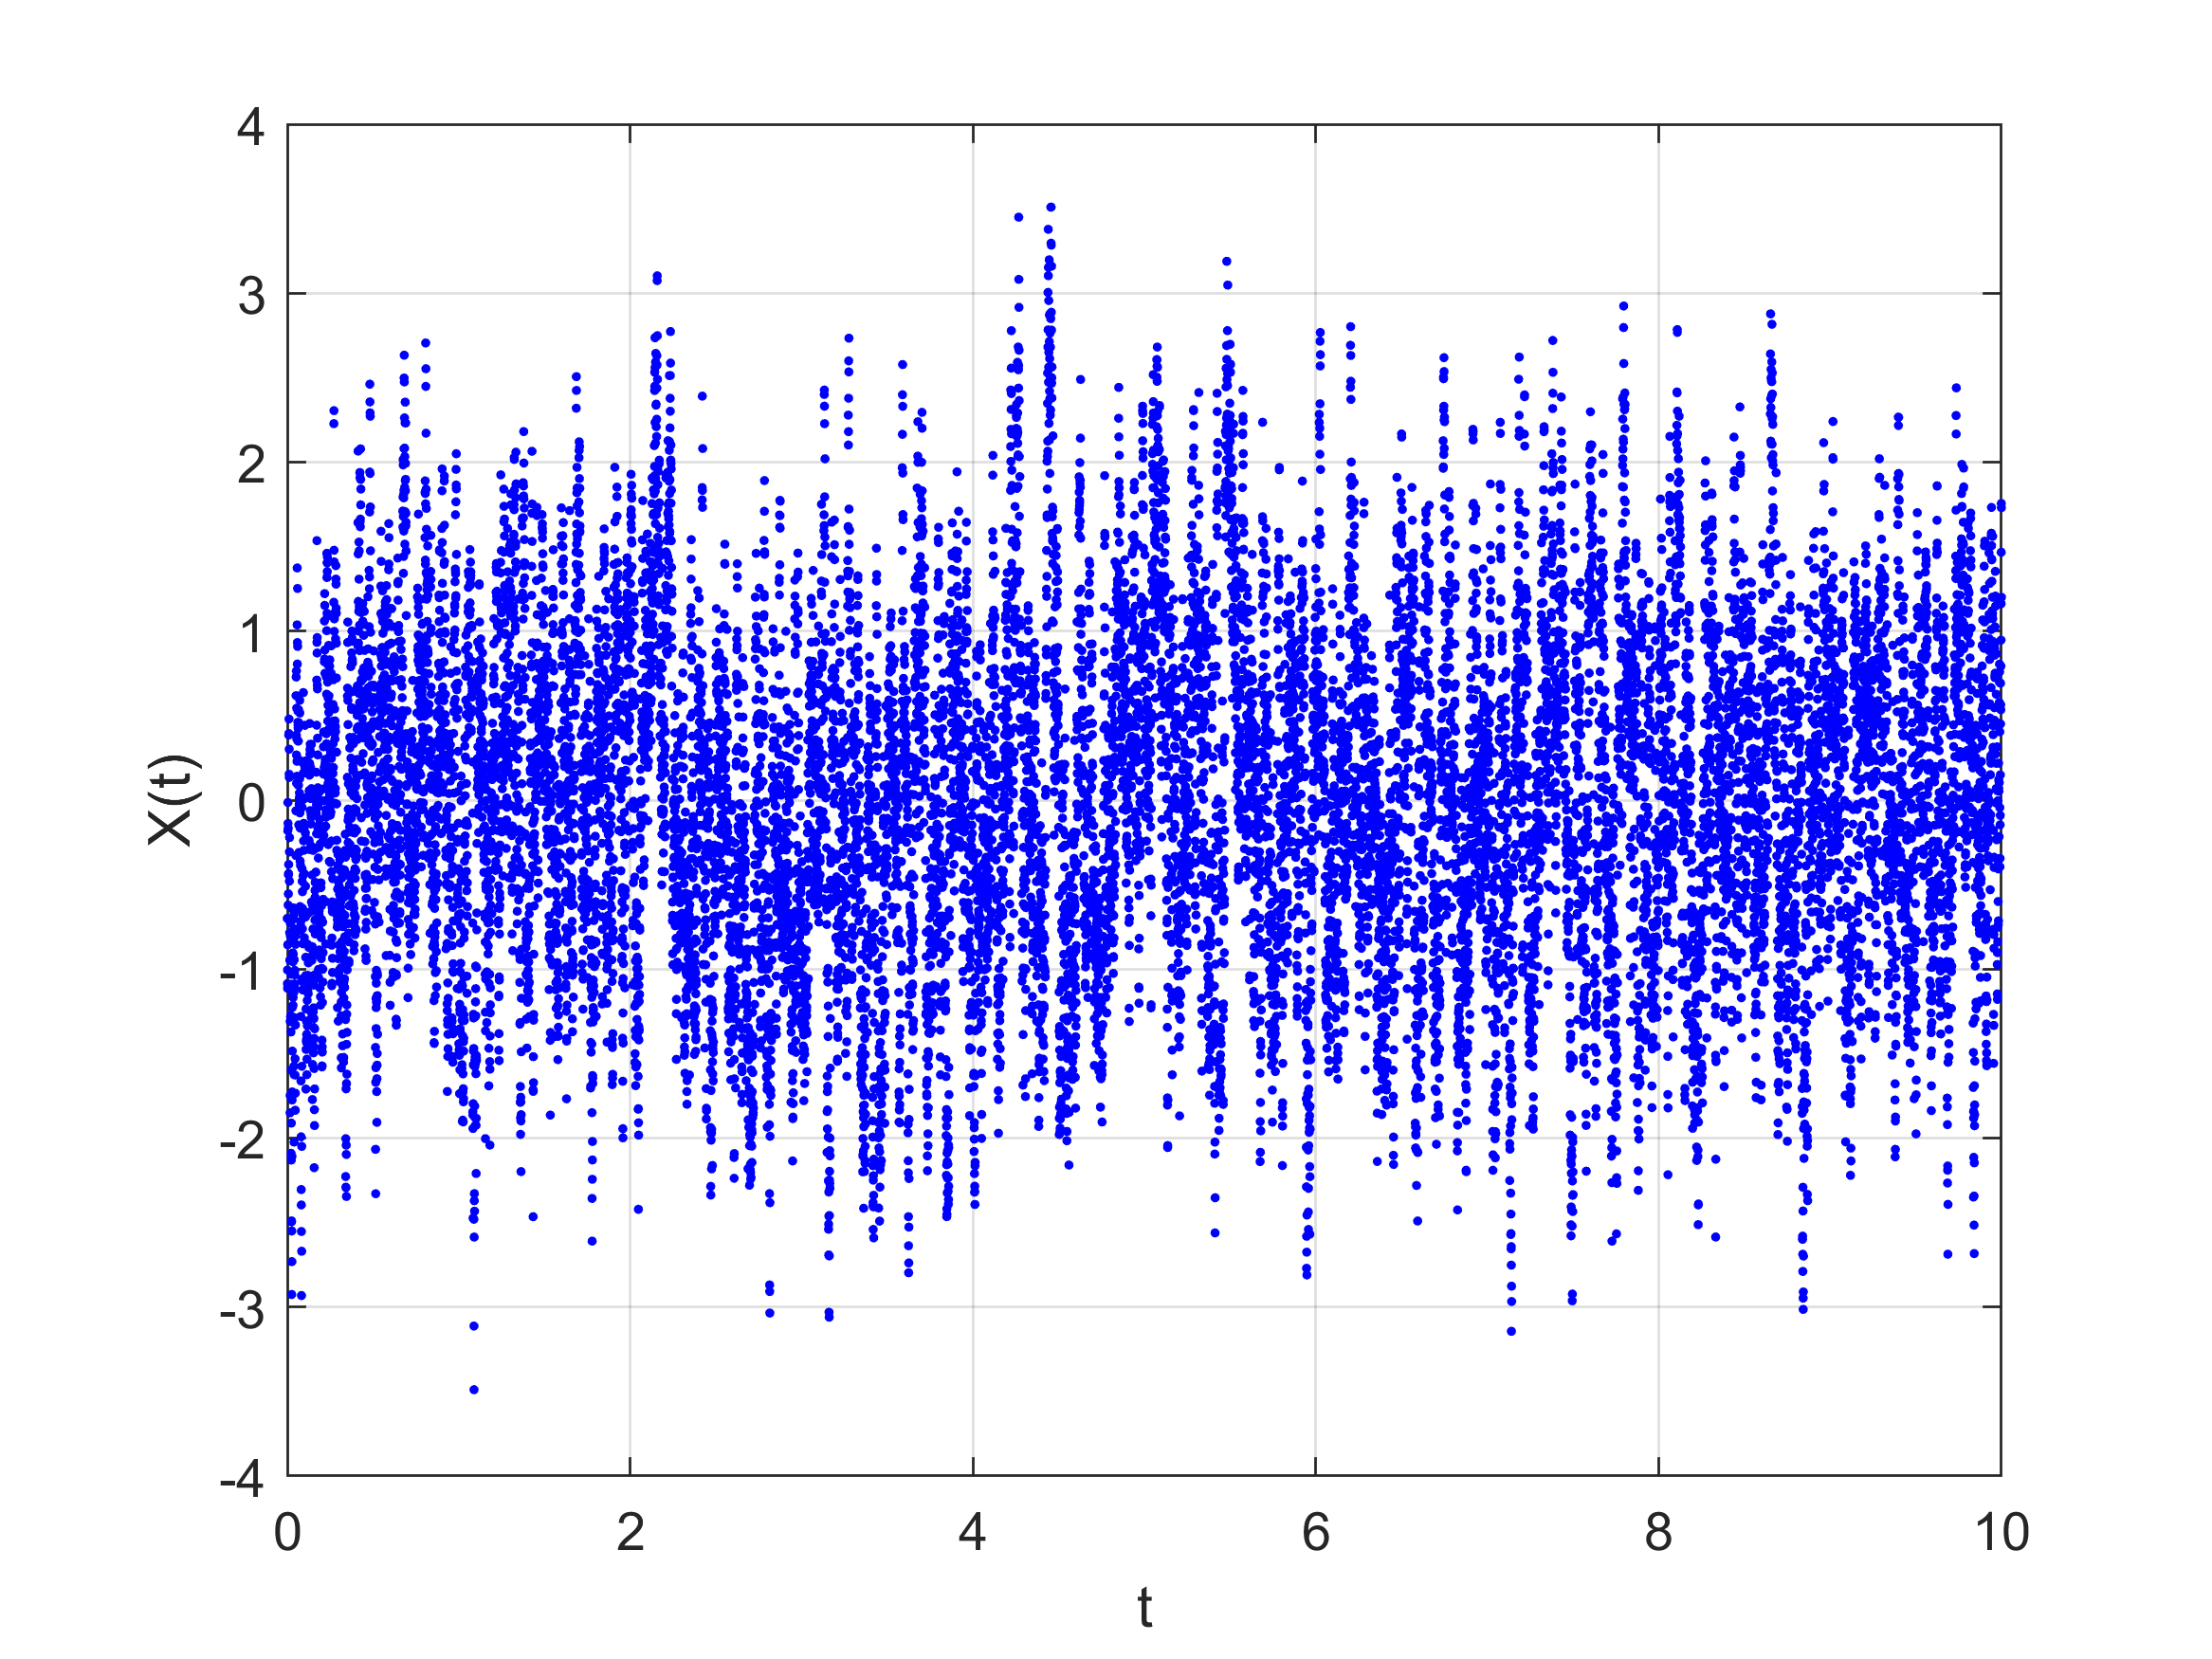
\includegraphics[width=0.6\textwidth]{../code/Task_9/pict/ou_14_100_1_ex.png}
		\caption{Процесс Орнштейна-Уленбека с параметрами  $n = 14 \lambda = 100, \sigma = 1$.}
    \end{figure}
     \begin{figure}[h!]
		\centering
		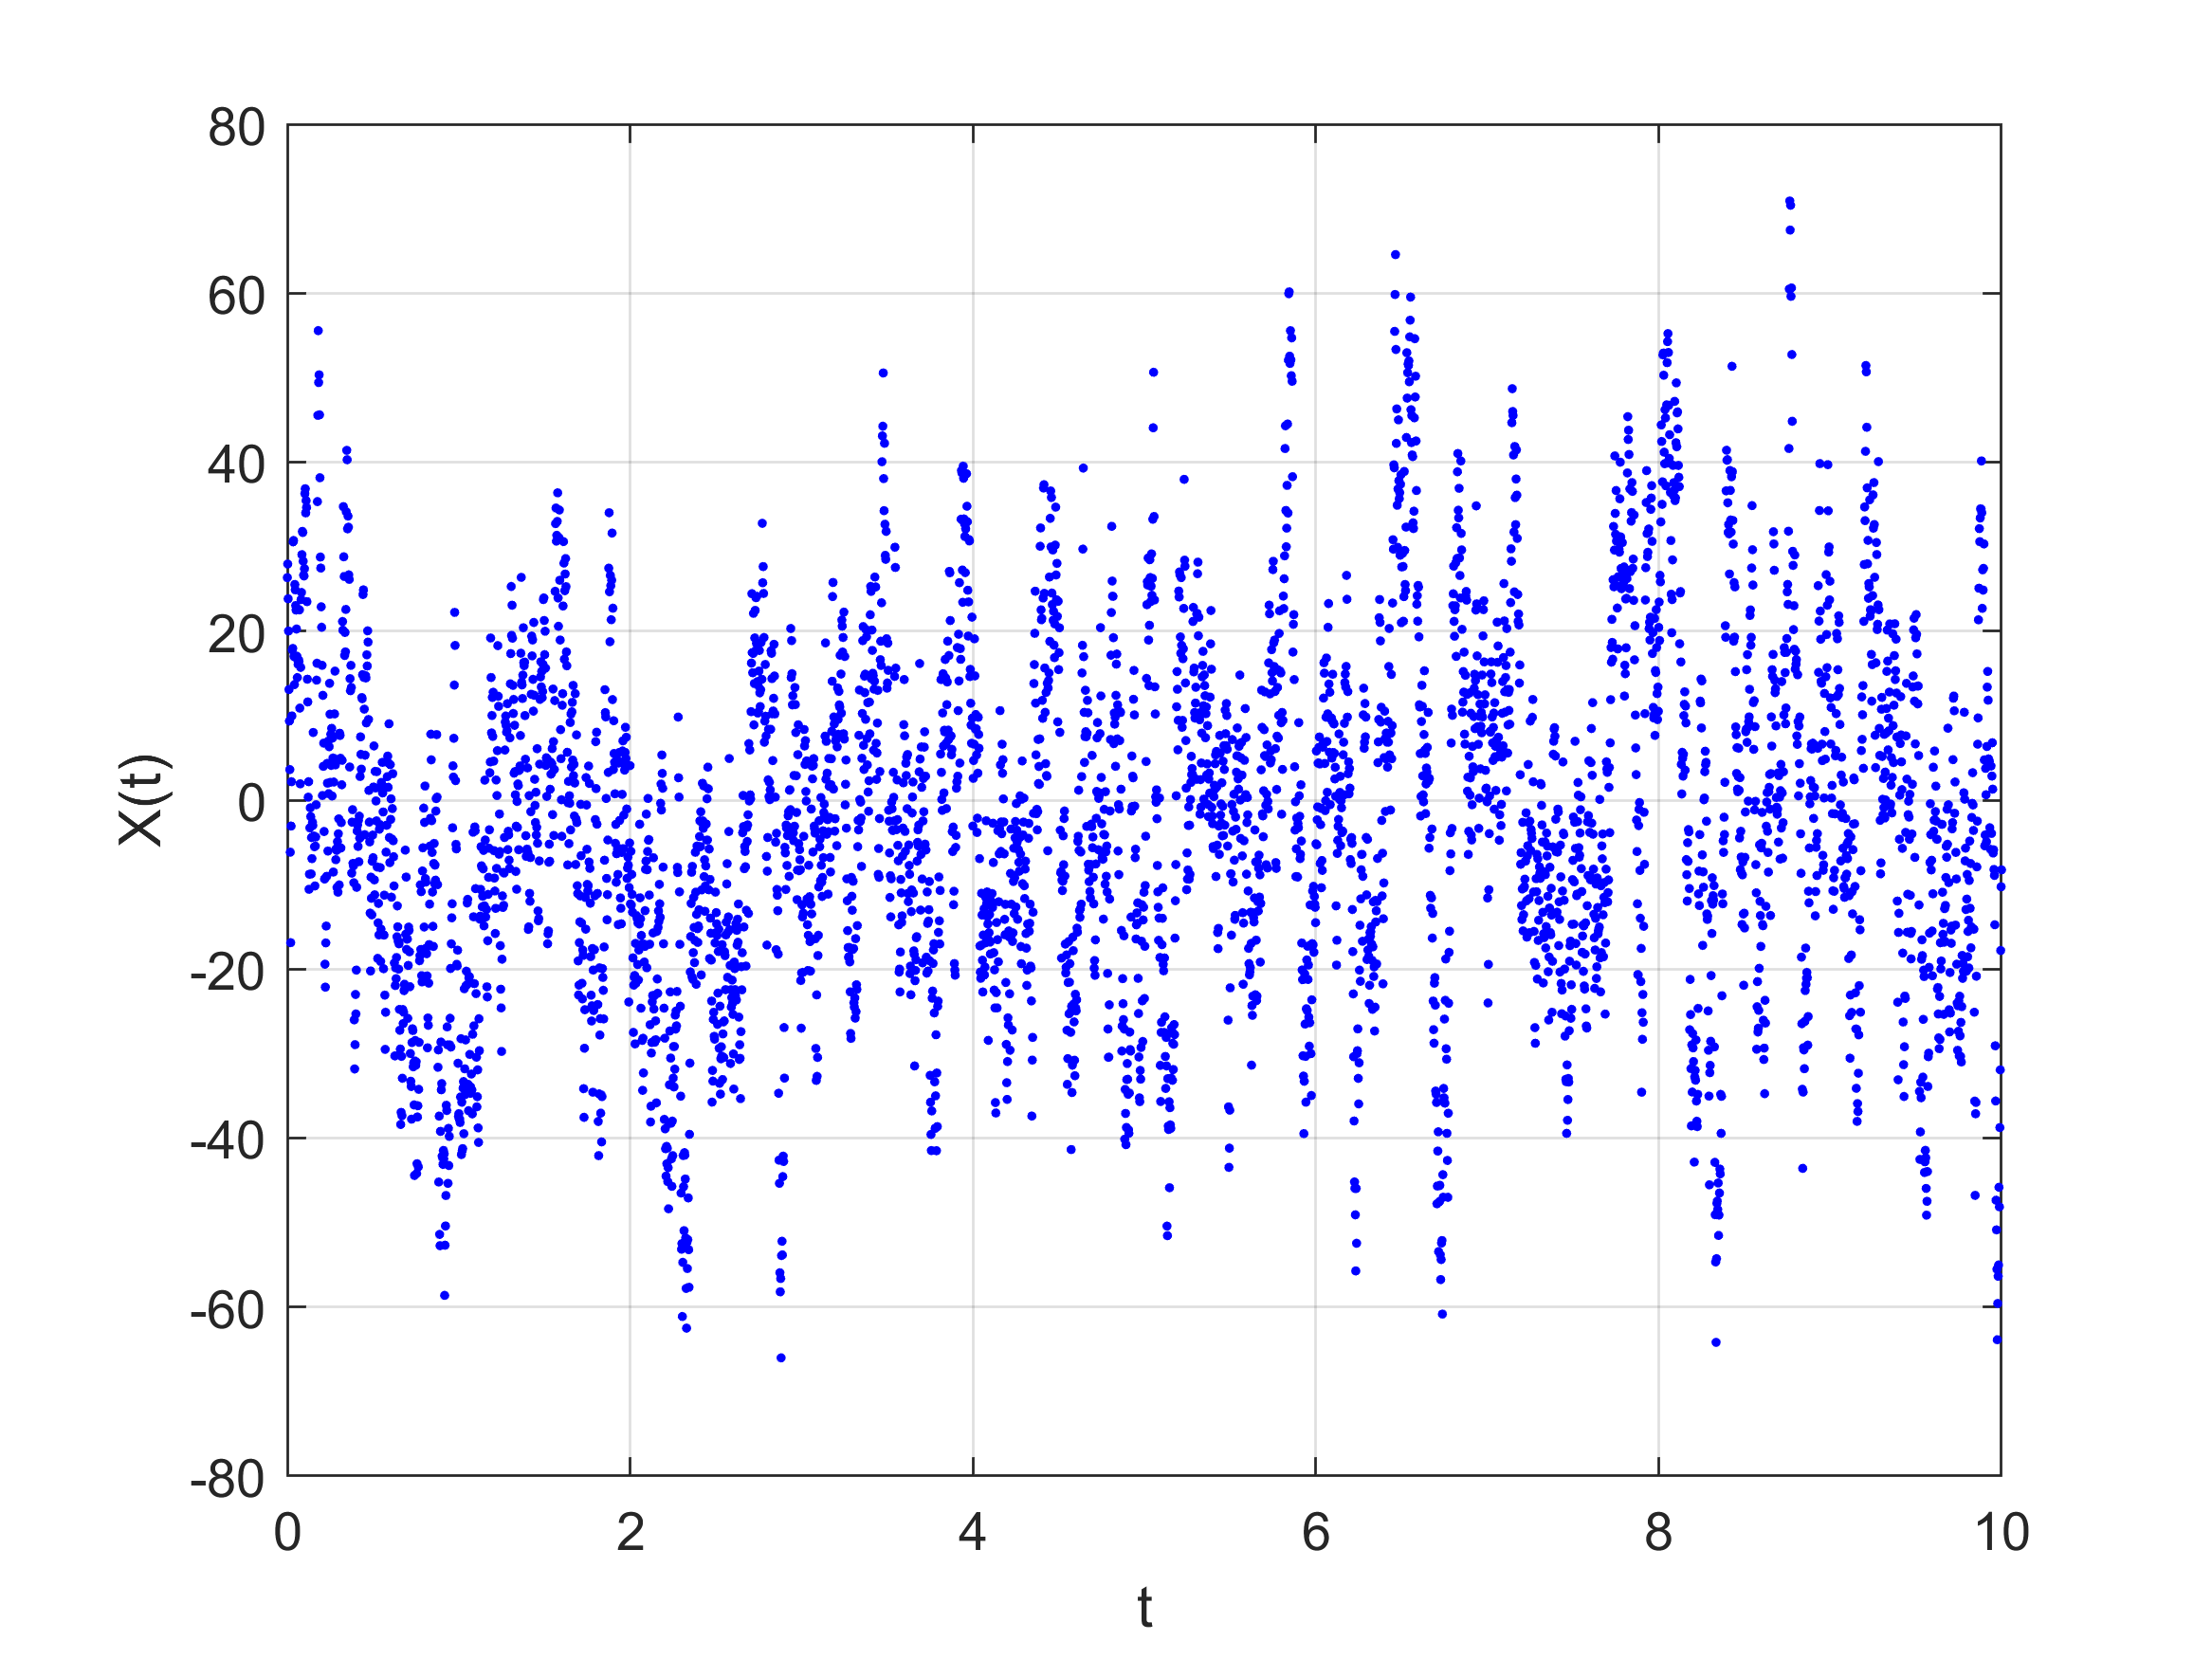
\includegraphics[width=0.6\textwidth]{../code/Task_9/pict/ou_12_30_20_ex.png}
		\caption{Процесс Орнштейна-Уленбека с параметрами  $n = 14 \lambda = 30, \sigma = 20$.}
    \end{figure}
\newpage
\section{Задание 10}

\subsection{Постановка задачи}
	Провести фильтрацию одномерного процесса Орнштейна- Уленбека:
    \begin{enumerate} 
        \item Используя генератор белого шума, добавить случайную ошибку с известной дисперсией к реализации 
        		процесса Орнштейна- Уленбека. 
        \item При помощи одномерного фильтра Калмана оценить траекторию процесса по зашумленному сигналу.
        		Параметры процесса и белого шума считать известными. 
        \item Расмотреть случай, когда шум
        	\begin{itemize}
        		\item Является гауссовским. 
        		\item Имеет распределение Коши.
        	\end{itemize}
    \end{enumerate}
\subsection{Решение задачи}

	\begin{definition}
		Дискретным белым шумом называется последовательность $\xi_1,\ldots,\xi_n,\ldots$ независимых 
		одинаково распределенных случайных величин.
	\end{definition}
	Рассматриваемый нами процесс Орншейна-Уленбека --- это марковский процесс, 
	поэтому можно определить совместную плотность по всем моментам времени:
	$$
		\begin{gathered}
			p(x_k, \ldots,x_0) = p(x_k|x_{k-1},\ldots,x_0)\cdot  p(x_{k-1}|x_{k-2},\ldots,x_0)\cdot
				 \ldots \cdot  p(x_1|x_0) \cdot p(x_0) = \\
				 = \text{\{в силу марковского свойства\}} =  p(x_k|x_{k-1})\cdot p(x_{k-1}|x_{k-2}) 
				 	\ldots \cdot  p(x_1|x_0) \cdot p(x_0)
		\end{gathered}
	$$
	Рассмотрим соотношение:
	\begin{equation}
		x_{k+1} = f(x_k)+w(k), \label{eq_1}
	\end{equation}
	 где $w(k)$ - случайная помеха, $x_k, w(k)$ независимы и имеют гауссовское распределение, 
	 $f(x_k) = \E (x_{k+1}|x_k)$. 
	 \newline При сделанных предположениях условное математическое ожидание 
	 $\E (x_{k+1}|x_k)$ линейно по $x_k$. Тогда ($\ref{eq_1}$) переходит в уравнение:
	 $$ x_{k+1} = A_k x_k + w_k.$$
	 Поскольку случайные величины гауссовские, то для их полного описания достаточно знать 
	 первые и вторые моменты.
	 Обратимся к $\cite{th_ident}$ и выпишем каноническую систему для нахождения
	 исходного процесса с помощью фильтра Калмана со схемой <<шагаем-меряем>>:
	 \begin{equation}
	 	\begin{cases}
	 		x_{k+1} = A_k x_k + w_k, \quad k = \overline{0,N-1}, \\
	 		y_{k} = C_k x_k + v_k, \qquad k = \overline{0,N}, 
	 	\end{cases} \label{kalm_sys}
	\end{equation}
	где $\{x_0, w_0, \ldots w_{N-1}, v_0, \ldots v_N\}$ независимы в совокупности, 
	$Y_{N}= (y_0, \ldots, y_{N}) $ --- наблюдения, $X_{N}= (x_0, \ldots, x_{N}) $--- исходный процесс, 
	который нужно найти.
	\newpage
	Введем обозначения $\E x_0 = \bar{x}_0, \Var x_0= S, 
	\E w_k = \E v_k = 0, \Var w_k = M_k, \Var v_k= N_k$ и выпишем систему, реализующую 
	фильтр Калмана: 
	\begin{equation}
		\begin{cases}
			x_{k+1|k} = A_k x_{k|k}, \\
			x_{k|k}  = x_{k|k-1} + R_{k|k-1} C_k^T(C_k R_{k|k-1}C_k^T + N_k)^{-1}(y_k - C_k x_{k|k-1}), \\
			R_{k+1|k} = A_k R_{k|k} A_k^T + M_k,\\
			R_{k|k} = R_{k|k-1} - R_{k|k-1} C_k^T(C_k R_{k|k-1}C_k^T + N_k)^{-1}C_k R_{k|k-1}, \\
			x_{0|-1} = x_0,\\ 
			R_{0|-1} = S.
		\end{cases} \label{kalm}
	\end{equation}
	Так как рассматриваемая задача одномерная, то все коэффициенты сисемы ($\ref{kalm}$) будут скалярами.
	Определим их. Рассмотрим уравнение для наблюдения:
	$$y_{k} = x_{k} + v_k,$$
	где $v_k$ - это белый шум с дисперсией $\sigma_2 \Rightarrow N_k = \sigma_2^2, C_k =1.$
	Исходя из системы ($\ref{kalm_sys}$) получatм: 
	$$
		\begin{gathered}
			\Var x_{k+1} = A_k^2\Var x_k + \Var w_k = A_k^2V_k+ M_k, \\
			\Cov (x_{k+1},x_k) = \E (x_{k+1},x_k) - \E x_{k+1}\E x_{k} = A_k (\E x_k^2 - (\E x_k)^2)
			= A_k\Var x_k = A_kV_k.
		\end{gathered}
	$$
	Из задачи 9 мы знаем, что ковариационная функция для процесса Орнштейна-Уленбека
	 с параметрами $\lambda, \sigma_1$
	имеет вид:
	$$
		R(t,s) = \sigma_1^2e^{-\lambda|t-s|} \Rightarrow
			\begin{cases}
				\sigma_1^2 = V_k, \\
				\sigma_1^2e^{-\lambda\Delta t} = A_k V_k, \quad \Delta t = t_{i+1}-t_i, \\ 
				\sigma_1^2 = A_k^2V_k+ M_k,
			\end{cases}
	$$
 	Решив эту систему получим: $A_k=e^{-\lambda\Delta t}, 
 			V_k = \sigma_1^2, M_k =  \sigma_1^2(1-e^{-2\lambda\Delta t}). $
 	\newline
	Выделим повторяющуюся компоненту:
	$$
		h =  R_{k|k-1}(R_{k|k-1} + \sigma_2^2)^{-1}. 
	$$
	Перепишем систему ($\ref{kalm}$) для исследуемого процесса:
	\begin{equation}
		\begin{cases}		
			x_{k|k}  = (1-h) x_{k|k-1} + h y_k, \\
			R_{k|k} = (1- h) R_{k|k-1}, \\
			h =  R_{k|k-1}(R_{k|k-1} + \sigma_2^2)^{-1}, \\
			x_{k+1|k} = e^{-\lambda\Delta t} x_{k|k}, \\
			R_{k+1|k} = e^{-2\lambda\Delta t} R_{k|k} + \sigma_1^2(1-e^{-2\lambda\Delta t}),\\
			x_{0|-1} = 0,\\ 
			R_{0|-1} = \sigma_1^2.
		\end{cases} \label{kalm}
	\end{equation}
	Доверительный интервал задается уранением: $$x_k +k_{(1-\alpha)\slash 2}[-R_{k|k},R_{k|k}],$$ 
	где $\alpha$ --- уровень значимости, а $k_{(1-\alpha)\slash 2}$ --- квантиль нормального распределения.
\newpage
	Рассмотрим примеры работы программы.
	\begin{itemize}
		\item 	Случай, когда шум имеет гауссовское распределение:
					\begin{figure}[h!]
						\centering
						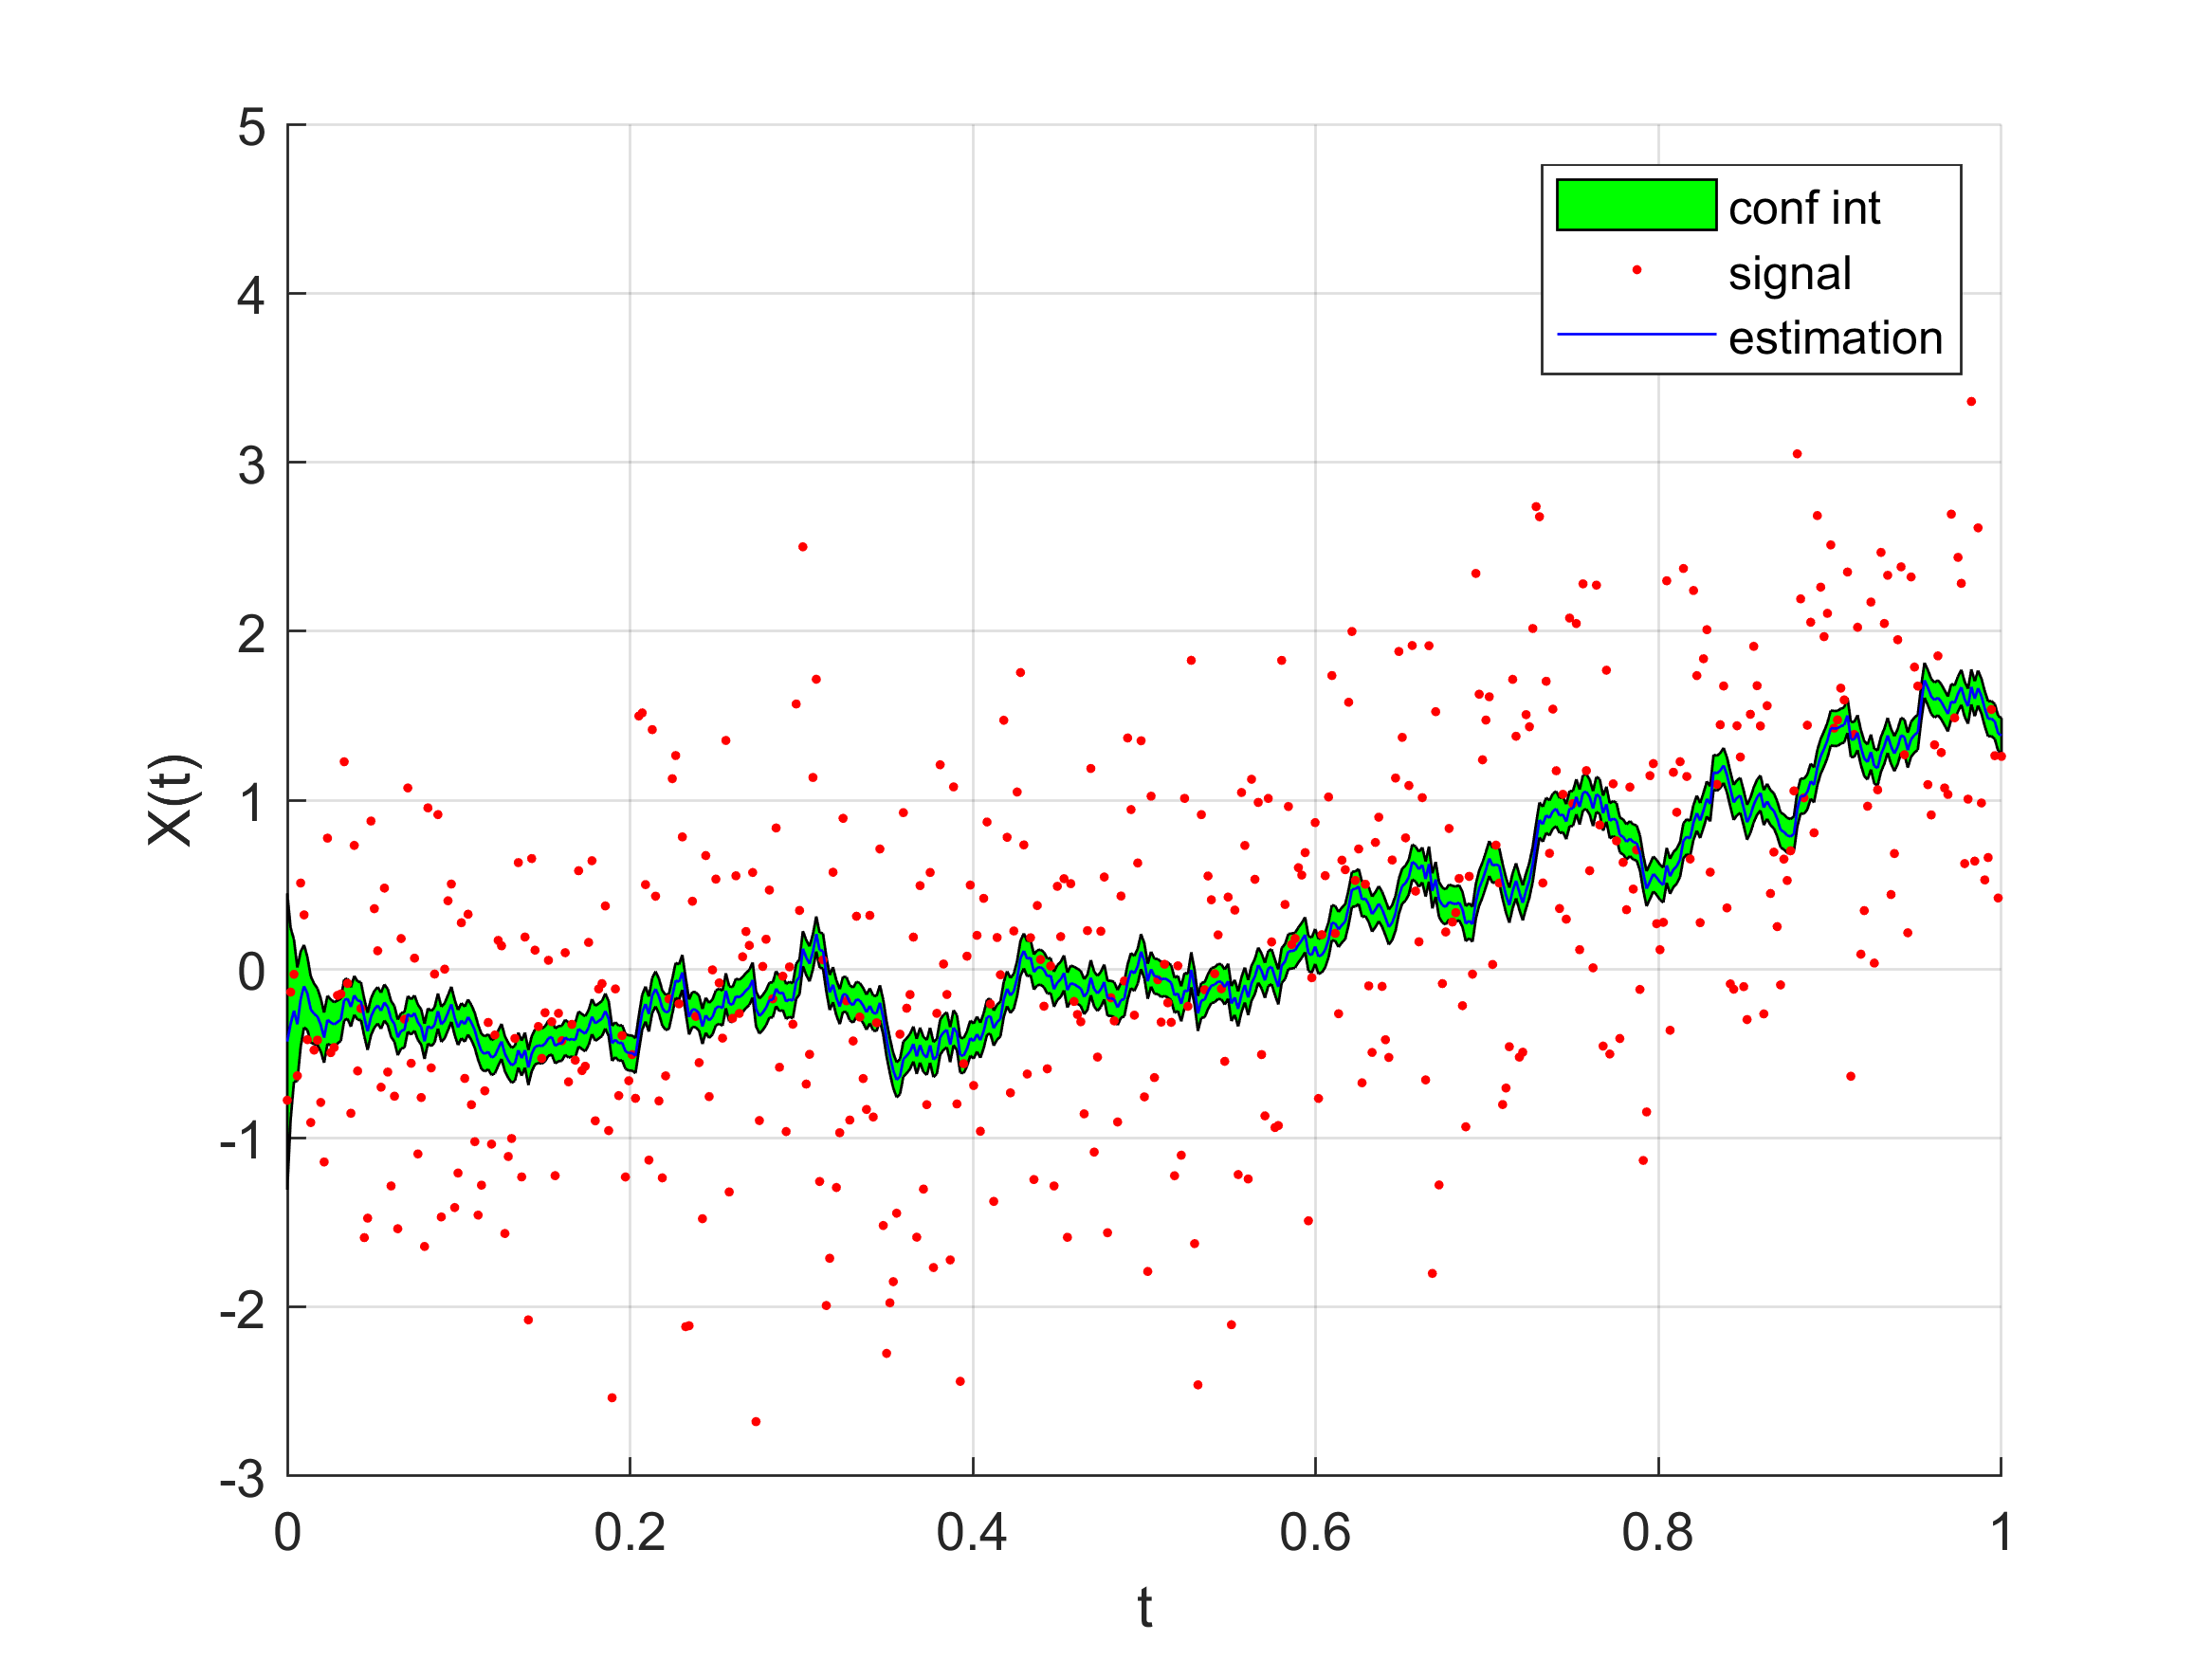
\includegraphics[width=0.6\textwidth]{../code/Task_10/pict/norm_1_1_90_ex.png}
						\caption{Процесс с параметрами $\lambda = 1,\sigma_1 = 1, \sigma_2 = 0.9, T = 1$.}
				    \end{figure}
				    \begin{figure}[h!]
						\centering
						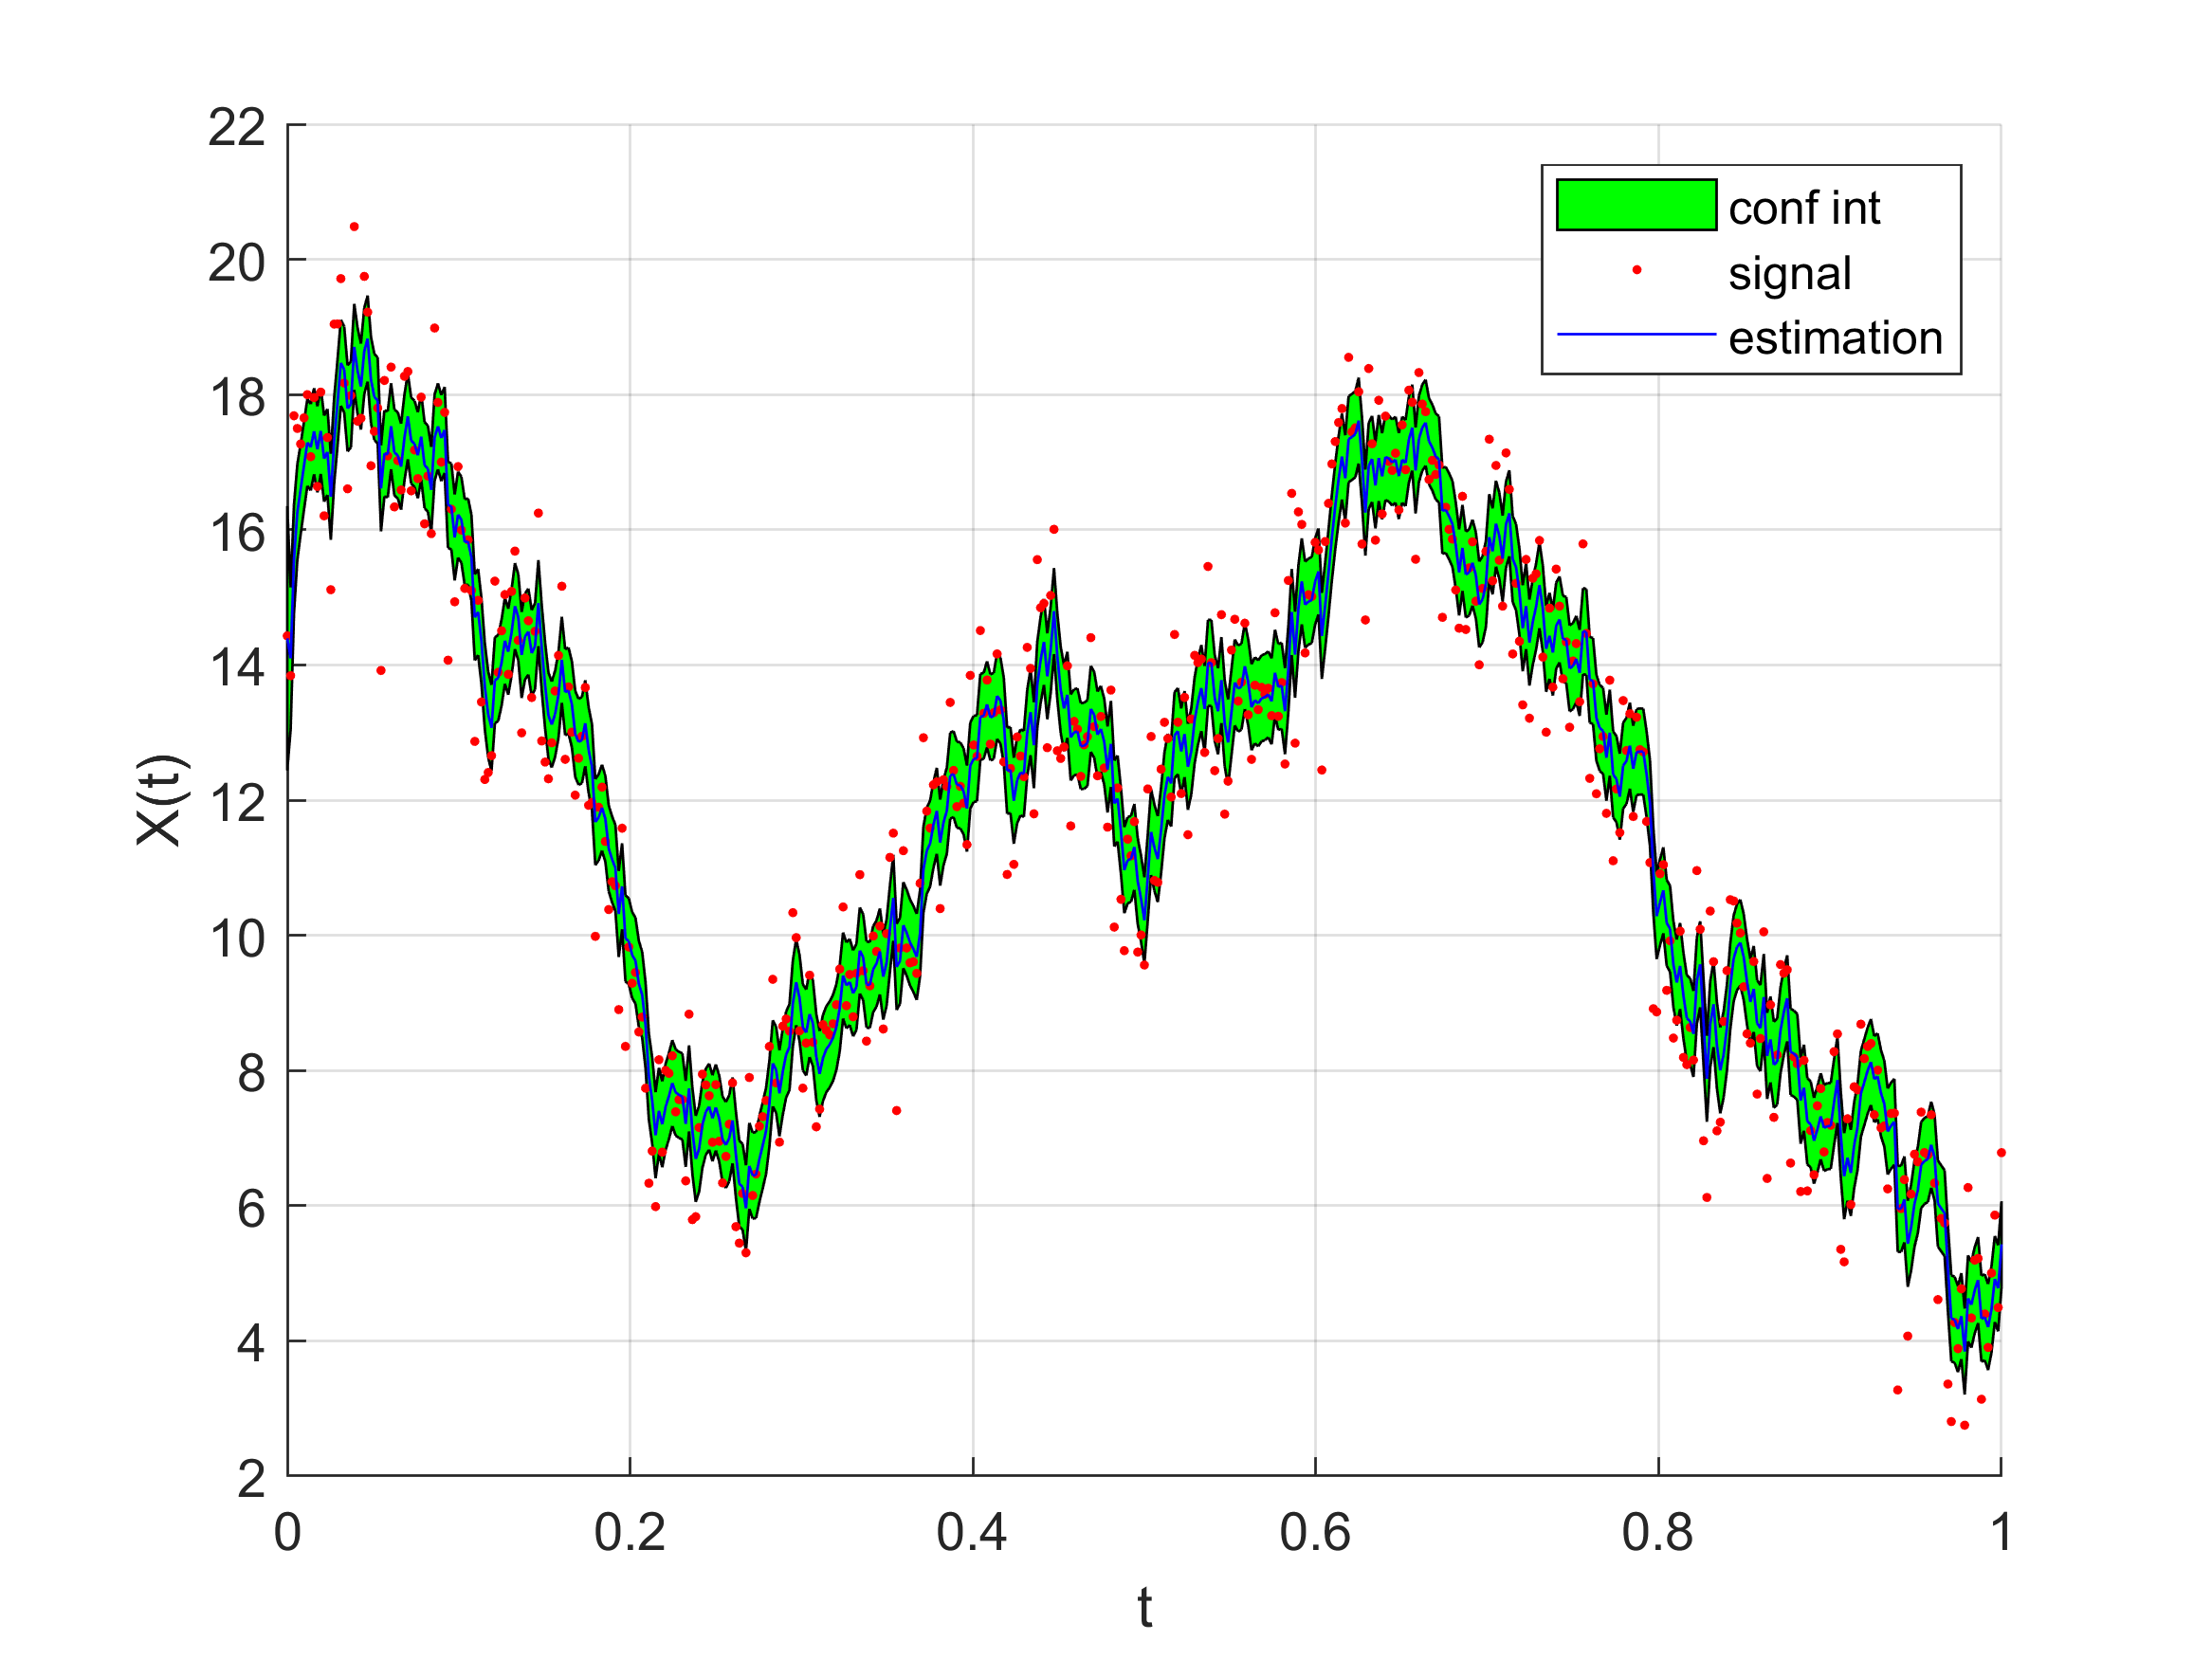
\includegraphics[width=0.6\textwidth]{../code/Task_10/pict/norm_20_1_10_ex.png}
						\caption{Процесс с параметрами $\lambda = 0.1,\sigma_1 = 20, \sigma_2 = 1, T = 1$.}
				    \end{figure}
				    
				   Как мы видим, на рисунках четко выделяется траектория исходного процесса, т.е. 
				   действительно произошла фильтрация.\newpage
	    \item 	Случай, когда шум имеет распределение Коши:
	    			\begin{figure}[h!]
						\centering
						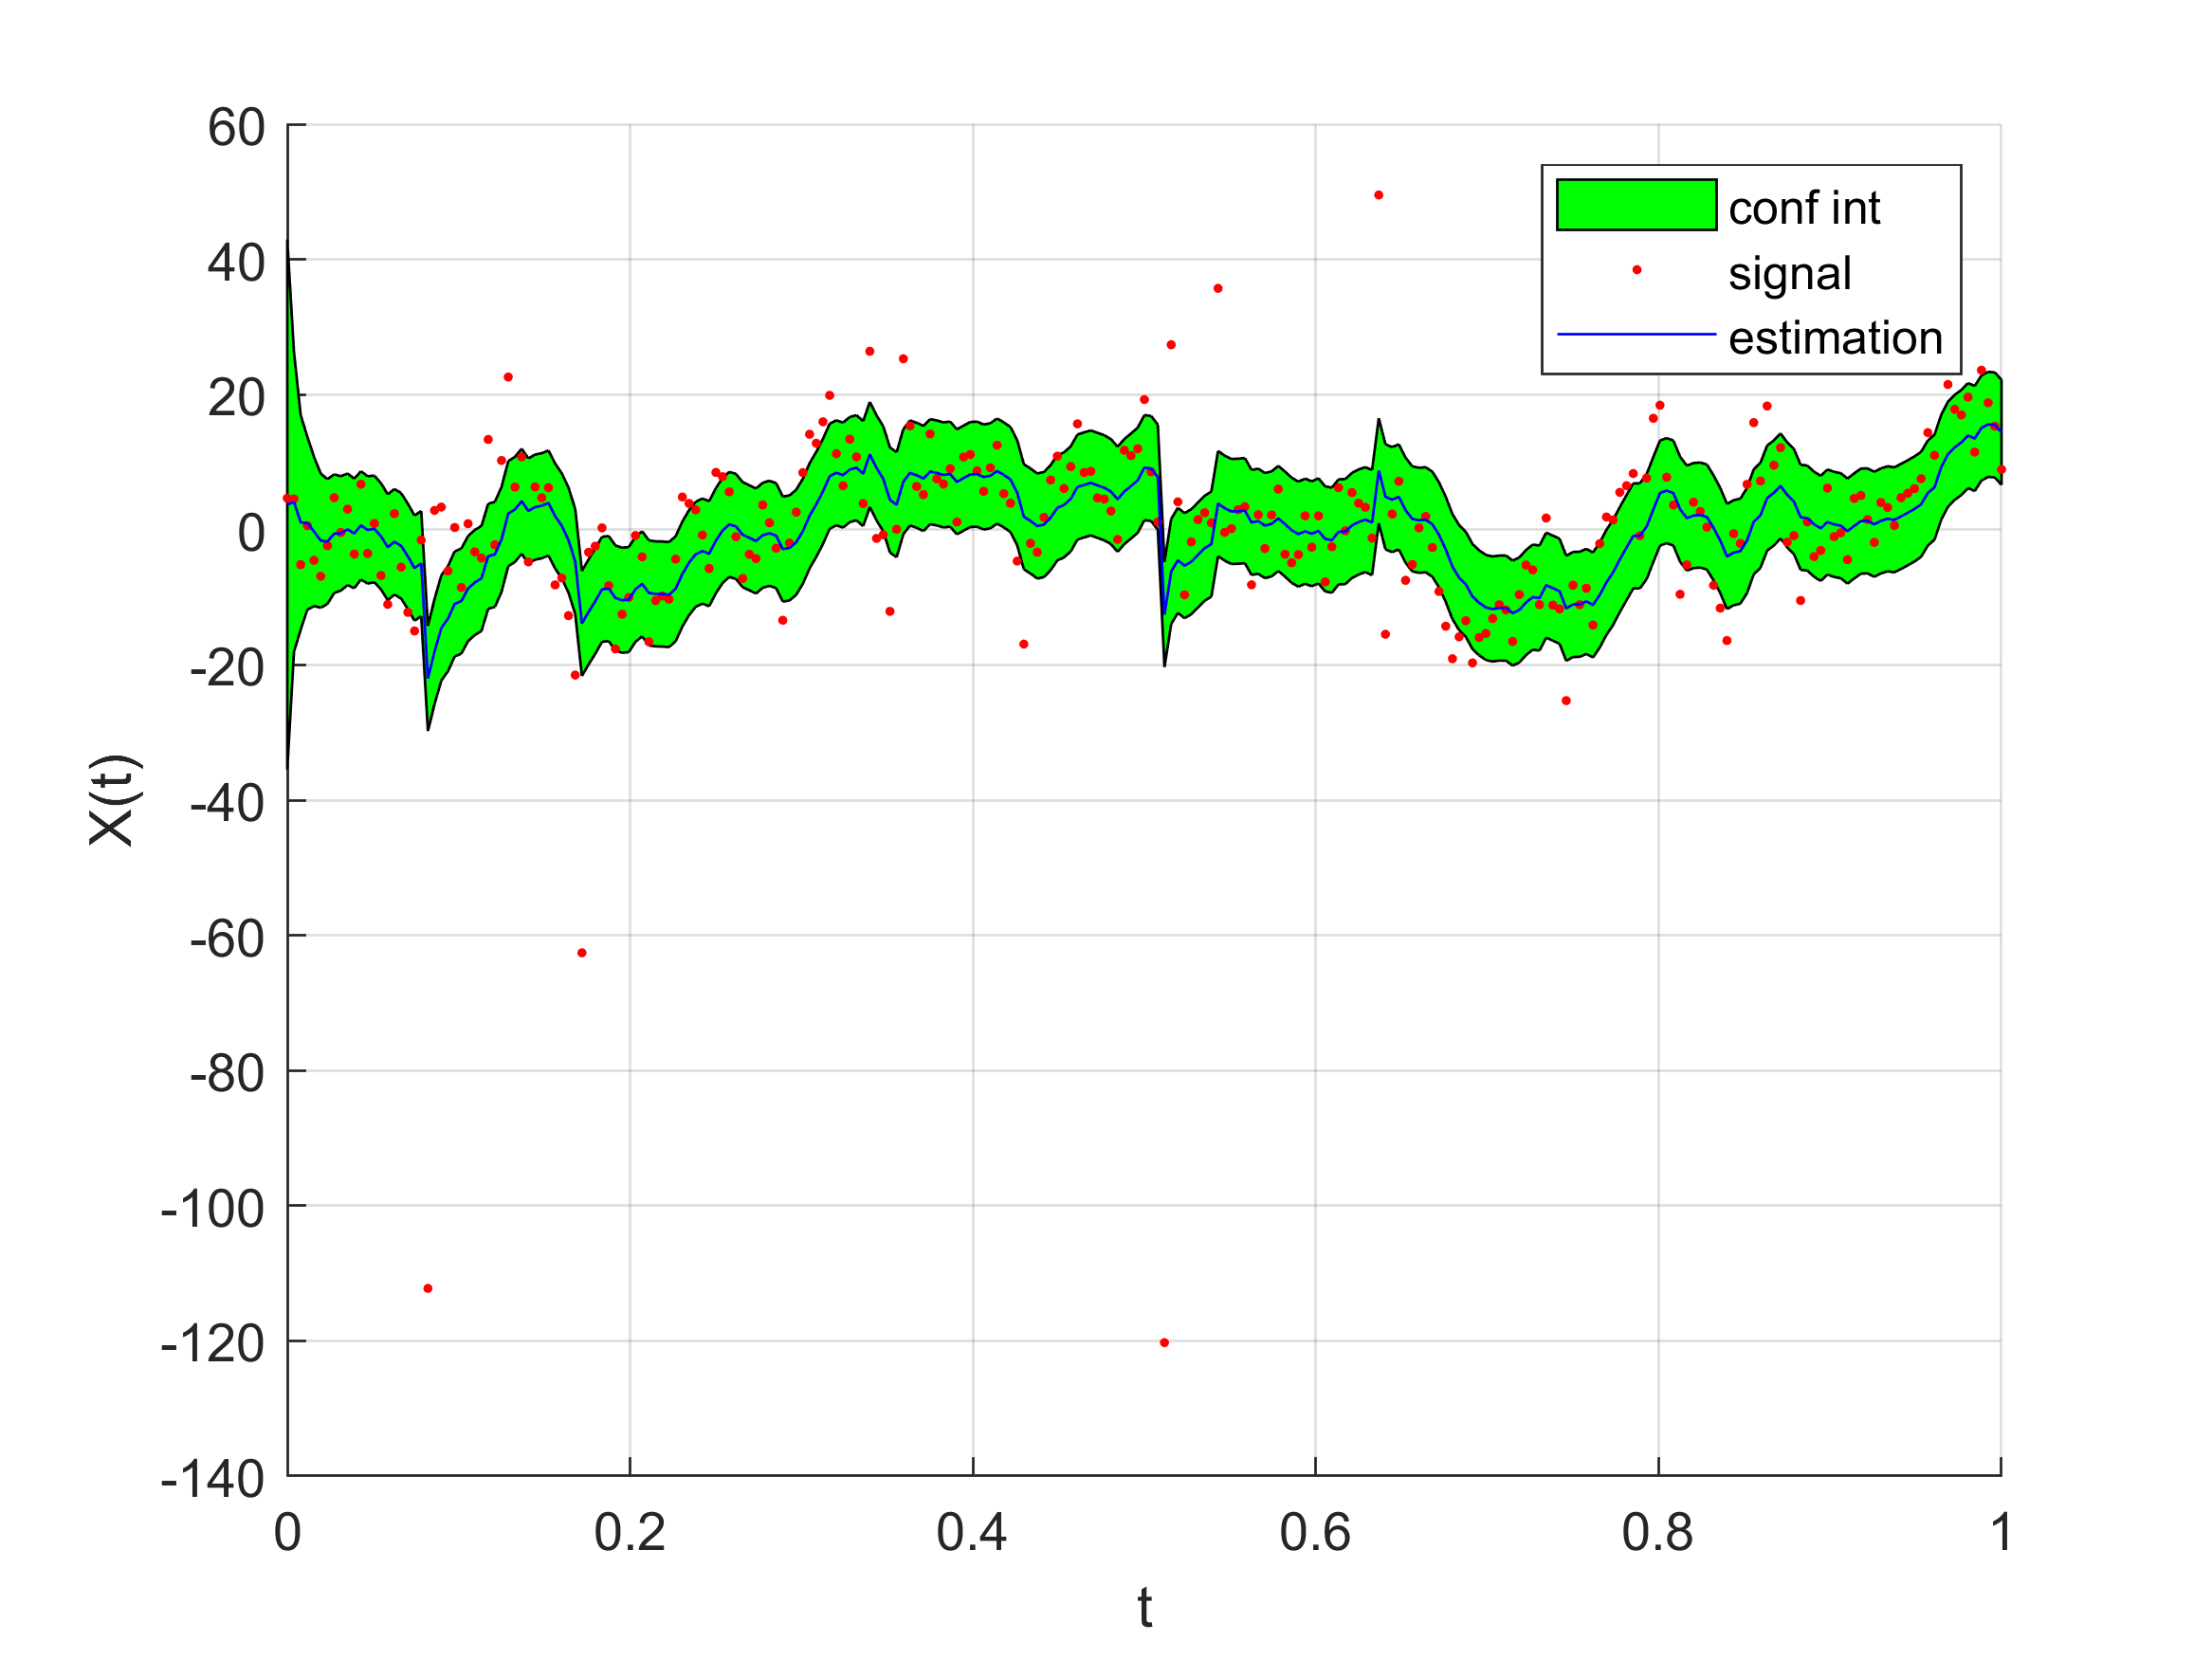
\includegraphics[width=0.6\textwidth]{../code/Task_10/pict/cauchy_10_5_5_ex.png}
						\caption{Процесс с параметрами $\lambda = 0.1,\sigma_1 = 5,  
										\sigma_2 = 10, T = 1$. Шум с $\gamma = 5$. }
				    \end{figure}
				    \begin{figure}[h!]
						\centering
						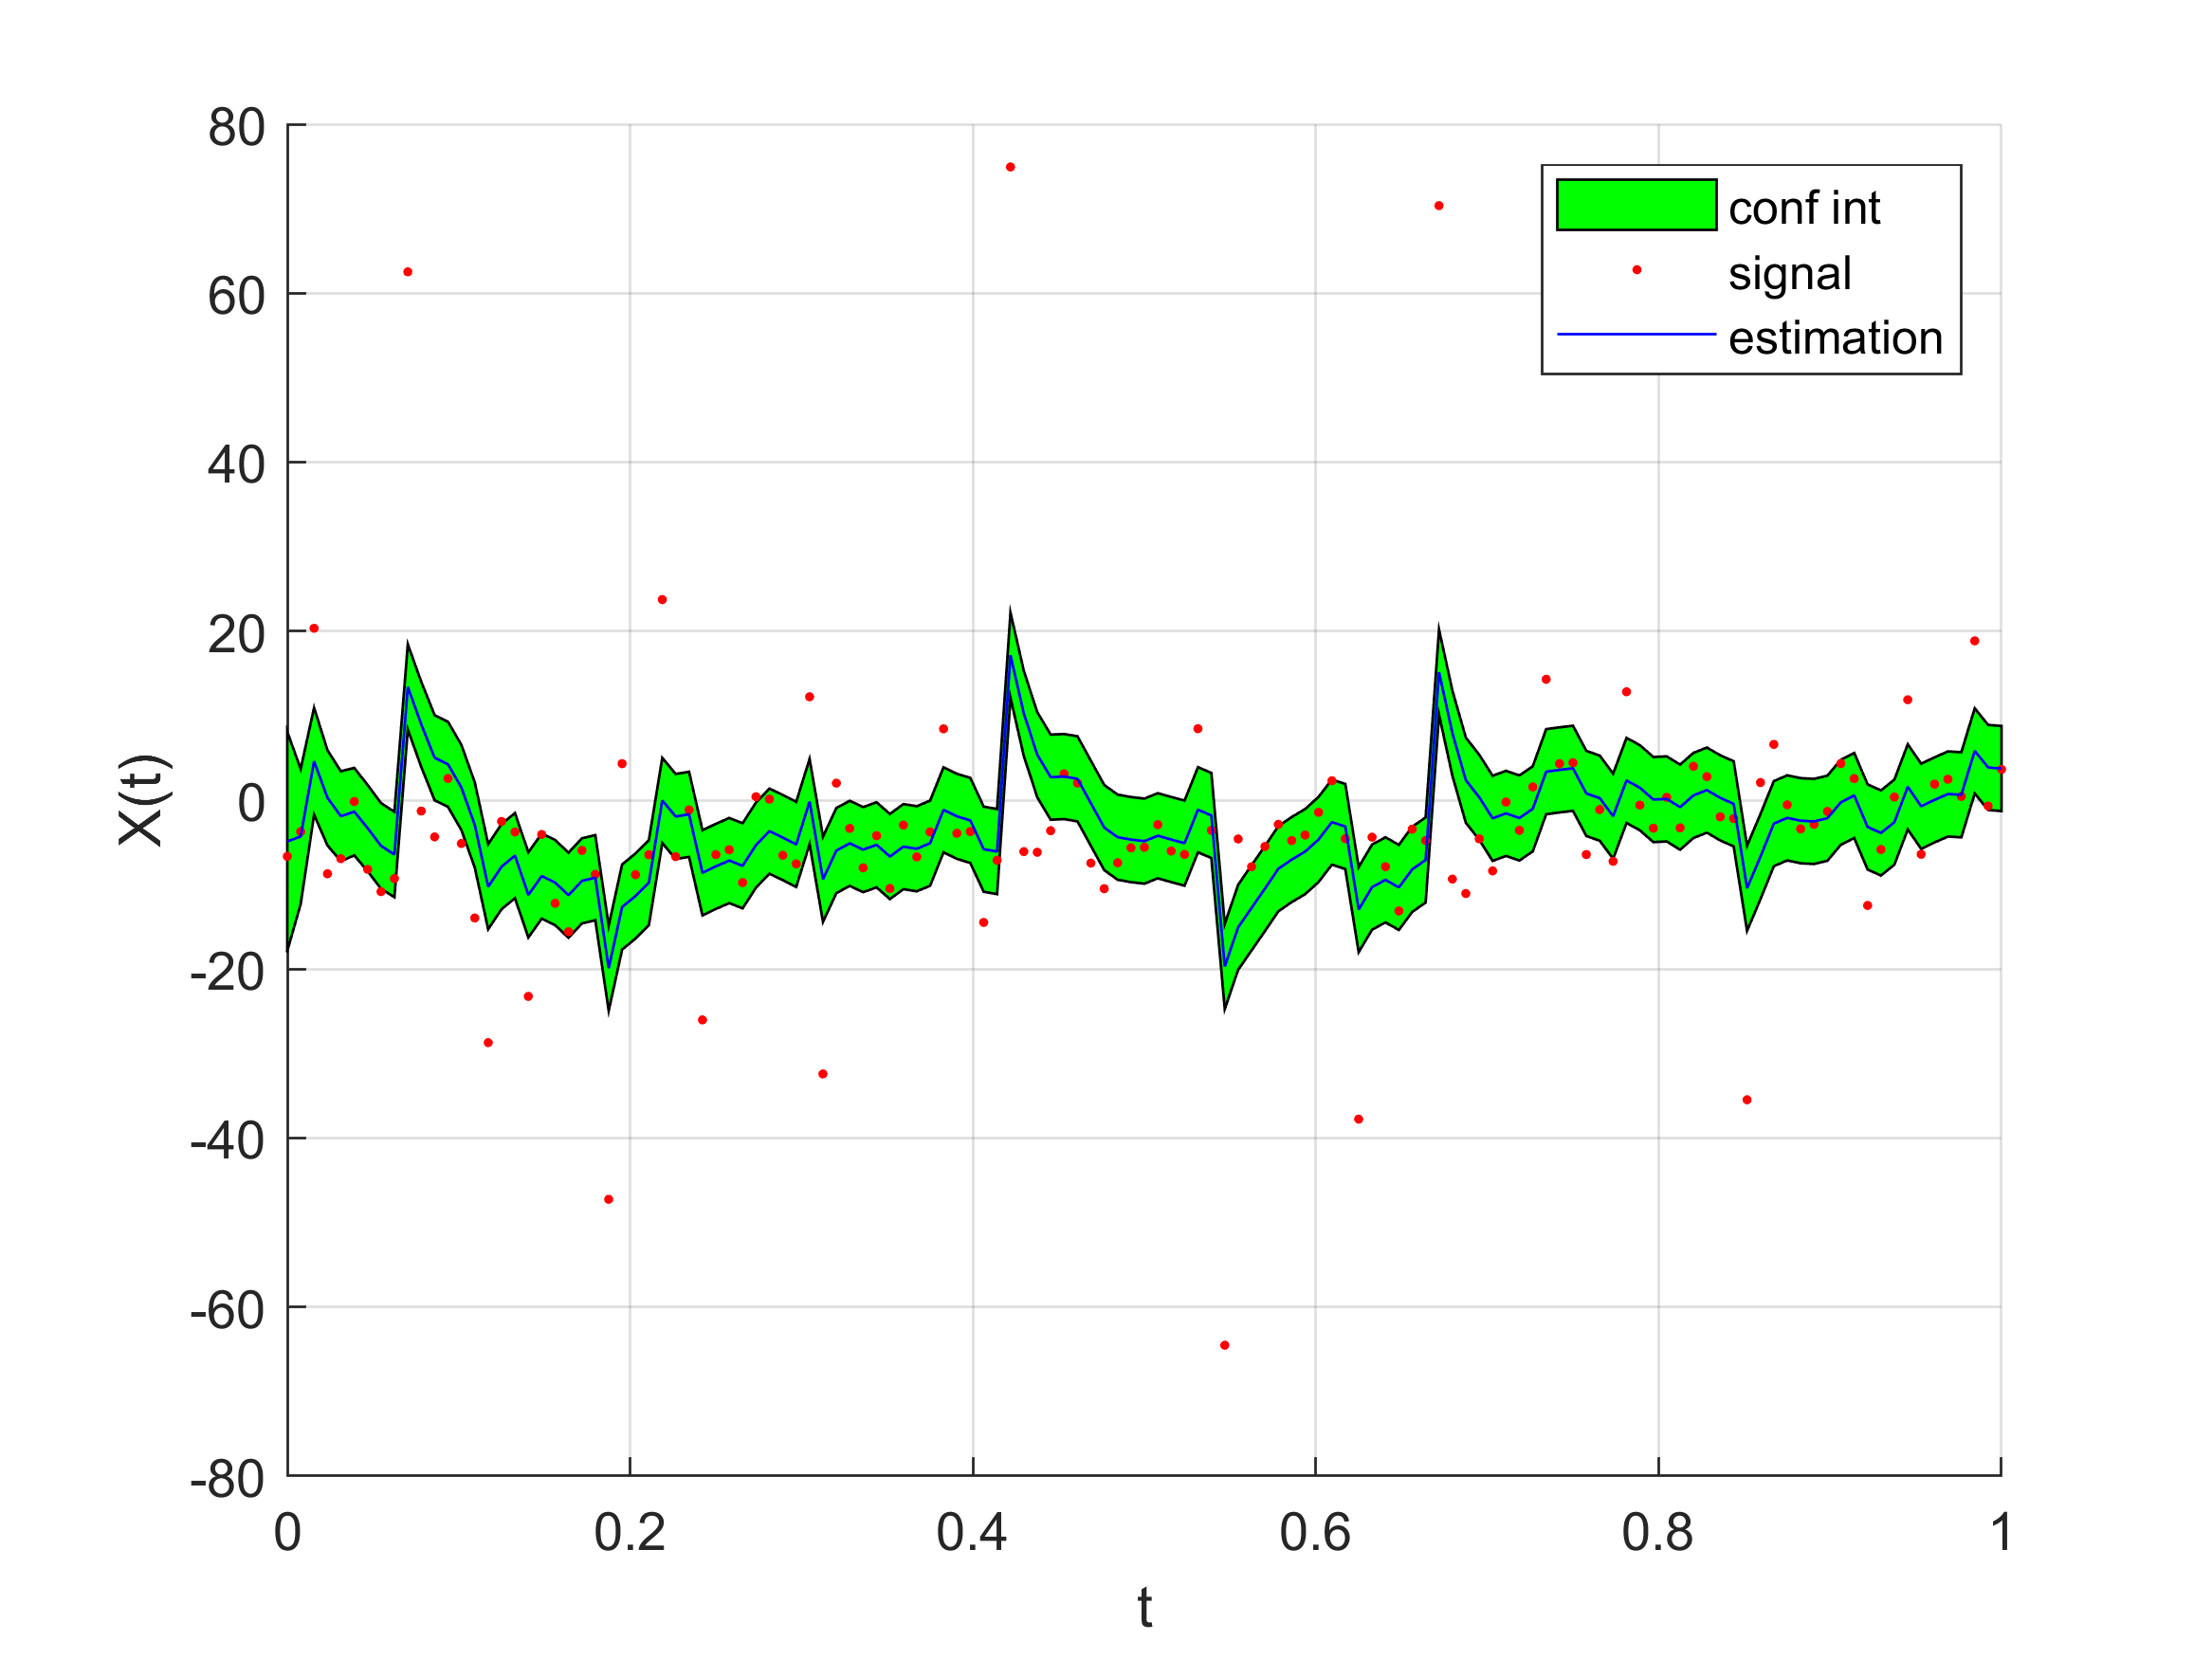
\includegraphics[width=0.6\textwidth]{../code/Task_10/pict/cauchy_5_10_3_ex.png}
						\caption{Процесс с параметрами $\lambda = 0.1,\sigma_1 = 5, \sigma_2 = 3, T = 1$. 
											Шум с $\gamma = 3$.}
				    \end{figure}
				    
		
				    Как мы видим, траектория процесса --- это либо почти весь зашумленный сигнал, либо
				   	траектория просто повторяет форму входного сигнала, фильтрация не работает. 
				   	Это происходит из-за того, что распределение Коши не имеет ни первых, 
				    ни вторых моментов, поэтому фильтр Калмана для таких шумов не применим.
	\end{itemize}
\newpage
\section{Задание 11}

\subsection{Постановка задачи}
    Построить двумерное пуассоновское поле, отвечающее сложному пуассоновскому процессу:
    \begin{enumerate} 
        \item Первая интерпретация: система массового обслуживания. При этом, первая координата поля ---
        		время поступления заявки в СМО (равномероное распределение), вторая --- время ее обслуживания
        		(распределение $\chi^2$ с 10 степенями свободы).
        \item Вторая интерпретация: система массового обслуживания с циклической интенсивностью 
        		$\lambda (1+\cos(t))$ и единичными скачками. Свести данную задачу моделирования
        		неоднородного пуассоновского процесса при помощи метода Льюиса и Шедлеара к моделированию 
        		двумерного пуассоновского поля, где первая координата имеет равномерное распределение, а 
        		вторая --- распределение Бернулли. 
        \item Третья интерпретация: работа страховой компании. Первая координата --- момент наступления 
        		страхового случая (равномерное распределение), вторая координата --- величина ущерба 
        		(распределение Парето). Поступления капитала по времени линейно со скоростью $c>0$, 
        		начальный капитал $W>0$.	
		\item Для каждой системы рассмтреть всевозможные случаи поведения системы в зависимости от
				значения параметров.
    \end{enumerate}
\subsection{Решение задачи}
\subsubsection{Пункт 1}
	Будем моделировать систему по следующему алгоритму:
	\begin{enumerate}
		\item Генерируем время поступления заявок на интервале $[0;T]$:
			$$ 0 \leqslant t_1\leqslant t_2 \leqslant \ldots \leqslant t_n \leqslant T, $$
			где $t_i - t_{i-1} \sim \exp(\lambda)$, $\lambda > 0$ -- интенстивность процесса Пуассона. 
		\item Генерируем время обработки заявок $s_i$ с помощью распределения $\chi^2$ с 10 степенями 
				свободы. 
		\item Для каждой заявки рассмотри время окончания ее выполнения $q_i$ 
			и количество заявок в очереди $n_i$:
				\begin{itemize}
					\item К моменту поступления заявки $t_i$ очереди нет, т.е. $q_{i-1}<t$. Тогда $q_i = t_i + s_i$, 
						и $n_i = 0$.
					\item К моменту поступления заявки $t_i$ какая-то заявка исполняется, 
						т.е. $q_{i-1}\geqslant t_i$. Пусть выполнено только $n_{fin}$ заявок к предыдущему 
						моменту $t_{i-1}$.
						Тогда мы пересчитываем $n_{fin}$ для данного момента (т.е. находим
						самую позднюю заявку $fin$ для которой $q_{fin} \leqslant t_i$)
						и кладем $n_i = i - n_{fin}$, $q_i = q_{i-1}+ s_i$.
				\end{itemize}
				В среднем, время обслуживания составляет, $$\E  s_i = 10, $$
				а среднее время поступления новой заявки равно: $$\E  (t_i - t_{i-1}) =\frac{1}{\lambda}.$$
				Тогда при $\lambda < 0.1$ система будет справляться, при $\lambda > 0.1$ очередь будет 
				неограниченно расти. При $\lambda = 0.1$ будет некоторое промежуточное состояние.
	\end{enumerate}
	\begin{figure}[h!]
		\centering
		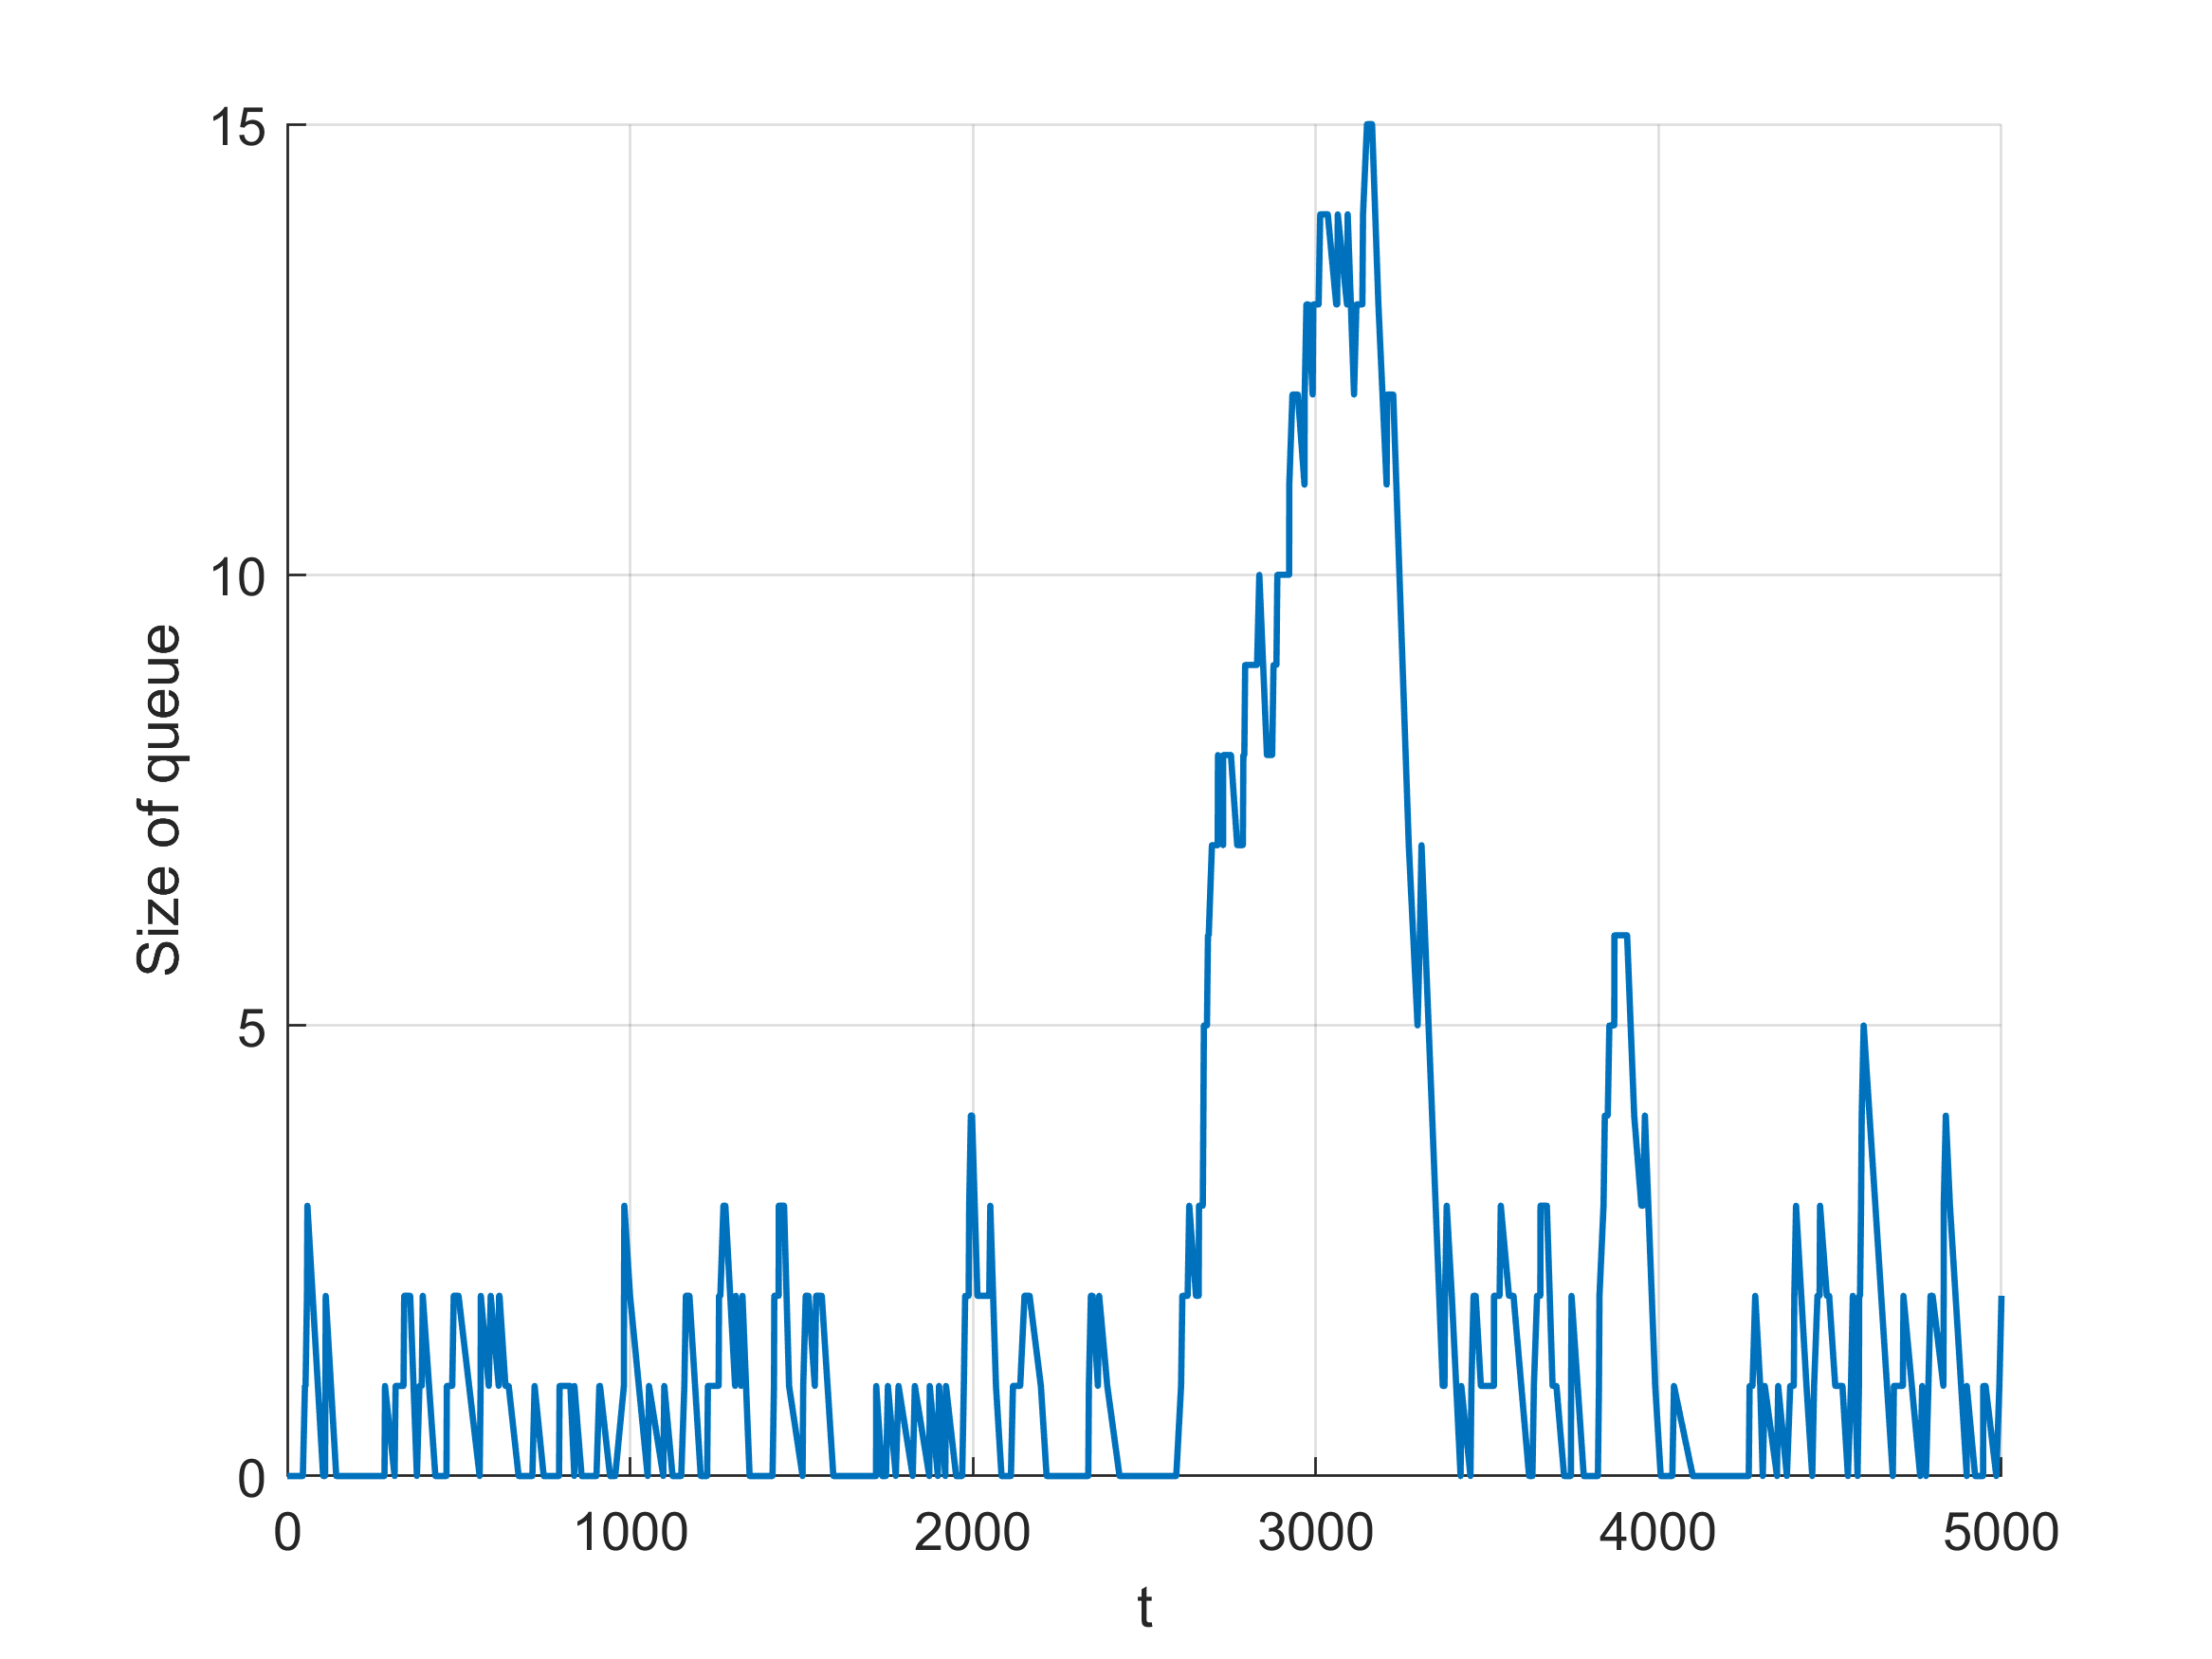
\includegraphics[width=0.6\textwidth]{../code/Task_11/pict/hom_7_ex.png}
		\caption{СМО справляется с очередью, $\lambda =  0.07$.}
    \end{figure}
    \begin{figure}[h!]
		\centering
		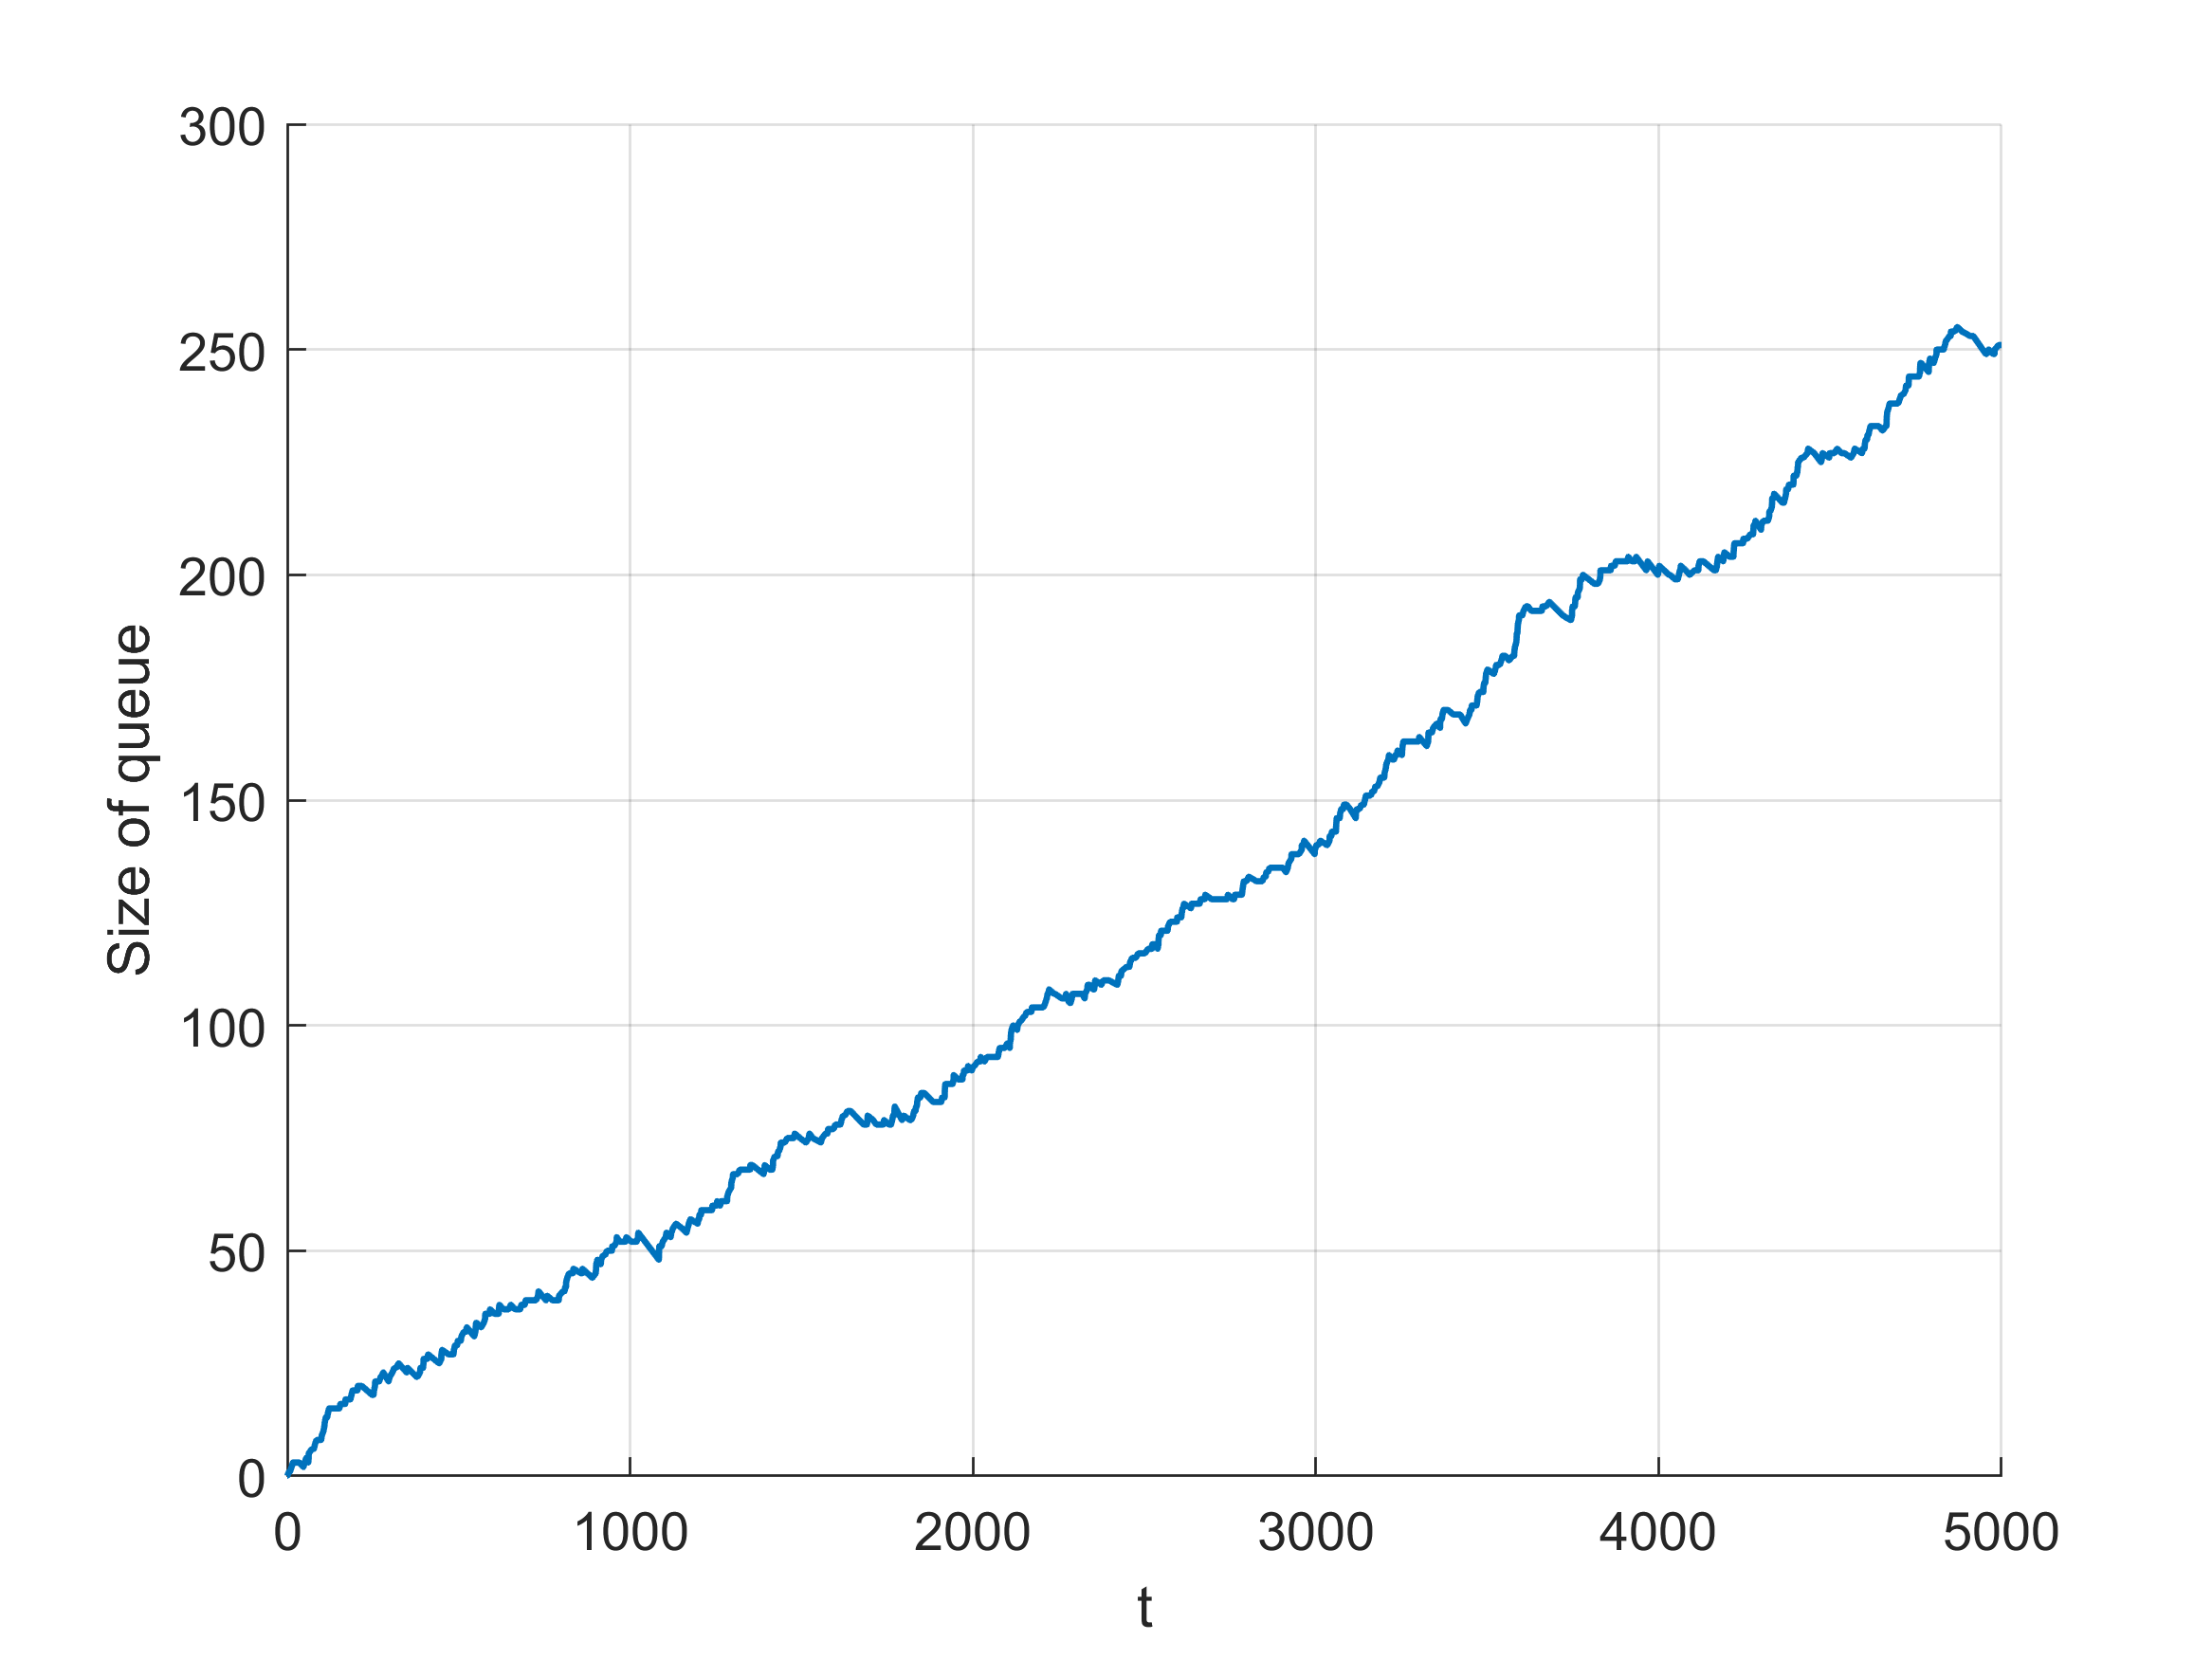
\includegraphics[width=0.6\textwidth]{../code/Task_11/pict/hom_15_ex.png}
		\caption{СМО не справляется с очередью, $\lambda =  0.15$.}
    \end{figure}
    \begin{figure}[h!]
		\centering
		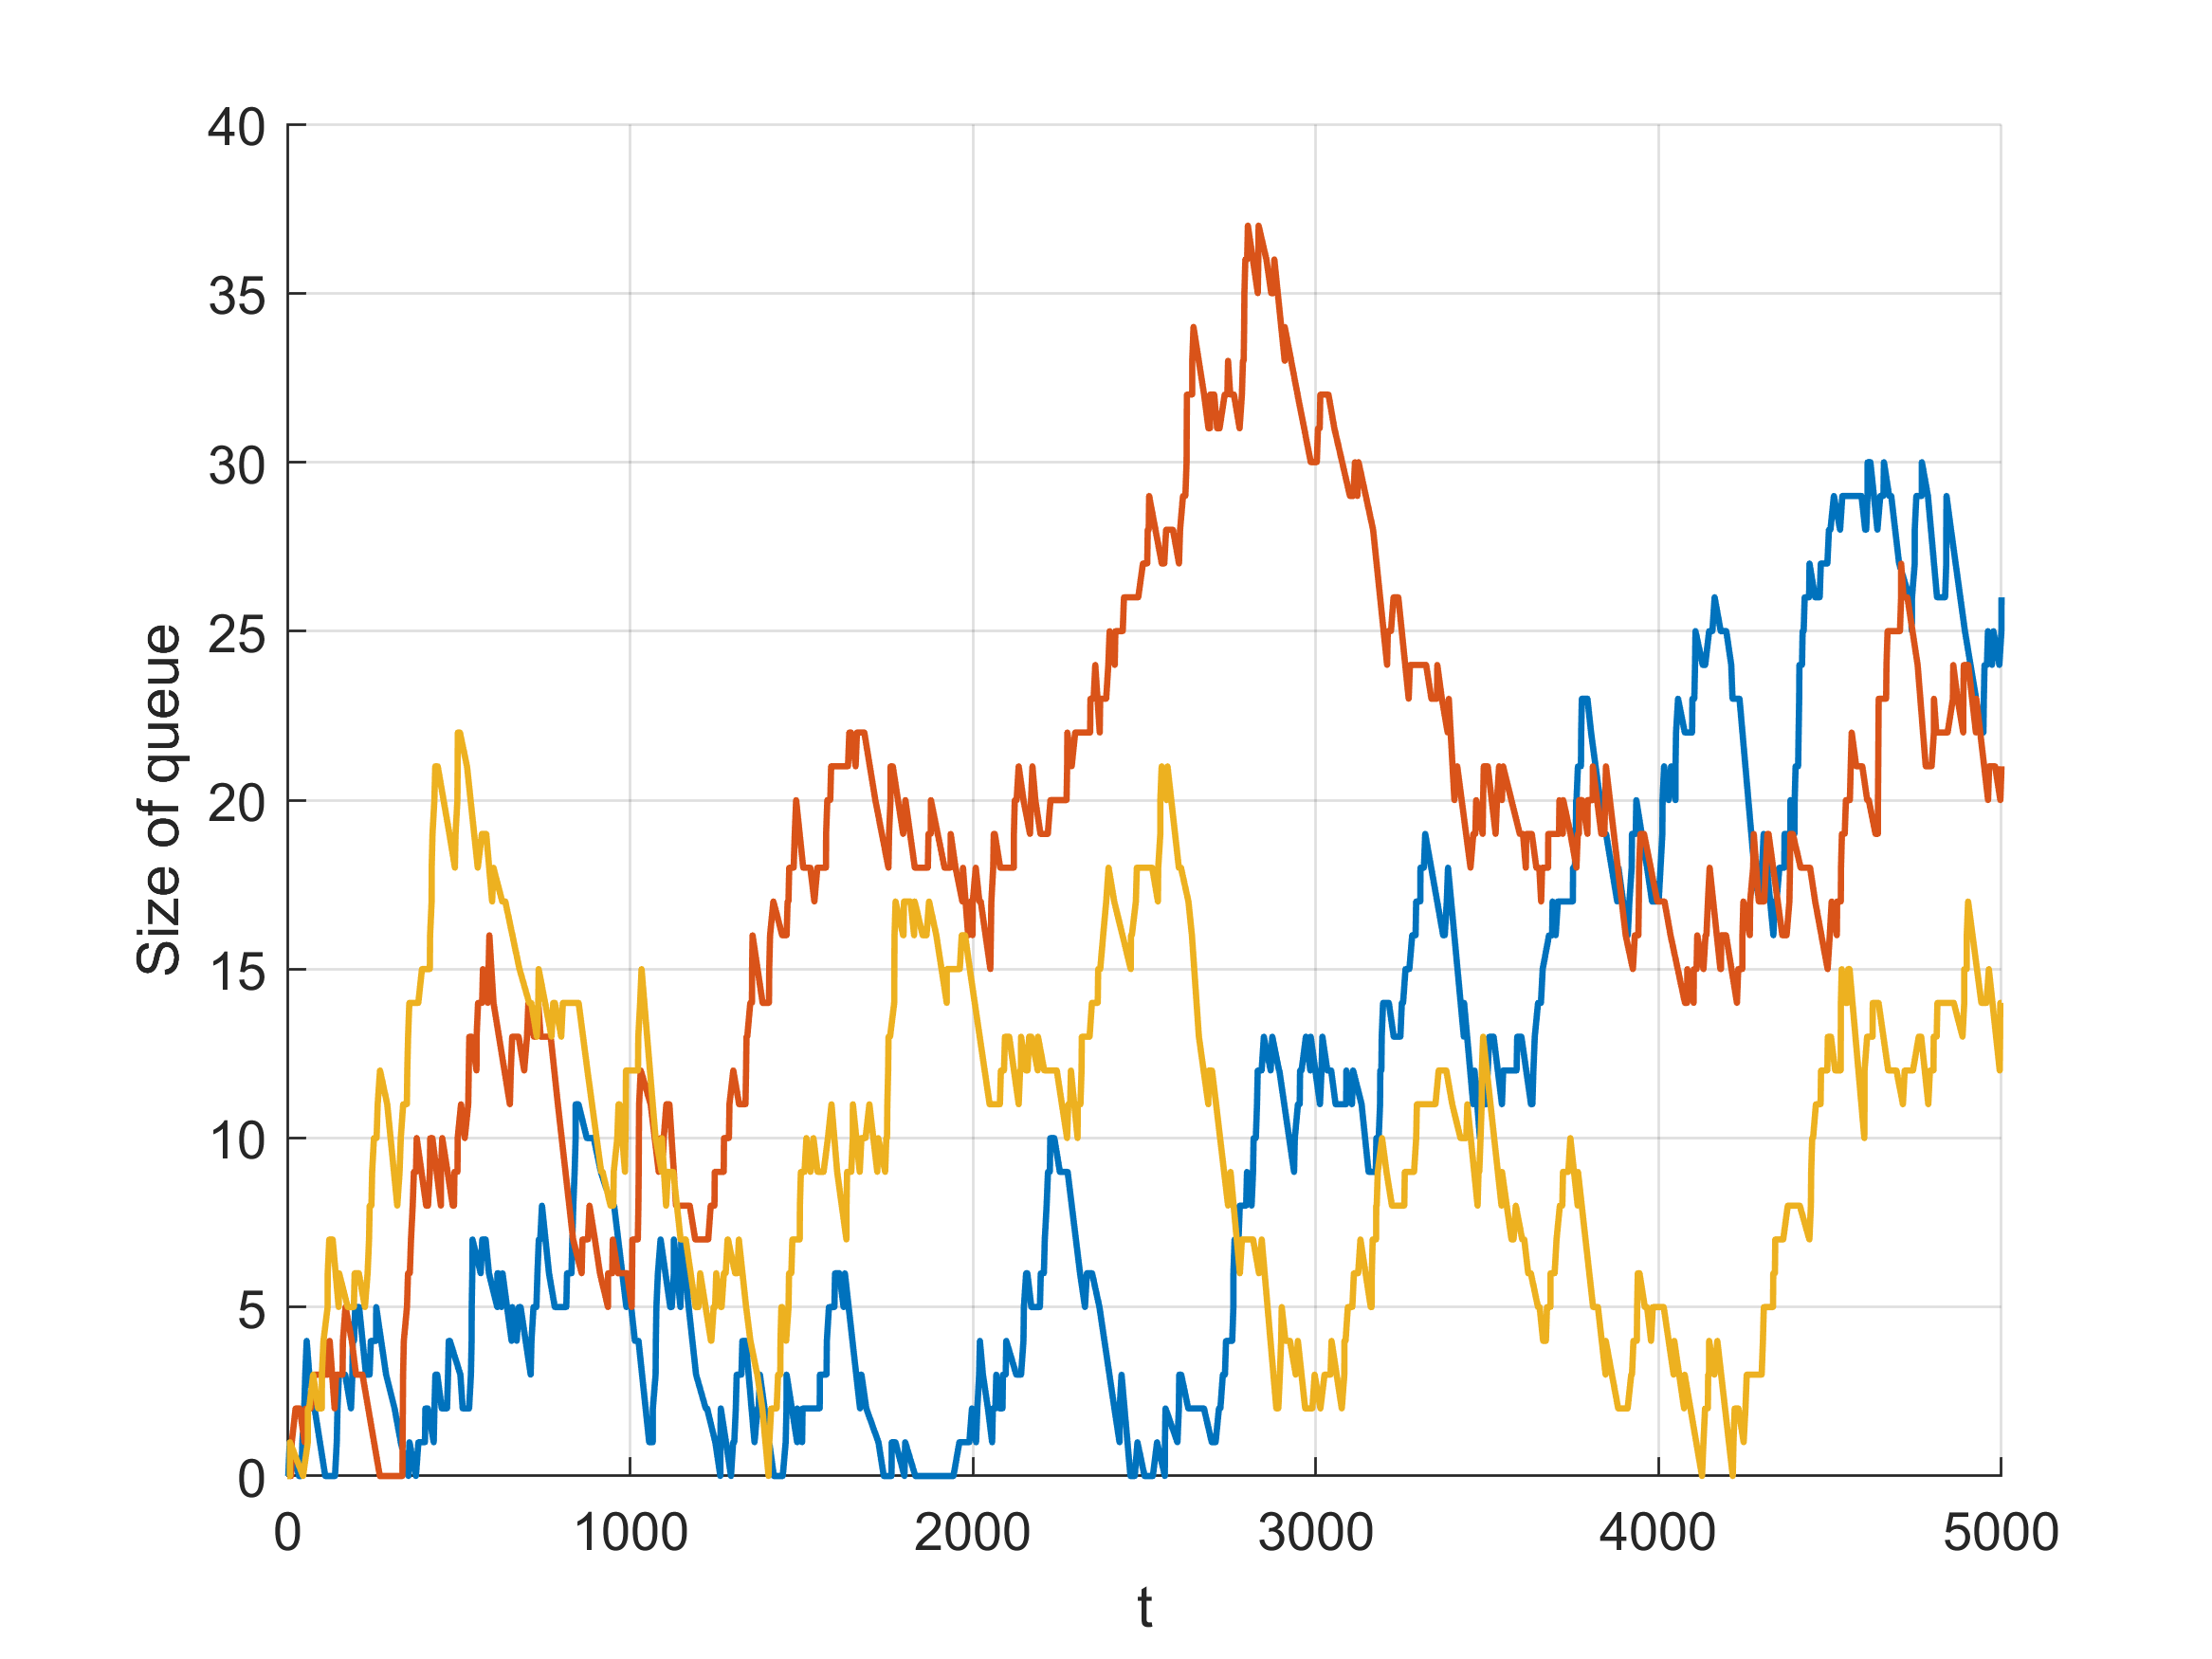
\includegraphics[width=0.6\textwidth]{../code/Task_11/pict/hom_10_ex.png}
		\caption{СМО в промежуточном состоянии, $\lambda =  0.1$.}
    \end{figure}

\newpage    
\subsubsection{Пункт 2}

	Теперь рассмотрим СМО с циклической интенсивностью $\lambda(t) = \lambda_0 (1+\cos(t))$. Интегральная 
	интенсивность $\Lambda(t) = \int\limits_0^t \lambda(x)dx = \lambda_0 (1+\sin(t))$.
	\begin{theorem}
		Рассмотрим одномерный неоднородный процесс Пуассона $[N^*(x): x\geqslant 0]$ с интенсивностью
		$\lambda^*(x)$ такой, что число точек $N^*(x_0)$ на фиксированном интервале $(0;x_0]$ имеет 
		распределение Пуассона с параметром $\mu^*_0 = \Lambda^*(x_0)-\Lambda^*(0)$. 
		Положим $X^*_1, X^*_2,\ldots X^*_{N^*(x_0)}$ точками данного процесса на $(0;x_0]$. 
		Предположим, что при $0 \leqslant x \leqslant x_0$, $\lambda(x) \leqslant \lambda^*(x)$. 
		Для каждого $i = 1,2,\ldots, n,$ удаляем точку $X^*_i$ с вероятностью
		$1-\lambda(x^*_i) \slash \lambda^*(x^*_i)$. 
		После этого оставшиеся точки будут образовывать неоднородный процесс Пуассона
		$[N(x): x\geqslant 0]$ с интенсивностью $\lambda(x)$  на интервале $(0;x_0]$.
	\end{theorem}
	Доказательство этой теоремы приведено в $\cite{article}$.
	
	\vspace{5mm}\noindent 
	В соответствии с теоремой будем моделировать наш процесс по следующему алгоритму:
	\begin{itemize}
		\item Генерируем времена поступления заявок процесса $N^*(t): X^*_1, X^*_2,\ldots X^*_n$ 
			c частотой $\lambda^*(x) = 2$ (см. 5.2.1).
		\item Генерируем вектор $U$ из $n$ независимых с.в. с равномерным распределением на $[0;1]$. 
			Формируем вектор времен поступления заявок процесса $N(t)$, из тех $X^*_i$, 
			для которых  $U_i \leqslant \lambda(x^*_i) \slash \lambda^*(x^*_i)$, не меняя их порядка. 
	\end{itemize}
	
	\begin{figure}[h!]
		\centering
		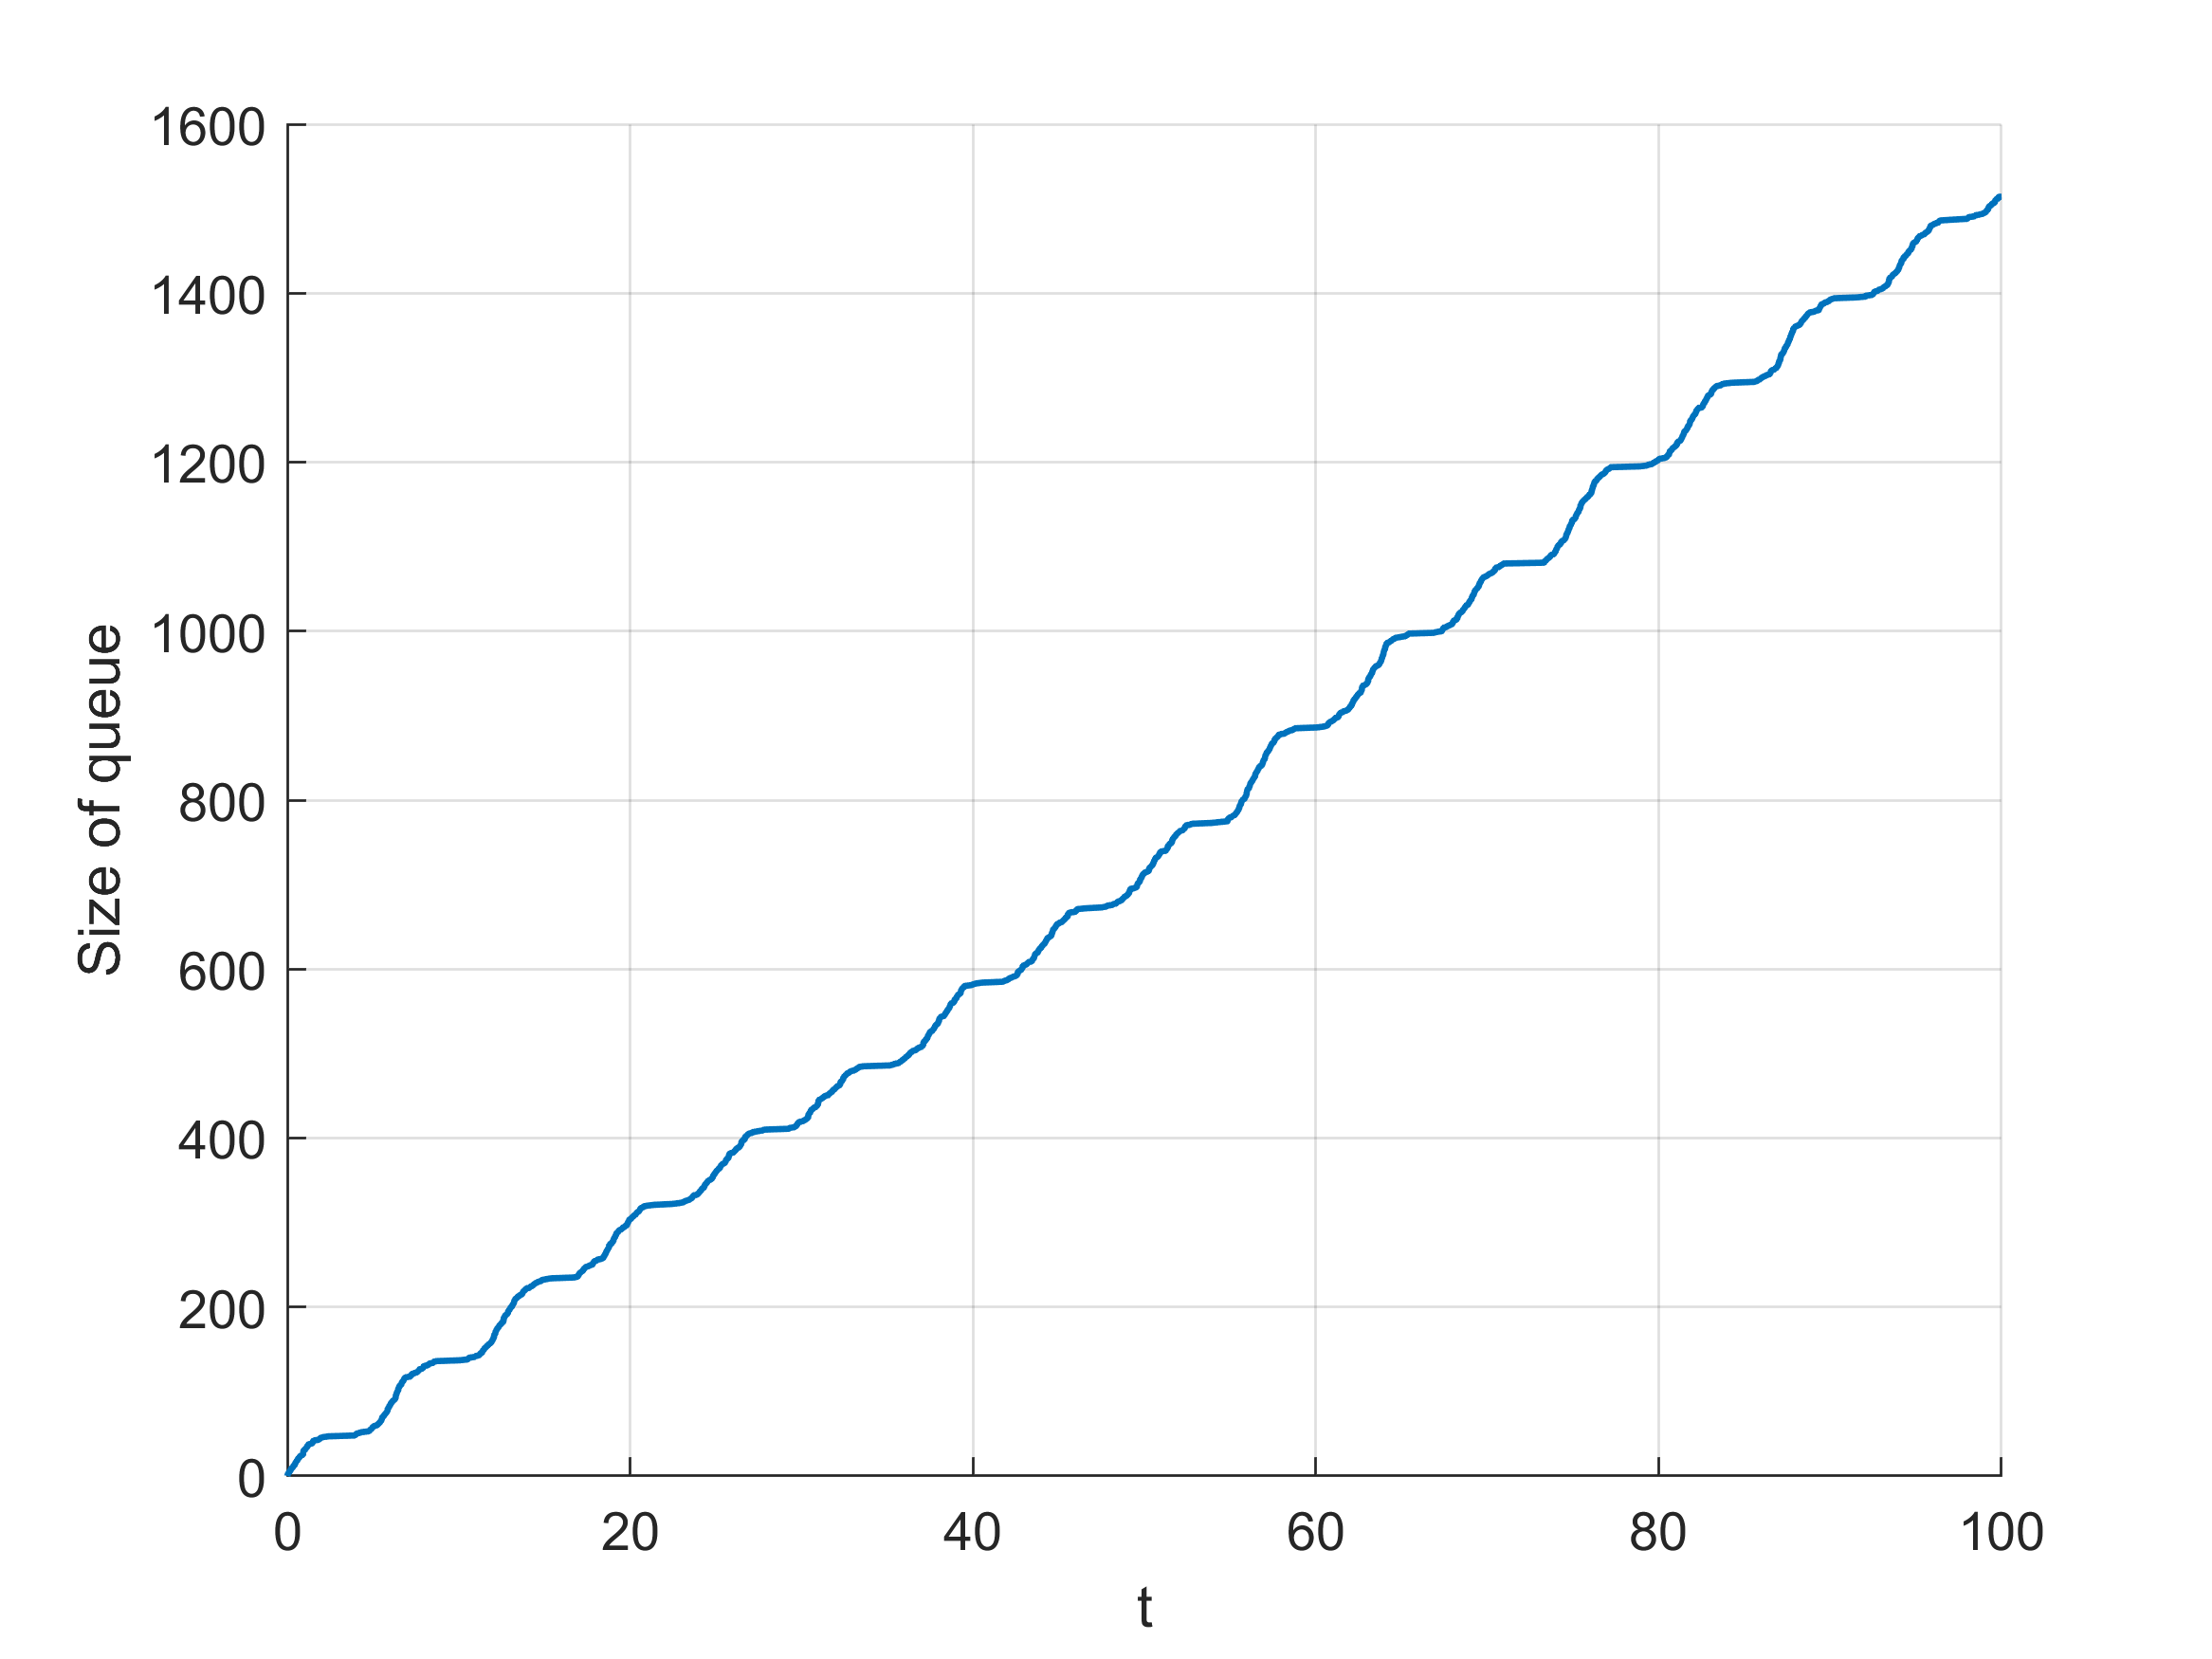
\includegraphics[width=0.6\textwidth]{../code/Task_11/pict/nonhom_1500_ex.png}
		\caption{СМО c циклической частотой при $\lambda_0 =  15$.}
    \end{figure}
    
\newpage
\subsubsection{Пункт 3}
	
	\begin{definition}
		Случайная величина $\xi$ называется случайной величиной, имеющей распределение Парето
		 с параметрами $x_m, k$, если ее функция распределения имеет вид:
		 $$ F_X(x) = \mathbb{P}(X<x) = 1- \left( \frac{x_m}{x}\right)^k 
		 \quad \forall x\geqslant x_m, \quad x_m, k> 0.$$
	\end{definition}
	\noindent
	Аналогично пункту 1 задачи, генерируем вектор поступления страховых случаев на $[0;T]$.
	\newline
	Величину ущерба $s_i$ будем генерировать с помощью распределения Парето с параметрами $x_m, k$.
	
	Случайную величину, распределенную по Парето, будем генерировать методом обратных функций:
	\begin{equation}
		F^{-1}(y) = \frac{x_m}{{(1-y)}^{\frac{1}{k}}}. \label{inv_func}
	\end{equation}
	Как отмечалось ранее, если $Y\sim U[0;1]$, то с.в., полученная по правилу ($\ref{inv_func}$), будет
	иметь ту же функцию распределения, что мы обратили:
	$$ Y \sim U[0,1] \Rightarrow s_i = x_m Y^{-\frac{1}{k}} \sim P(x_m,k).$$
	Величина капитала компании в момент времени $t$:
	$$W(t) = W_0 + ct - s(t),$$
	где $s(t) = \sum\limits_{i} s_i \mathbb{I}(t_i\leqslant t)$ --- суммарный ущерб 
	от наступивших страховых случаев.
	\newline Заметим, что  $s_i$ и $t_i$ являются независимыми случаными величинами и 
		$\E \sum\limits_{i}\mathbb{I}(t_i\leqslant t) = t \slash \lambda $.
	\newpage \noindent
	Проанализируем динамику $\E  W(t)$ c течением времени: 
	$$(\E  W(t))^{\prime}= c - (\E  s(t))^{\prime} = c 
			- \E  s_i \left(\E  \sum\limits_{i}\mathbb{I}(t_i\leqslant t) \right)^{\prime}=
			 c - \frac{1}{\lambda}\E  s_i, $$
	$$ 
		\E  s_i = \left \{
										\begin{aligned}
											&\dfrac{k x_m}{k-1}, \quad & k>1 \\
											& +\infty, & k \leqslant 1.
										\end{aligned}
									\right.
	$$
	\noindent
	Итого:
	$$ 
		(\E  W(t))' = \left \{
										\begin{aligned}
											& c - \dfrac{1}{\lambda}\dfrac{k x_m}{k-1}, \quad & k>1 \\
											& -\infty, & k \leqslant 1.
										\end{aligned}
									\right.
	$$
	Время разорения--- это случайная величина, задаваемая условием:
	$$ T = \min\{t>0| W(t)<0\}$$
	Это значит, что: 
	\begin{itemize}
		\item при c > $\dfrac{1}{\lambda}\dfrac{k x_m}{k-1}$ капитал будет возрастать:
			\begin{figure}[h!]
				\centering
				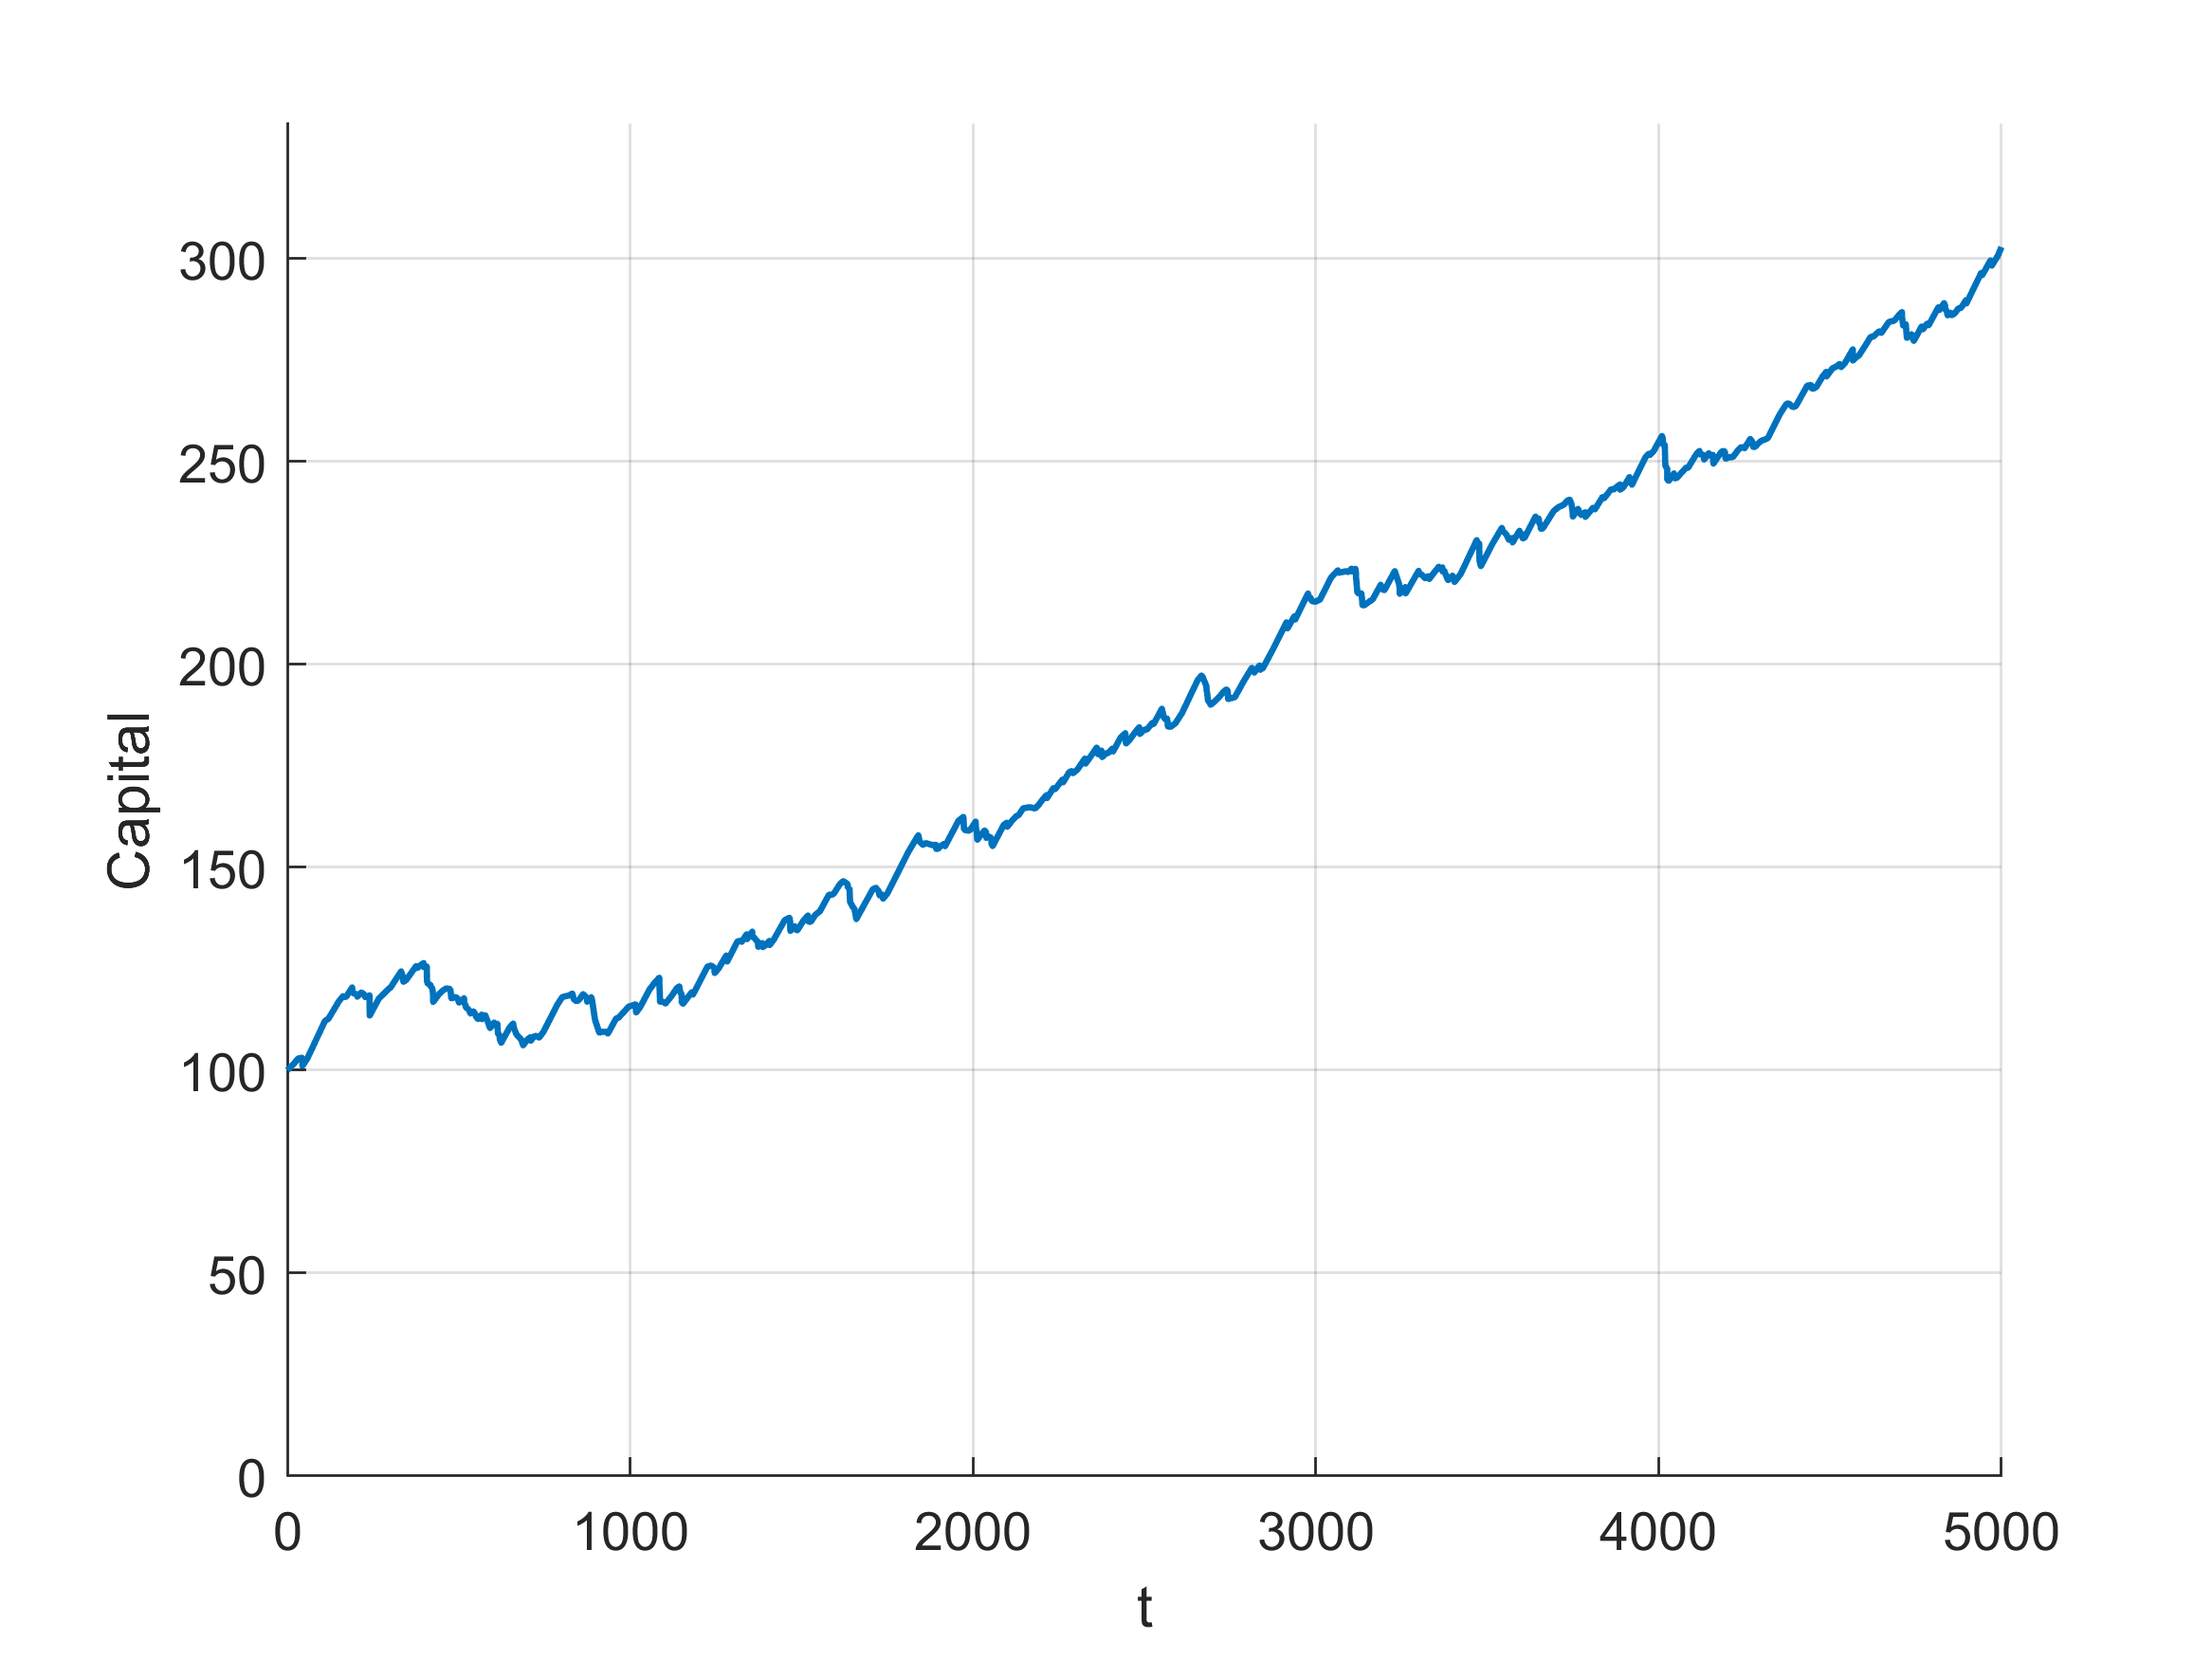
\includegraphics[width=0.6\textwidth]{../code/Task_11/pict/ins_10_100_20_3_ex.png}
				\caption{Капитал при $W_0 = 100, \lambda=  0.1, k=3, x_m =1, c =0.2, T=5000 $.}
		    \end{figure}
		\item при c < $\dfrac{1}{\lambda}\dfrac{k x_m}{k-1}$ капитал будет убывать, и компания в какой-то 
			момент разорится:
			\begin{figure}[h!]
				\centering
				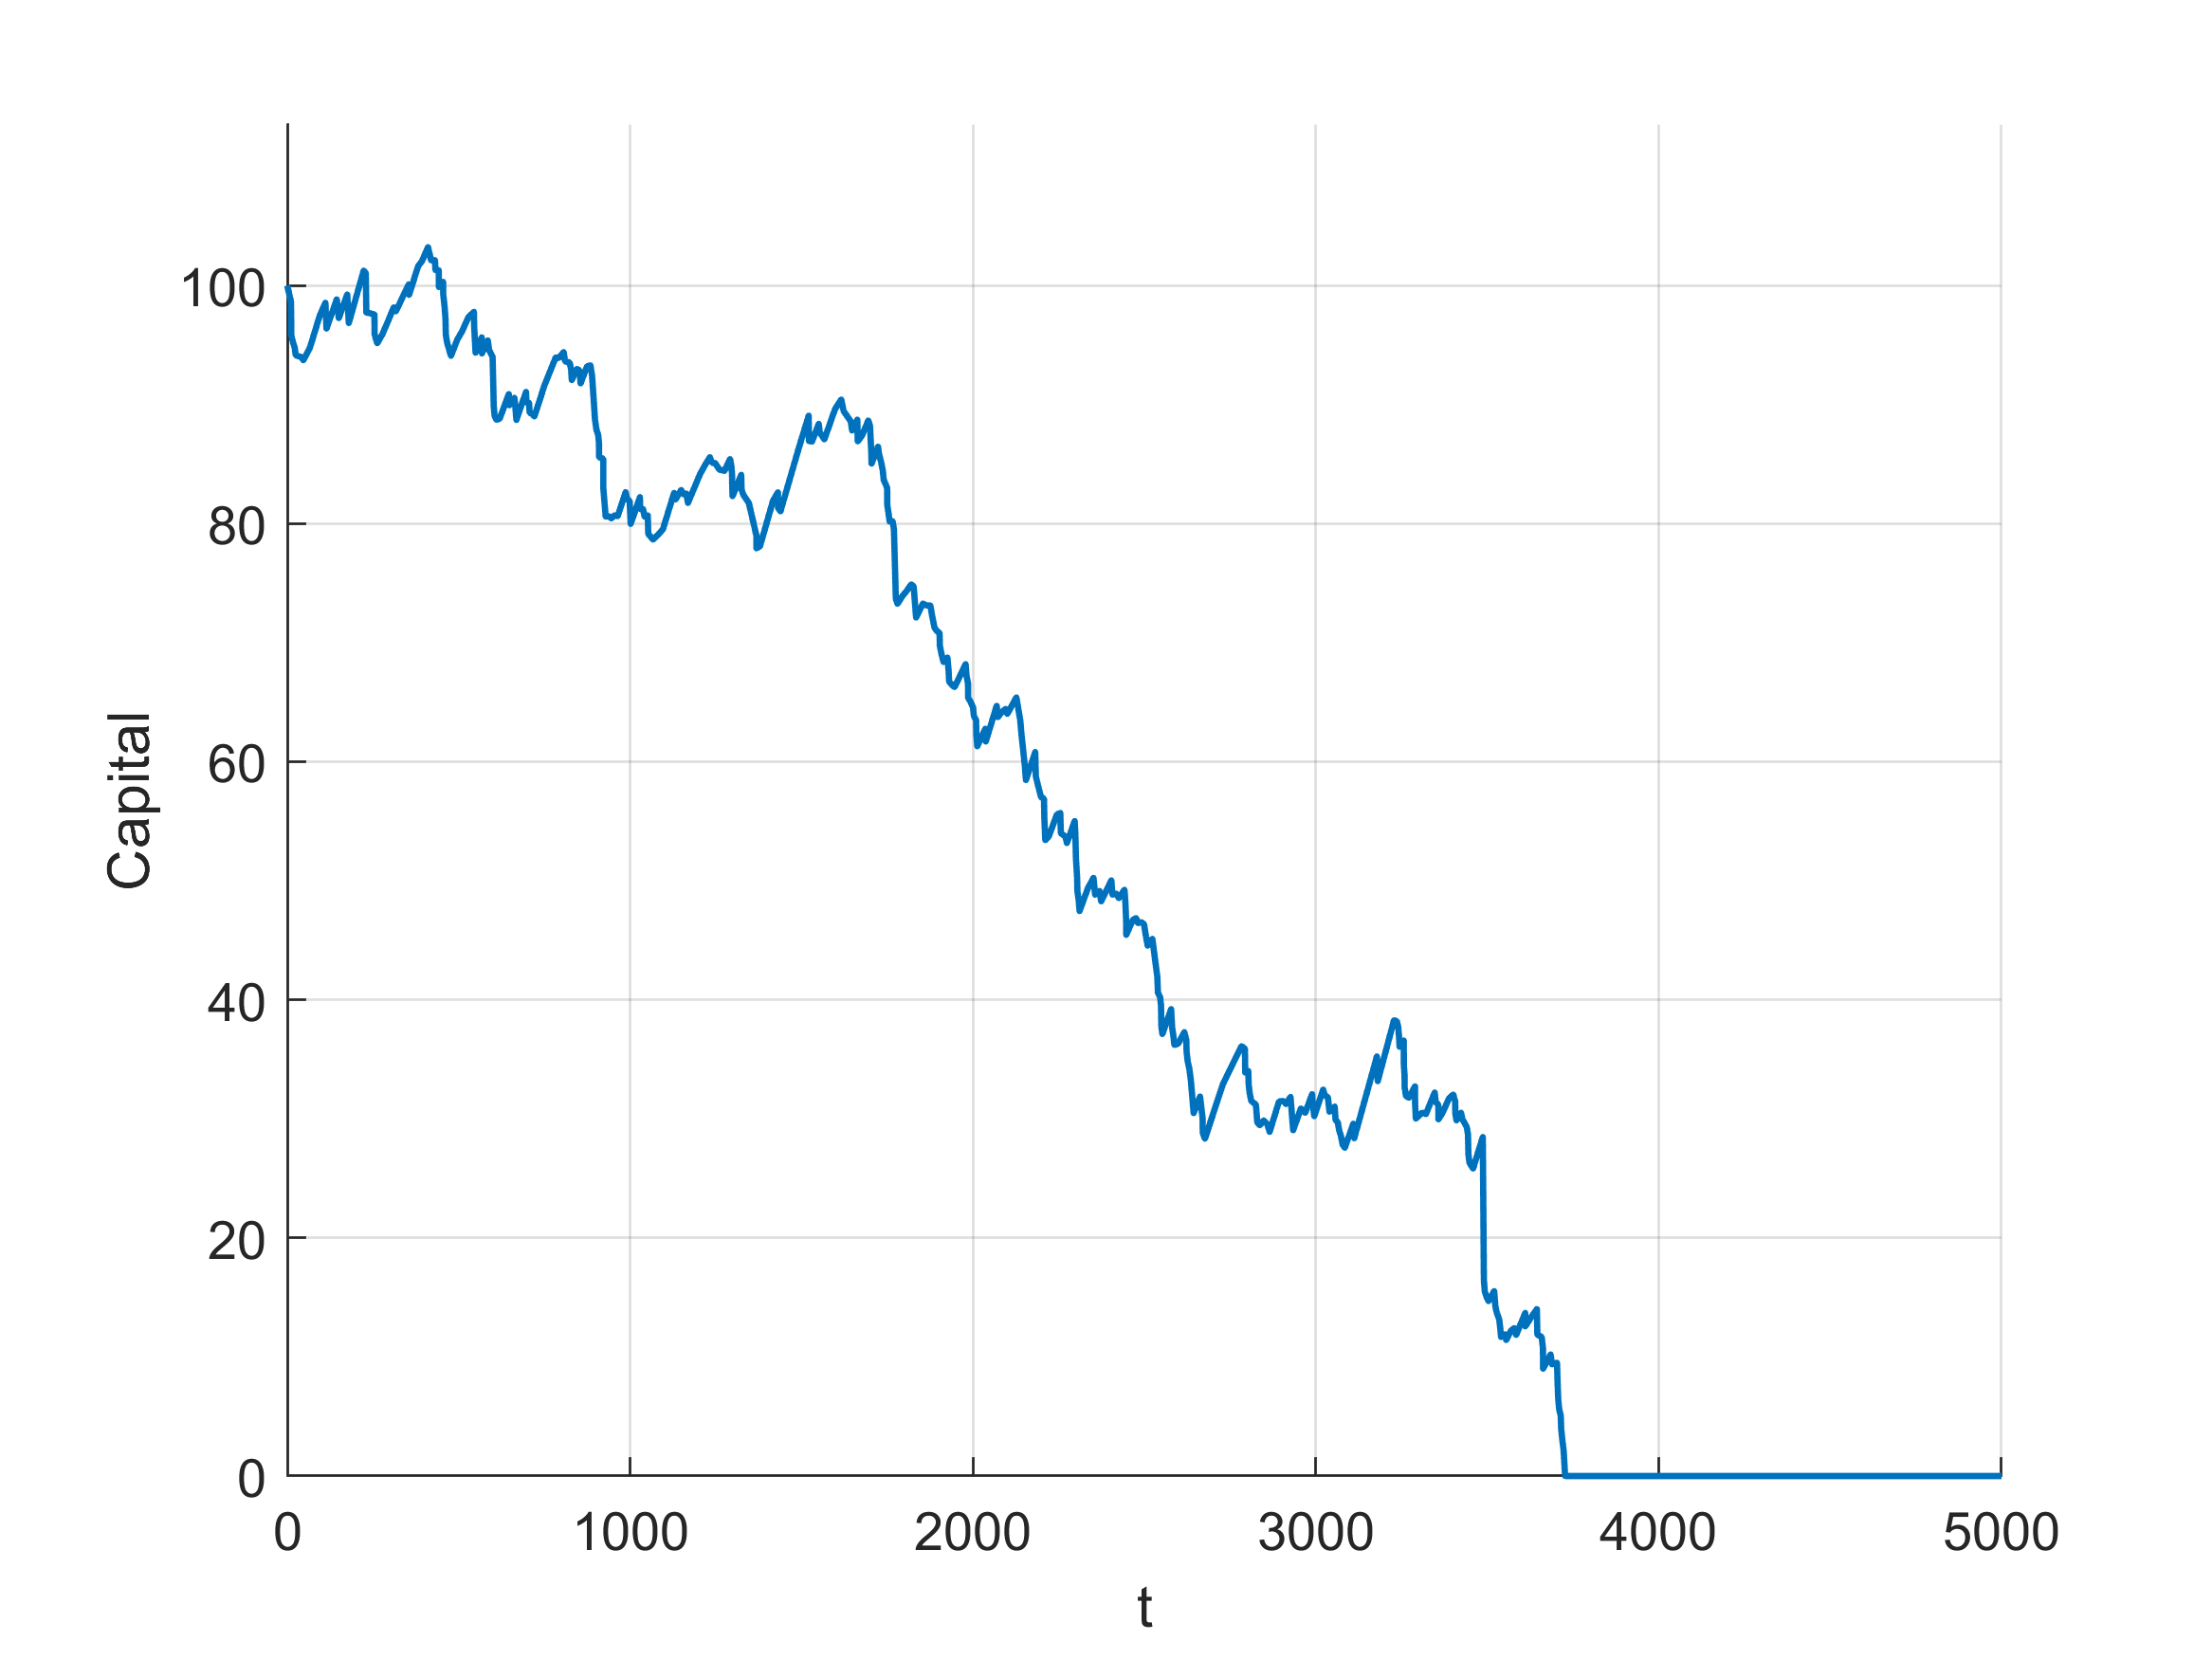
\includegraphics[width=0.6\textwidth]{../code/Task_11/pict/ins_10_100_13_3_ex.png}
				\caption{Капитал при $W_0 = 100, \lambda=  0.1, k=3, x_m =1, c =0.13, T=5000 $.}
		    \end{figure}
		\newpage
		\item при c = $\dfrac{1}{\lambda}\dfrac{k x_m}{k-1}$ капитал будет находится в положении равновесия:
			\begin{figure}[h!]
				\centering
				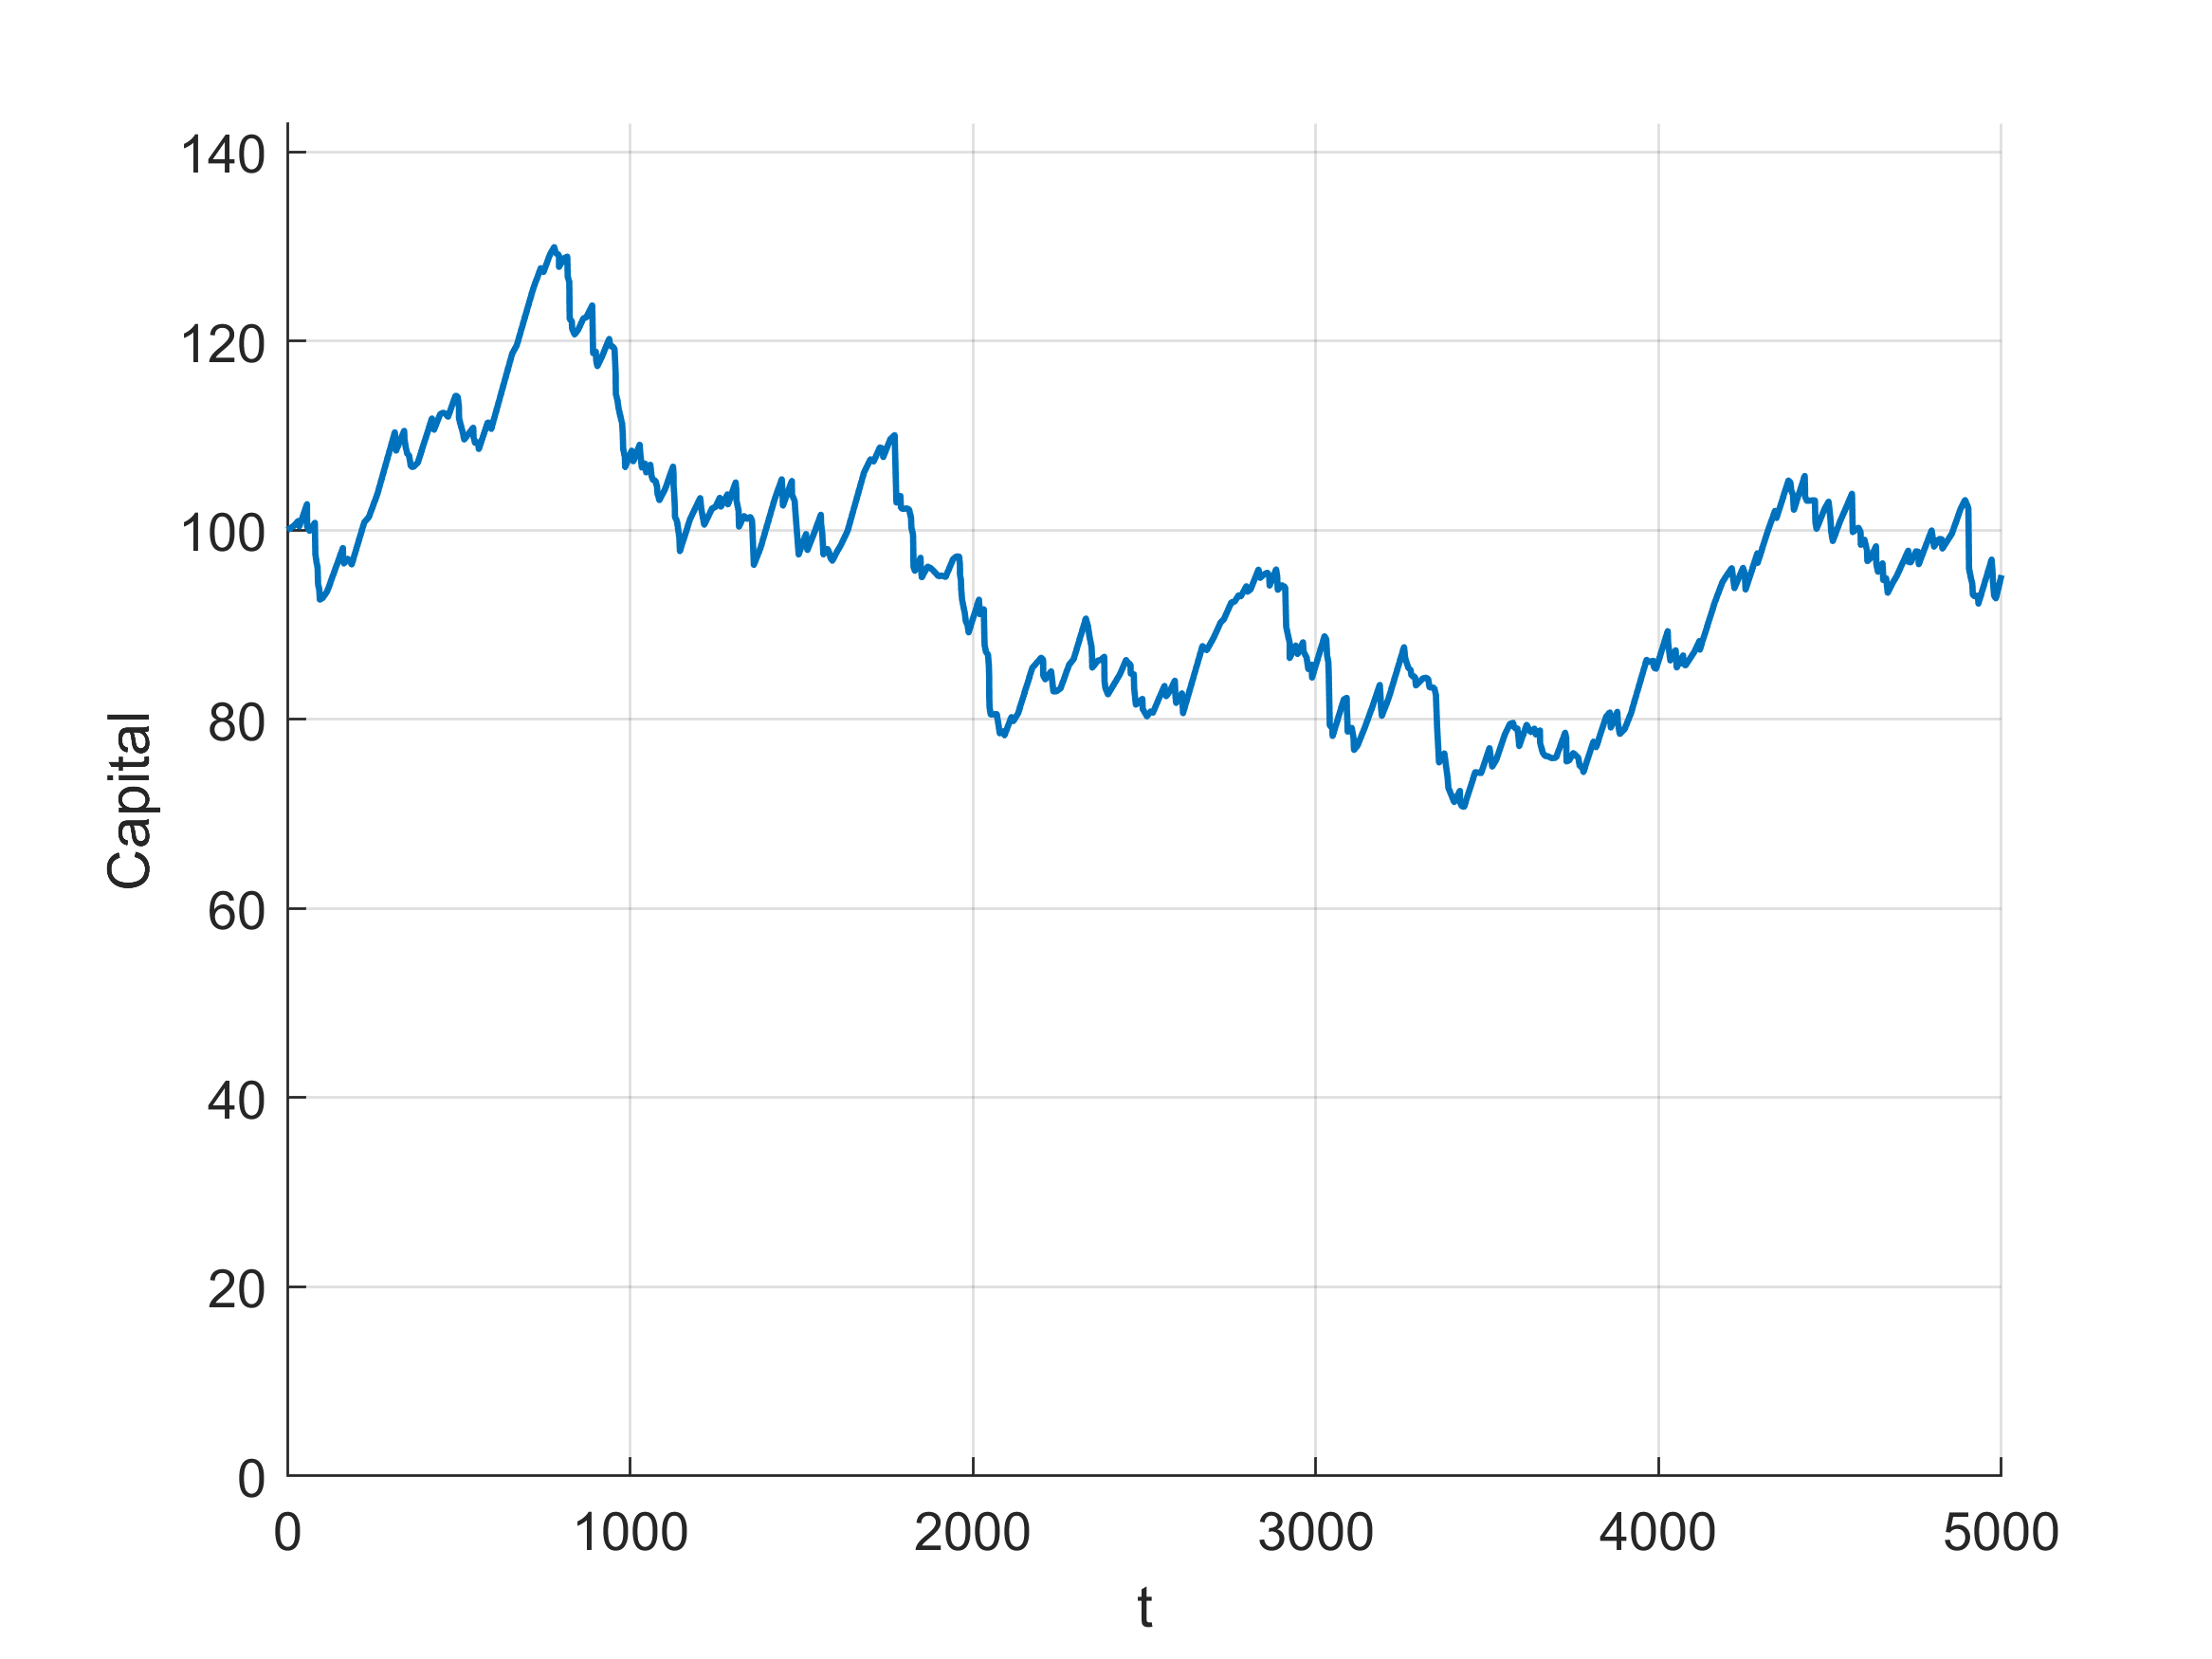
\includegraphics[width=0.6\textwidth]{../code/Task_11/pict/ins_10_100_15_3_ex.png}
				\caption{Капитал при $W_0 = 100, \lambda=  0.1, k=3, x_m =1, c =0.15, T=5000 $.}
		    \end{figure}
	\end{itemize}
\newpage
\section{Библиография}
	\begin{thebibliography}{99}
		\bibitem{smirnov} С.~Н.~Смирнов \textit{Лекции по стохастическому анализу}, 2019.
		\bibitem{th_ident} И.~В.~Востриков \textit{Лекции по теории идентификации}, 2019.
		\bibitem{feller} В.~Феллер \textit{Введение в теорию вероятностей и ее приложения}, 
			том 1. М: Мир, 1984.
		\bibitem{article} P.~A.~W.~Lewis \textit{Simulation of nonhomogeneous poisson proesses by thinning}, 1979.
	\end{thebibliography}


\end{document}












